%% Document %%
\documentclass[12pt, a4paper]{book}


%% Packages %%
\usepackage{breakcites}
\usepackage{ucs}
\usepackage{placeins} % donne \FloatBarrier pour forcer l'affichage de toutes les figures
\usepackage[utf8x]{inputenc}
\usepackage[francais]{babel}
\usepackage{graphicx}
\usepackage{mathpazo}  % Pour la police
\usepackage{fancyhdr}
\usepackage{multirow} % lignes soudées
\usepackage{hyperref}
\usepackage{amsmath}   % Pour numberwithin
\usepackage{fullpage}
\usepackage{pdfpages}
\usepackage[font={it}]{caption}

\usepackage{fix-cm}


%\setcounter{tocdepth}{2}
%%%%%%%%%%%%%%% Modification de la taille des captions
% \newcommand{\captionfonts}{\small\itshape}
% 
% \makeatletter  % Allow the use of @ in command names
% \long\def\@makecaption#1#2{%
%   \vskip\abovecaptionskip
%   \sbox\@tempboxa{{\captionfonts #1: #2}}%
%   \ifdim \wd\@tempboxa >\hsize
%     {\captionfonts #1: #2\par}
%   \else
%     \hbox to\hsize{\hfil\box\@tempboxa\hfil}%
%   \fi
%   \vskip\belowcaptionskip}
% \makeatother   % Cancel the effect of \makeatletter
%%%%%%%%%%%%%%% Find de la modification


%% Metadata %%
\title{Manuscrit de Thèse}
\author{Simon Marache-Francisco}
\date{\today}


%% Data %%
\begin{document}
\sloppy



% espace interr-paragraphe un peu plus grand
\addtolength{\parskip}{0.5em}


%\numberwithin{section}{part} 
%%%%%%% pour éloigner le texte de la tables des matières des nombres
%\renewcommand{\cftsecaftersnumb}{\hspace{1em}}
%\renewcommand{\cftsubsecaftersnumb}{\hspace{1em}}
%\renewcommand{\cftsubsubsecaftersnumb}{\hspace{1em}}

% ############################# Paramètres PERSO

\newcommand{\todo}[1]{
\addcontentsline{toc}{subsection}{\textbf{Todo:} #1}
$\|$\textbf{A Faire : }#1$\|$
}


\begin{titlepage}

\begin{center}

% Changements pour manuscrit final :
% Modification du fichier MLEM.pdf pour changer les H en R
% Ajout de la date sur la première page
% Choix de Christophe Odet comme président du Jury
% Rechercher une erreur dans la formule sur la projection/retro-projection (3.3 p. 40), i devient j ds somme (verifie publi OSEM)
% Changer les couleurs des lignes des courbes F-ROC pour qu'elles correspondent

% A faire vérifier :
% Mettre ensemble conclu & perspectives (conclu. trop petite)

% A Faire :
% Ajouter remerciements
% INDIQUER NUMERO D'ORDRE DANS LE FOLIO ADM + LA COUVERTURE A3

% Upper part of the page

\textbf{\Large Thèse}\\[0.5cm]

\textsl{\large Présentée devant}

\textsc{\large L’institut national des sciences appliquées de Lyon}\\[1.5cm]

\textsl{\large Pour obtenir}

\textsc{\large Le grade de docteur}\\[1.5cm]

\textsl{\large École doctorale: \'Electronique, \'Electrotechnique, Automatique}\\%[1.5cm]
\textsl{\large Formation doctorale : Images et Systèmes}\\[1cm]
\textsl{\large Par}

\textsc{\large Simon Marache-Francisco}\\\textsl{(Ingénieur INSA Rouen)}\\[1.5cm]

\textbf{\LARGE \'Evaluation de la correction du mouvement respiratoire sur la détection des lésions en oncologie TEP}\\[1.5cm]

\textsl{\large Soutenue le 14/02/2012 devant la Commission d’examen}\\[1cm]

\vfill 

\begin{flushleft} \textbf{\Large Jury :} \end{flushleft}
% Title

%\rule{\linewidth}{0.2 em}

\begin{tabular}{l l l}
Président	& Christophe Odet	&	Professeur, CREATIS, INSA-lyon\\
\\
Rapporteur 	& Michel Desvignes	&	Professeur, GIPSA-Lab, INP Grenoble\\
Rapporteur 	& Su Ruan		&	Professeur, LITIS, Université de Rouen\\
\\
Examinateur	& Frédéric Lamare	&	Docteur, Ingénieur de Recherche, INCIA\\
Examinateur	& Jean-Michel Rouet	&	Docteur, Ingénieur Philips Healthcare Medisys\\
\\
Co-encadrante	& Carole Lartizien	&	Chargée de Recherche CNRS, CREATIS, Lyon\\
Directeur de thèse& Rémy Prost		&	Professeur, CREATIS, INSA-Lyon\\




% 
% Rapporteur	& M. Desvignes & Professeur (Grenoble-INP)\\
% 	& F. Lamare	& Ingénieur de recherche (CHU Pellegrin Bordeaux) \\
% 	& C. Lartizien	& Chargé de Recherche\\
% 	& R. Prost	& Professeur (INSA Lyon)\\
% Rapporteur	& S. Ruan	& Professeur (Université de Rouen)\\
% 	& J.M. Rouet	& Ingénieur R.\&D. (Philips Medisys)\\
\end{tabular}



\end{center}

\end{titlepage}

~~~
\newpage

\pagestyle{fancyplain}
\setlength{\headheight}{17pt}
\setlength{\headsep}{35pt}
%\setlength{\topmargin}{15pt}
%\setlength{\voffset}{10pt}

\lhead{\fancyplain{}{}}
\chead{}
\rhead{\fancyplain{}{\textit{\leftmark}}}
\lfoot{}
\cfoot{}
\rfoot{\thepage}


\renewcommand{\headrulewidth}{0pt}
\renewcommand{\footrulewidth}{0pt}

\addcontentsline{toc}{part}{Résumé} %\resizebox{4cm}{!}{\Huge Résumé}
{\fontsize{30}{100}\selectfont Résumé}

\rule{15cm}{0.1em}

\vspace{1cm}

\thispagestyle{plain}

La tomographie par émission de positons (TEP) est une méthode d’imagerie clinique en forte expansion dans le domaine de l’oncologie. De nombreuses études cliniques montrent que la TEP permet, d’une part de diagnostiquer et caractériser les lésions cancéreuses à des stades plus précoces que l’imagerie anatomique conventionnelle, et d’autre part d’évaluer plus rapidement la réponse au traitement. Le raccourcissement du cycle comprenant le diagnostic, la thérapie, le suivi et la réorientation thérapeutiques contribue à augmenter le pronostic vital du patient et maîtriser les coûts de santé.

La durée d’un examen TEP, de l’ordre de 5 à 10 minutes pour un champ de vue axial de l’ordre de 15 cm, ne permet pas de réaliser une acquisition sous apnée. La qualité des images TEP est par conséquent affectée par les mouvements respiratoires du patient qui induisent un flou dans les images. Les effets du mouvement respiratoire sont particulièrement marqués au niveau du thorax et de l’abdomen.

Plusieurs types de méthode ont été proposés pour corriger les données de ce phénomène, mais elles demeurent lourdes à mettre en place en routine clinique. La problématique de la correction du mouvement respiratoire et le choix de la méthode appropriée sont des sujets d’actualité au sein de la communauté de médecine nucléaire. Des travaux récemment publiés proposent une évaluation de ces méthodes basée sur des critères de qualité tels que le rapport signal sur bruit ou le biais. Aucune étude à ce jour n’a évalué l’impact de ces corrections sur la qualité du diagnostic clinique. Ce problème pose des questions d’orientation stratégique et financière importantes.

Nous nous sommes focalisés sur la problématique de la détection des lésions du thorax et de l'abdomen de petit diamètre et faible contraste, qui sont les plus susceptibles de  bénéficier de la correction du mouvement respiratoire en routine clinique.

Nos travaux ont consisté dans un premier temps à construire une base d’images TEP qui modélisent un mouvement respiratoire non-uniforme, une variabilité interindividuelle et contiennent un échantillonnage de lésions de taille et de contraste variable. Ce cahier des charges nous a orientés vers les méthodes de simulation Monte Carlo qui permettent de contrôler l’ensemble des paramètres influençant la formation et la qualité de l’image. Une base de 15 modèles de patient a été créée en adaptant le modèle anthropomorphique XCAT sur des images tomodensitométriques (TDM) de patients. Cette base contient 280 lésions sphériques de 8 et 12 mm diamètre réparties dans les poumons et le foie et dont le contraste a été calibré pour échantillonner la gamme de détection. Le signal respiratoire simulé est constitué d’un motif de 4 cycles mesurés sur des patients. Nous avons ensuite développé un protocole de simulation à l’aide du logiciel PET-SORTEO afin de générer les examens virtuels de chacun des modèles en considérant deux types d’acquisition : une acquisition dynamique en mode-liste synchronisée sur le signal respiratoire et une acquisition statique de même durée que l’acquisition dynamique mais correspondant au cas idéal d’un patient qui pourrait retenir sa respiration.

Nous avons en parallèle développé une stratégie originale d’évaluation des performances de détection. Cette méthode comprend un système de détection des lésions automatisé basé sur l'utilisation de machines à vecteurs de support (SVM) utilisant des caractéristiques fréquentielles. Les performances sont mesurées par l’analyse psychophysique des courbes free-receiver operating characteristics (FROC) que nous avons adaptée aux spécificités de l’imagerie TEP. L’évaluation des performances a été est réalisée sur deux méthodes prometteuses de correction du mouvement respiratoire (faut-il en dire un peu plus ?), en les comparant avec les performances obtenues sur les images non corrigées ainsi que sur les images idéales sans mouvement respiratoire. 
Les résultats obtenus sont prometteurs et montrent une réelle amélioration de la détection des lésions après correction, qui approche les performances obtenues sur les images statiques. 

\textsc{Mots-Clefs :} TEP, oncologie, mouvement respiratoire, reconnaissance de formes, Computer Aided Detection, Séparateurs à vaste marge, Simulation

\newpage

\addcontentsline{toc}{part}{Table des matières} \tableofcontents


%%%% A PLACER QUELQUEPART
%Elle permet l'évaluation de l'état d'avancement de la maladie, ou encore d'étudier la réponse à un traitement~\cite{dimitrakopoulou2002role}. Cette détection se fait actuellement par le médecin qui va observer les images TEP/TDM acquises à la recherche de fixations anormales. Cependant, ces fixations peuvent provenir d'autres facteurs, tels que la ``graisse brune'', des muscles activés ou encore une inflammation locale~\cite{bordessoule2006impact}. Du fait des limites de l'imageur au niveau du rapport signal sur bruit des volumes reconstruits, il est possible qu'il y ait une erreur de diagnostic.


%\part{Introduction}
\newpage


\addcontentsline{toc}{part}{Liste des figures} \listoffigures

\addcontentsline{toc}{part}{Liste des tables} \listoftables

\newpage

\addcontentsline{toc}{part}{Introduction}
\resizebox{10cm}{!}{\Huge Introduction}

\rule{15cm}{0.1em}

\vspace{3cm}

La tomographie par émission de positons (TEP) couplée à un tomodensitomètre (TDM) est une méthode d’imagerie clinique en forte expansion dans le domaine de l’oncologie. De nombreuses études cliniques montrent que la TEP permet, d’une part de diagnostiquer et caractériser les lésions cancéreuses à des stades plus précoces que l’imagerie anatomique conventionnelle, et d’autre part d’évaluer plus rapidement la réponse au traitement. Le raccourcissement du cycle comprenant le diagnostic, la thérapie, le suivi et la réorientation thérapeutiques contribue à augmenter le pronostic vital du patient et maîtriser les coûts de santé.

L’examen TEP/TDM au FDG apparaît désormais indispensable pour évaluer la réponse thérapeutique des patients atteints de lymphome. Les résultats préliminaires sont également très encourageants dans les tumeurs solides, en particulier les cancers pulmonaires, digestifs et de la sphère ORL~\cite{cachin2006evaluation}. La TEP pourrait prédire très précocement la réponse et ainsi permettre une réadaptation du schéma thérapeutique. Enfin de nouveaux traceurs TEP ouvrent la voie de l’imagerie moléculaire qui semble extrêmement prometteuse en thérapie génique et dans le suivi du traitement ciblé du cancer.

La durée d’un examen TEP, de l’ordre de 5 à 10 minutes pour un champ de vue axial de l’ordre de 15 cm, ne permet pas de réaliser une acquisition sous apnée. La qualité des images TEP est par conséquent affectée par les mouvements respiratoires du patient qui induisent un flou dans les images. Les effets du mouvement respiratoire sont particulièrement marqués au niveau du thorax et de l’abdomen. Deux types de méthode ont été proposés pour corriger les données de ce phénomène. Le premier type est basé sur l’utilisation d’acquisitions synchronisées sur la respiration produisant plusieurs images non affectées par la respiration et correspondant à différents instants du cycle respiratoire~\cite{nehmeh2002effect}\cite{boucher2004respiratory}. Cette méthodologie se base sur l’hypothèse  d’une grande régularité du signal respiratoire de synchronisation~\cite{boucher2004respiratory}, et conduit à des images d’une qualité statistique limitée car chacune ne contient qu'une fraction réduite du nombre de photons détectés pendant toute l’acquisition~\cite{visvikis2004evaluation}. Le deuxième type de méthode se base sur l’utilisation d’un scanner 4D TEP/TDM du patient permettant de modéliser les mouvements respiratoires. Ce modèle est alors intégré lors du processus de reconstruction tomographique~\cite{lamare2007list}. Ce type de méthode permet de pouvoir conserver la statistique de l’image mais nécessite une information anatomique dynamique assez lourde à acquérir en routine clinique.

La problématique de la correction du mouvement respiratoire et le choix de la méthode appropriée sont des sujets d’actualité au sein de la communauté de médecine nucléaire. Des travaux récemment publiés proposent une évaluation de ces méthodes basée sur des critères de qualité tels que le rapport signal sur bruit ou le biais~\cite{visvikis2004evaluation}. Aucune étude à ce jour n’a évalué l’impact de ces corrections sur la qualité du diagnostic clinique. Ce problème pose des questions d’orientation stratégique et financière importantes, puisque le second type de méthode requiert l’acquisition de données TEP/TDM dynamiques, très peu accessibles à l’heure actuelle.

C'est dans l'optique de résoudre ce problème que j'ai commencé ma thèse sur l'\textbf{Estimation des apports de la correction du mouvement respiratoire en oncologie TEP}.



La première partie de ca manuscrit va présenter l'imagerie TEP. Nous détaillerons les principes physiques de la TEP, le déroulement des acquisitions ainsi que les algorithmes de reconstruction utilisés pour former les images.

Ensuite, nous présenterons un état de l'art sur le mouvement respiratoire et sa correction dans les images TEP.

La troisième partie portera sur l'évaluation des performances de détections et sur les systèmes de détection utilisés pour mesurer ces performances.

Enfin, nous présenterons nos travaux : en premier lieu nous présenterons la base de données que nous avons créée pour réaliser les mesures de performances, puis la méthode utilisée pour répondre à la problématique, et enfin les résultats que nous avons obtenus.

La dernière partie corresponds aux discussions et perspectives sur notre travail.

\part{Imagerie TEP}
	\pagestyle{fancyplain}

\label{lab:chapPET}
La Tomographie par \'Emission de Positons (TEP) au fluorodesoxyglucose marqué au Fluor 18 ($^{18}$FDG) est une modalité d'imagerie fonctionnelle utilisant la désintégration d'un traceur radioactif pour mettre en valeur les zones de forte activité métabolique. Elle est principalement utilisée en imagerie cérébrale, oncologique et cardiologique.


Dans ces trois chapitres, nous allons tout d'abord détailler rapidement les principes physiques amenant à la création des images TEP, de la désintégration du traceur radioactif à la détection des photons émis lorsqu'ils atteignent un capteur. Ensuite, nous parlerons des solutions techniques mises en place pour réaliser les images TEP, avec les différents types d'acquisitions. Enfin, nous détaillerons les algorithmes utilisés pour reconstruire les images TEP.

 
\chapter{Principe Physique}

	\section{Généralités}

L'imagerie TEP est basée sur l'injection d'une molécule traceuse marquée par un atome radioactif émetteur de positon. Ce paragraphe présente rapidement les événements qui se produisent lors d'un examen TEP, présentés dans la figure~\ref{fig:schemaTEP}.

Ce traceur est conçu de manière à se fixer sur les zones du corps que l'on souhaite imager. Pendant toute la durée de l'examen, les particules radioactives vont se désintégrer selon la loi de décroissance radioactive de l'équation~\ref{eq:loidecradioact}.

\begin{equation}
	dN = - \lambda N dt
	\label{eq:loidecradioact}
\end{equation}

$N$ représente le nombre de particules radioactives présentes dans le corps du patient. $dN$ représente la variation de ce nombre de particules (le nombre de désintégrations par $dt$) et $\lambda$ est une constante dépendant de l'élément radioactif.

Chaque désintégration d'un élément radioactif va déclencher l'émission d'une particule chargée $\beta^+$, aussi appelée positon. En oncologie, on utilise par exemple le Fluor $^{18}F$ qui se désintègre en Oxygène $^{18}O$ en émettant un positon. Cette particule va parcourir quelques mm avant de s'annihiler avec un électron en émettant 2 photons dans deux directions opposées avec une énergie de 511 KeV.

Ce sont ces photons qui sont détectés par l'imageur TEP. Ils représentent une coïncidence, car l'instant d'arrivée et leur énergie sont semblables. L'ensemble des ``Lignes de réponse'' (LDR) correspondant aux coïncidences détectées est utilisé pour reconstruire les images.

\begin{figure}
\centering
\includegraphics[width=16cm]{images/schemaTEP}
\caption[Présentation simplifiée de la TEP]{Processus d'un examen TEP : a) Injection du traceur radioactif, qui va se fixer préférentiellement sur les zones que l'on cherche à observer. b) Désintégration d'un atome radioactif du traceur, ici dans la zone à imager. Cela entraîne l'émission de deux photons dans deux directions opposées, qui sont détectés dans la couronne de capteurs. c) Tous les événements détectés sont stockés dans la mémoire de la console, ici sous forme de sinogramme. d) L'image est reconstruite à la suite de l'acquisition pour former un volume 3D estimant la répartition du traceur dans l'organisme.}
\label{fig:schemaTEP}
\end{figure}


\section{Traceur $^{18}$FDG}

Le glucose est considéré comme un carburant essentiel à l’organisme qui peut l’assimiler directement. Les cellules cancéreuses, qui ont un métabolisme accéléré par rapport aux autres cellules du milieu, sont particulièrement friandes de glucose. Celui-ci est transporté à l’intérieur des cellules par des transporteurs spécifiques de la membrane afin d’être dégradé par un ensemble de réactions appelé glycolyse. Le glucose est d’abord phosphorylé en glucose-6-phosphate, catalysé par l’enzyme hexokinase. Le glucose-6-phosphate est ensuite transformé en fructose-6-phosphate qui subit à son tour plusieurs transformations successives pour être finalement excrété par la cellule sous forme de lactate.

Le fluorodeoxyglucose ou FDG est un analogue du glucose avec un aspect structural très proche. Il est donc aussi capté par les cellules, mais ne peut pas être utilisé dans leur métabolisme. Le FDG suit le même processus métabolique que le glucose jusqu’à l’étape de phosphorylation en FDG-6-phosphate. Il n’est cependant pas métabolisé par l’enzyme glucose-6-phosphate et s’accumule dans la cellule sous la forme de FDG-6-phosphate. Cette accumulation permet de distinguer la présence de tumeurs, généralement beaucoup plus gourmandes en énergie que les tissus sains et donc marquées par une présence élevée de FDG-6-phosphate. Par son métabolisme et son importance pour les cellules cancéreuses, le FDG est actuellement préconisé en clinique pour les examens concernant des patients en cancérologie. Il est généralement marqué au fluor 18 donnant le $^{18}$FDG.

Cependant, ce radiotraceur n'est pas spécifique aux tumeurs mais se fixe sur toute cellule consommant du glucose. C'est pourquoi le coeur ainsi que le cerveau fixent toujours une grande quantité de $^{18}FDG$, comme l'indique la figure~\ref{fig:schemaTEP}.

\section{\'Emission des photons}

Nous allons maintenant détailler le processus qui déclenche l'émission des photons détectés par l'imageur, présenté dans la figure~\ref{fig:Langner2008ad}.

Les émetteurs de positons utilisés en TEP sont des isotopes radioactifs présentant un excès de charge positive, ou proton, dans leurs noyaux. Un processus de désintégration $\beta^+$, correspondant à la transformation d’un proton $p$ en un neutron $n$, leur permet de migrer vers un état stable. Cette désintégration résulte en l’émission d’un neutrino $\nu$ et d’un positon $e^+$ selon l’équation~\ref{eq:desinteg}. Le positon est une particule de même masse que l’électron mais de charge opposée.

\begin{equation}
 p~\rightarrow~n + e^+ + \nu
\label{eq:desinteg}
\end{equation}

Le positon va alors s'annihiler avec un électron après un parcours de quelques millimètres en émettant simultanément deux photons $\gamma$ de même énergie (511 keV), comme indiqué dans l'équation~\ref{eq:annihilation}. L'angle d'émission des photons $\gamma$ est de $180°$ avec une incertitude de $\pm 0.25°$~\cite{bailey2005positon}.

\begin{equation}
 e^+ + e^-~\rightarrow~\gamma + \gamma
\label{eq:annihilation}
\end{equation}

\begin{figure}
\centering
\includegraphics[width=12cm]{images/annihilation}
\caption[\'Emission des photons]{\'Emission des photons~\cite{Langner2008ad} : Le radio traceur se désintègre en émettant un neutrino et un positon. Après un parcours de quelques mm dans les tissus, ce dernier s'annihile avec un électron. Cette réaction provoque la création de deux photons $\gamma$ d'énergie 511 keV partant dans deux directions opposées.}
\label{fig:Langner2008ad}
\end{figure}

\section{Détection des photons}

Les détecteurs les plus couramment utilisés en TEP sont constitués d'un couplage entre un cristal scintillant et un tube photomultiplicateur.

Le cristal scintillant permet de convertir les photons $\gamma$ de 511 keV en photons lumineux par les différents phénomènes d'interaction particules-matières.

Chaque photon absorbé par le matériau scintillant va entraîner une réaction en chaîne qui va déclencher une émission lumineuse. Le tube multiplicateur situé derrière va convertir cette émission lumineuse en charge électrique. Un système électronique va ensuite apparier les photons détectés pour retrouver la ligne de réponse (LDR) sur laquelle la désintégration a eu lieu. Les paires de photons assemblées correspondent à des coïncidences.

Les détecteurs sont regroupés par modules, placés en anneaux autour du patient. L'imageur TEP Gemini que nous utiliserons dans cette étude dispose par exemple de 28 modules, contenant chacun une matrice de 29 par 22 cristaux de GSO~\ref{fig:moduleTEP}. Une photo de l'imageur ouvert est visible sur la figure~\ref{fig:gemini_ecl}. 420 Photomultiplicateurs placés autour des blocs sont utilisés pour estimer la position des détections.

\begin{figure}
\centering
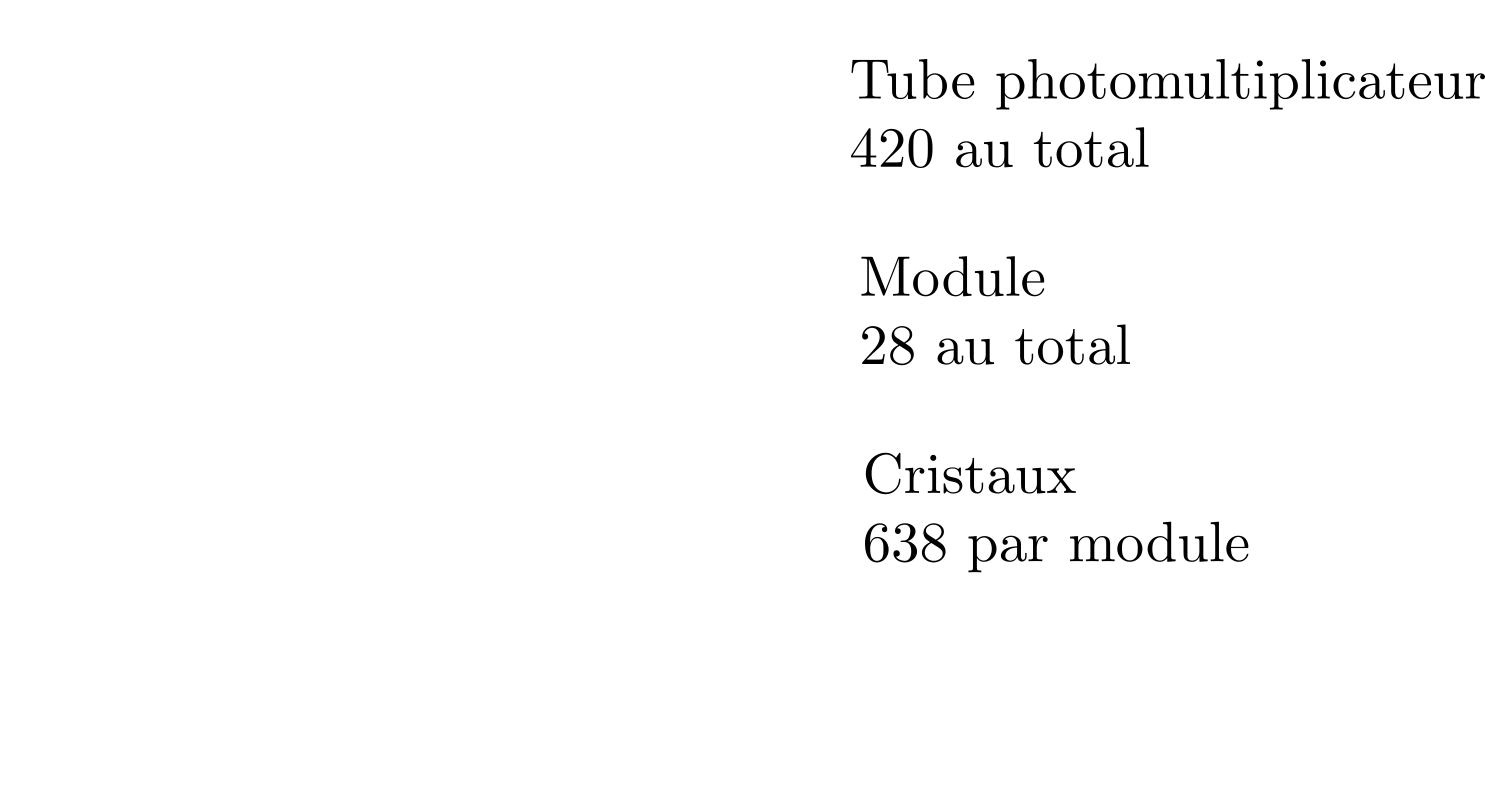
\includegraphics[width=8cm]{images/coupe_module}
\caption[Coupe d'un module de Philips Allegro]{Coupe d'un module de Philips Allegro. Les 28 modules sont placés en anneaux autour du patient.}
\label{fig:moduleTEP}
\end{figure}


\begin{figure}
\centering
\includegraphics[width=12cm]{images/gemini_eclate}
\caption[Photo d'un imageur Philips Gemini ouvert]{Cette photo représente la partie PET d'un imageur Philips Gemini ouverte. On distingue les cartes électroniques connectées aux tubes photomultiplicateurs.}
\label{fig:gemini_ecl}
\end{figure}

	\section{Types de coïncidences}

La figure~\ref{fig:schemaDetections} représente les différents types de coïncidences rencontrés en TEP.

Les coïncidences vraies (\ref{fig:schemaDetections}.a) correspondent aux cas où les deux détections appariées correspondent bien à une seule désintégration et où aucun des photons n'a été dévié. Les coïncidences fortuites (\ref{fig:schemaDetections}.b) correspondent à la détection en coïncidence de deux photons issus de deux annihilations différentes, par exemple à cause de l’absorption d’un des photons d’une désintégration par les tissus. Enfin, les coïncidences diffusées (\ref{fig:schemaDetections}.c) sont le résultat de la déviation d'un des deux photons produit engendré par des interactions rayonnement-matière dans les tissus (diffusion Compton). 

%Pour éliminer ces erreurs, un certain nombre de méthodes ont été implémentées, dont le filtrage en énergie et en temps au niveau matériel : ne sont prises en compte que les paires d'événements arrivant dans une fenêtre temporelle et énergétique définie. En effet, les photons déviés vont perdre de l'énergie, ce qui va entraîner leur élimination.

%\todo{pkoi barré?}

Les coïncidences diffusées ainsi que les coïncidences aléatoires génèrent un bruit parasite dans les sinogrammes. L'absorption des photons sans détection va engendrer un effet d'atténuation du signal qui sera de plus en plus important en fonction de la profondeur des tissus et de leur absorption.


\begin{figure}
\centering
\includegraphics[width=12cm]{images/schemaDetections}
\caption[Les différents types de coïncidences en TEP]{Les différents types de coïncidences en TEP. Le trajet réel du photon est indiqué en trait fin simple, tandis que la ligne de réponse est indiquée en trait pointillé épais. On appelle les coïncidences vraies (a) lorsque l'annihilation est bien sur la ligne de réponse, fortuites (b) lorsque deux désintégrations réalisées en même temps sont considérées comme une seule et diffusée (c) lorsqu'un des photons est dévié.}
\label{fig:schemaDetections}
\end{figure}



	\section{Perturbation du trajet du photon}

Les deux interactions les plus importantes que peuvent avoir les photons avec les tissus sont la diffusion Compton et l'absorption photo-électrique~\cite{cherry2006pet}. L'effet Rayleigh, qui correspond à la diffusion du photon sur un atome, est peu présent aux énergies concernées par la TEP. 

La diffusion Compton correspond à l'interaction entre le photon émis et un électron du milieu. L'énergie cinétique de l'électron est augmentée, tandis que le photon est dévié. Il est intéressant de noter qu'une déviation de 25° engendre une perte d'énergie du photon de seulement 10\%~\cite{evans1955atomic}.

L'absorption photo-électrique correspond quant à elle à l'interaction entre un noyau atomique et un des photons. L'énergie du photon est absorbée par le noyau et transmis à un de ses électrons. 

L'atténuation du signal est liée à une combinaison de ces effets. L'effet d'atténuation est particulièrement important en TEP, car il génère des artefacts très visibles, qui doivent être corrigés à partir d'une carte d'atténuation, déduite d'un examen de tomodensitométrie (tomographie par rayons X) ou d'une carte de transmission, comme indiqué sur la figure~\ref{fig:schemaAtt}.


On peut représenter cette atténuation de manière analytique à l'aide de la loi de Beer-Lambert~\cite{cherry2006pet}, qui montre que l'atténuation augmente exponentiellement avec la longueur du trajet dans les tissus :
\begin{equation}
I = I_0 e^{-\mu l}
\end{equation}

Avec $I_0$ la quantité originale de photons, $I$ le nombre de photons qui traversent le milieu, $\mu$ le coefficient d'atténuation du milieu et $l$ la longueur du trajet. 

Dans le cas où le milieu est complexe, et si l'on connaît l'atténuation $\mu(x)$ en chaque point $x$ du trajet, on peut connaître précisément l'atténuation subie selon chaque ligne de réponse  :

\begin{equation}
I = I_0 e^{- \int\limits^L_0 \mu(l) dl}
\end{equation}


\begin{figure}
\centering
\includegraphics[width=12cm]{images/attenuationNonAtt}
\caption[Effet de l'atténuation sur les images TEP]{Effets de l'atténuation sur des images TEP : L'image de gauche correspond à la distribution de radioactivité reçue par les détecteurs. On peut observer une perte progressive de l'activité vers l'intérieur des tissus, car les photons ont plus de chances d'interagir avec la matière. L'image TDM au centre est utilisée pour estimer une carte de l'atténuation des tissus et prendre en compte cette atténuation lors de la reconstruction de l'image TEP.}
\label{fig:schemaAtt}
\end{figure}

\section{Quantification en imagerie TEP}

L'image visualisée par le clinicien est directement liée à  la concentration de l'isotope radioactif. La concentration observée est la somme de la concentration du traceur piégé dans les cellules et du traceur libre dans le compartiment vasculaire. Cette concentration mesurée est très dépendante du volume du patient, ainsi que de la dose injectée.

En clinique, on utilise habituellement le SUV (Standard Uptake Value), qui est un index semi-quantitatif permettant de s'affranchir de la dose injectée et des caractéristiques morphologiques du patient. Cela permet de réaliser des comparaisons entre des fixations radioactives de plusieurs examens, voire de plusieurs patients.

Le SUV est défini comme suit :

\begin{equation}
SUV=\frac{C}{ \frac{dose~inject\acute{e}e}{poids~corporel} }
\end{equation}

Où C est la concentration du traceur radioactif.

Des méthodes, plus complexes, basées sur des acquisitions dynamiques et la connaissance \textit{a priori} d'un modèle de distribution du traceur dans l'organisme, permettent de remonter à des paramètres biologiques, tels que la consommation de glucose par gramme de tissus et par unité de temps pour le FDG. Ces méthodes sont en pratique peu utilisées en routine clinique en raison de la difficulté et du coût de réalisation des acquisitions dynamiques.

\chapter{Déroulement d'une acquisition}


Nous allons maintenant décrire rapidement quelques points techniques permettant de mieux comprendre comment sont réalisées les acquisitions TEP en routine clinique. Nous parlerons de la méthode utilisée pour réaliser des acquisitions corps entier alors que l'imageur a un champ de vue axial limité et des contraintes associées. Enfin, nous aborderons la problématique du format des données et ses implications.

\section{TEP au $^{18}$FDG}


En oncologie, les patients qui ont une suspicion de cancer se voient proposer un examen TEP pour réaliser un diagnostic initial, qui va viser à déterminer le degré de malignité de la pathologie détectée. Il a été montré~\cite{gould2001accuracy} que les performances de la TEP sur la détection des lésions pulmonaires étaient supérieures à l'imagerie anatomique. Les performances de la TEP sont aussi reconnues pour les cancers hépatiques et la détection précoce des lymphomes. Plusieurs images sont visibles dans la figure~\ref{fig:exTEP}.

La TEP est ensuite utilisée pour suivre l'évolution des lésions, afin d'adapter le traitement à l'évolution de la maladie.

\begin{figure}[h!]
\centering
\begin{tabular}{c c c}
\includegraphics[width=5cm]{images/ex_lymphome} & \includegraphics[width=5cm]{images/ex_poumon} & \includegraphics[width=5cm]{images/ex_cou} \\
a) & b) & c)
\end{tabular}
\caption[Exemples d'images TEP]{Exemples d’images TEP au $^{18}$FDG provenant d’examens de patients atteints d’un cancer a) des ganglions (lymphome), b) du poumon et c) du cou. Certaines lésions sont représentées par les flèches noires.}
\label{fig:exTEP}
\end{figure}

\section{Acquisitions corps entier}


Les acquisitions TEP réalisées pour l'oncologie sont habituellement des acquisitions corps entier, de manière à pouvoir avoir une vue de l'étendue des lésions.

Or le champ de vue axial de la plupart des caméras TEP est de l'ordre de 15 à 20 cm environ (18 cm pour le Philips allegro~\cite{lamare2006validation}). En routine clinique, le patient est placé sur un lit qui se déplace par incréments successifs lors de l'acquisition. Une photographie de l'imageur avec le lit est présentée dans la figure~\ref{fig:photoGemini}.

\begin{figure}
\centering
\includegraphics[width=12cm]{images/gemini}
\caption[Photographie d'un scanner TEP gemini]{Photographie d'un scanner TEP/TDM Gemini. Le lit motorisé est présenté au premier plan et permet de faciliter le déplacement du patient au cours de l'acquisition.}
\label{fig:photoGemini}
\end{figure}

Le nombre de positions du lit est déterminé par la taille du patient ainsi que par le champ de vue du tomographe. Chaque lit est reconstruit séparément puis assemblé avec les lits suivants et précédents, comme indiqué dans la figure~\ref{fig:multilits}. \'Etant donné que les caméras TEP ont une sensibilité plus faible à leurs extrémités, on introduit un chevauchement plus ou moins important dans les lits.

\begin{figure}
\centering
\includegraphics[width=10cm]{images/multilits}
\caption[Acquisitions corps entier en TEP]{Réalisation d'une acquisition corps entier en TEP : Chaque lit est acquis et reconstruit séparément avec un chevauchement. Les lits sont ensuite assemblés pour produire l'image finale.}
\label{fig:multilits}
\end{figure}

Les acquisitions corps entier utilisent typiquement plus de 10 lits sur la caméra Philips Gemini, ce qui demande un temps considérable. Il faut donc faire des compromis entre le temps d'acquisition et la qualité des images. Sachant que les examens TEP sont coûteux et que l'immobilité est inconfortable pour les patients, le temps d'acquisition est calibré pour durer moins d'une heure au total. Les nouvelles générations d'imageurs permettent cependant de réduire les temps d'acquisition à 2 minutes par lit à qualité équivalente.


	\section{Acquisition en mode 3D}

Historiquement, les données étaient acquises par coupe : des septas (plaque destinées à absorber les photons) étaient placés entre les détecteurs dans la dimension axiale de manière à éliminer les photons qui n'étaient pas émis dans le plan  transverse (perpendiculaire à l'axe du détecteur). Aujourd'hui, la totalité des scanners fonctionnent en mode 3D uniquement. Le retrait des septa (voir la figure~\ref{fig:2D3D}) permet d'augmenter le rapport signal sur bruit pour les gammes d'activité injectées aux patients, même si la détection des coïncidences vraies s'accompagne d'une augmentation de bruit parasite liée à l'augmentation de la détection des coïncidences fortuites et diffusées.

\begin{figure}
\centering
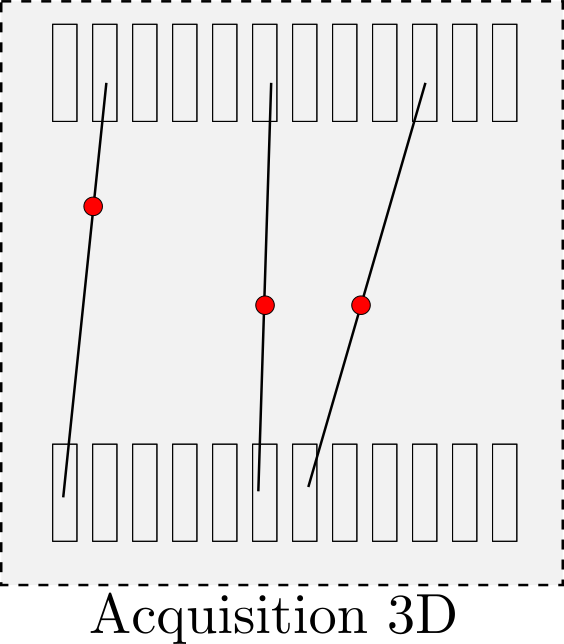
\includegraphics[width=6cm]{images/2D3D}
\caption[Acquisitions 3D en TEP]{Coupe schématique axiale d'un imageur TEP. Les annihilations représentées en rouge émettent des photons qui sont détectés par des cristaux correspondant à des plans de coupes différents}
\label{fig:2D3D}
\end{figure}


%	\section{Corrections}

	\section{Correction de l'atténuation}
\label{CorrectionAttenuation}

Le patient passe tout d'abord un examen TDM sur les scanners couplés TEP/TDM. Les valeurs des coefficients Hounsfield correspondant à l'atténuation des rayons X sont transformées pour correspondre à l'atténuation des photons de 511keV de la TEP. Cette image est ensuite utilisée pour réaliser la correction d'atténuation. 

Une technique plus ancienne d'estimation de la carte d'atténuation est basée sur une image acquise en transmission, où une source radioactive émettrice de positons est placée dans l'imageur et tourne autour du patient. Une acquisition  préalable est réalisée ``à blanc'', sans le patient. Le rapport entre la quantité de photons reçue par les détecteurs avec et sans le patient permet de générer la carte d'atténuation du corps du patient, de la même manière que pour l'imagerie TDM. Cependant, la généralisation des scanners couplés TEP/TDM limite l'utilisation de cette technique.

\begin{equation}
I(x) = I_0(x) e^{-\mu x}
\end{equation}

En connaissant la radioactivité reçue sans le patient (``à blanc'') $I_0$, la radioactivité reçue avec le patient $I$, on peut en déduire la valeur de $\mu$.

%\subsection{Correction des coïncidences fortuites}

%Des techniques existent pour corriger les données des effets vus dans la figure~\ref{fig:schemaDetections}, notamment l'implantation d'une ligne à retard pour estimer les coïncidences aléatoires puis les retirer du sinogramme.

	\section{Correction des autres sources de bruit}

\subsubsection{Correction de temps mort}


Le temps mort correspond à l’intervalle de temps durant lequel le dispositif est insensible après le passage d’une impulsion électrique. Lorsque deux impulsions surviennent avec un décalage temporel inférieur au temps d’intégration, seule la première est traitée et la deuxième est perdue. La correction de ce temps mort consiste à modéliser les pertes de comptage en événements pour chaque module de détection. En effet, le taux de photons simples $s$ et le facteur de temps mort, noté $d_{tk}$, sont liés par la relation \ref{eq:tm} où les constantes A et B apparaissant sont déterminées expérimentalement.

\begin{equation}
d_{tk} = 1 + As + Bs^2
\label{eq:tm}
\end{equation}



\subsubsection{Correction de coïncidences diffusées}

Les coïncidences diffusées, bien que déjà triées par les fenêtres énergétiques, peuvent excéder 50\% des coïncidences détectées. Les images non corrigées présentent une diminution du contraste, du rapport signal sur bruit et une perte en résolution spatiale. Trois types de méthodes existent afin de corriger les données de ces coïncidences diffusées : 
\begin{itemize}
\item Combinaison des données acquises dans au moins deux fenêtres en énergie.
\item Exploitation de l’information spatiale de localisation erronée des coïncidences diffusées.
\item Calcul direct de la distribution des coïncidences diffusées de manière analytique pour un patient donné, ou en utilisant des méthodes de simulation de type Monte Carlo.
\end{itemize}


\subsubsection{Correction des coïncidences aléatoires}
Les coïncidences aléatoires provenant de la détection de deux photons issus de deux annihilations différentes mais détectées dans la même fenêtre temporelle bruite les données mesurées. La correction de ce phénomène consiste à soustraire au niveau du sinogramme les coïncidences aléatoires estimées des coïncidences vraies. Ces coïncidences aléatoires peuvent être estimées de trois façons~\cite{brasse2005correction} :

\begin{itemize}
\item Utilisation d'une fenêtre temporelle décalée. L’activité y est considérée comme constante par sa taille réduite, mais les événements détectés proviennent forcément d’annihilations différentes par sa taille suffisamment élevée.
\item Estimation du taux de coïncidences aléatoires en connaissant le nombre total de photons détectés par chaque module : la distribution des coïncidences aléatoires est plus ou moins uniforme dans le champ de vue. Le taux d’événements aléatoires mesuré sur une LDR est fonction de la largeur de la fenêtre de coïncidences temporelles ($2\tau$) et des taux de photons simples (aussi appelé singles) détectés par les deux modules considérés.
\item Estimation à partir de la distribution des coïncidences dans les projections en dehors du patient.
\end{itemize}


\subsubsection{La normalisation}

Des différences de sensibilité de détection d’une source uniforme existent d’une LDR à l’autre, d’une part à cause de la forme des systèmes de détections, en général à anneaux circulaires; d’autre part à cause des différences d’incidence des photons par rapport à la face d’entrée du cristal et de l’efficacité individuelle du système de détection. Les méthodes de correction peuvent être basées sur l’inversion directe des données acquises à partir d’une source irradiant uniformément toutes les lignes de réponse. Elles peuvent aussi être basées sur des mesures traitées par un modèle mathématique reliant le facteur de normalisation pour une LDR entre deux cristaux à l’efficacité intrinsèque des détecteurs et une fonction de la sensibilité dépendant de l’arrangement géométrique des détecteurs.



	\section{Format des données}
Les données acquises par une caméra TEP peuvent être stockées sous deux formes principales : séquentielles et sinogramme.

		\subsection{Séquentielles}
\label{lab:modeliste}
Ce format correspond à un enregistrement ``brut'' des données issues de l'électronique de la caméra. Il est aussi appelé mode liste.

Ce format de fichier est en fait un enregistrement séquentiel des événements, dans leur ordre de détection. On peut enregistrer chaque photon détecté indépendamment, ou encore uniquement les coïncidences. Chaque événement est daté, ce qui permet de conserver l’information temporelle. On peut l'utiliser notamment pour synchroniser les données acquises avec le temps, pour la correction de mouvement par exemple, ou pour observer comment se répartit le radio-traceur au cours du temps.

Il existe plusieurs formats publiques de fichiers pour le stockage de ces données, notamment le format LMF (List-Mode Format) développé pour le projet ClearPET et le format ROOT développé par le CERN. Cependant, chaque constructeur utilise son propre format de fichier propriétaire.


Ce mode de stockage consomme une très grande quantité de ressources, étant donné qu'un examen PET est constitué de plusieurs millions d'événements. Cela engendre de fortes contraintes en espace disque et complique de beaucoup la manipulation des données. 

		\subsection{Sinogramme}

Le sinogramme est une matrice indiquant pour chaque ligne de réponse le nombre de détections réalisées, comme présenté dans la figure~\ref{fig:sino}. En ordonnés sont représentés les angles de la ligne de réponse, et en abscisse leur distance au centre du détecteur~\cite{fahey2002data}. Dans le mode 3D, on détecte des paires de photon qui ne sont pas directement dans le plan du détecteur. Une dimension supplémentaire correspondant à l'angle d'inclinaison de plans par rapport à l'axe du scanner est donc ajoutée pour prendre en compte cet effet.

Le principal avantage du sinogramme est qu'il permet de stocker les données acquises lors d'un examen TEP de manière beaucoup plus compacte que le format séquentiel. Cependant, il ne conserve aucune information temporelle ni énergétique.

\begin{figure}
\centering
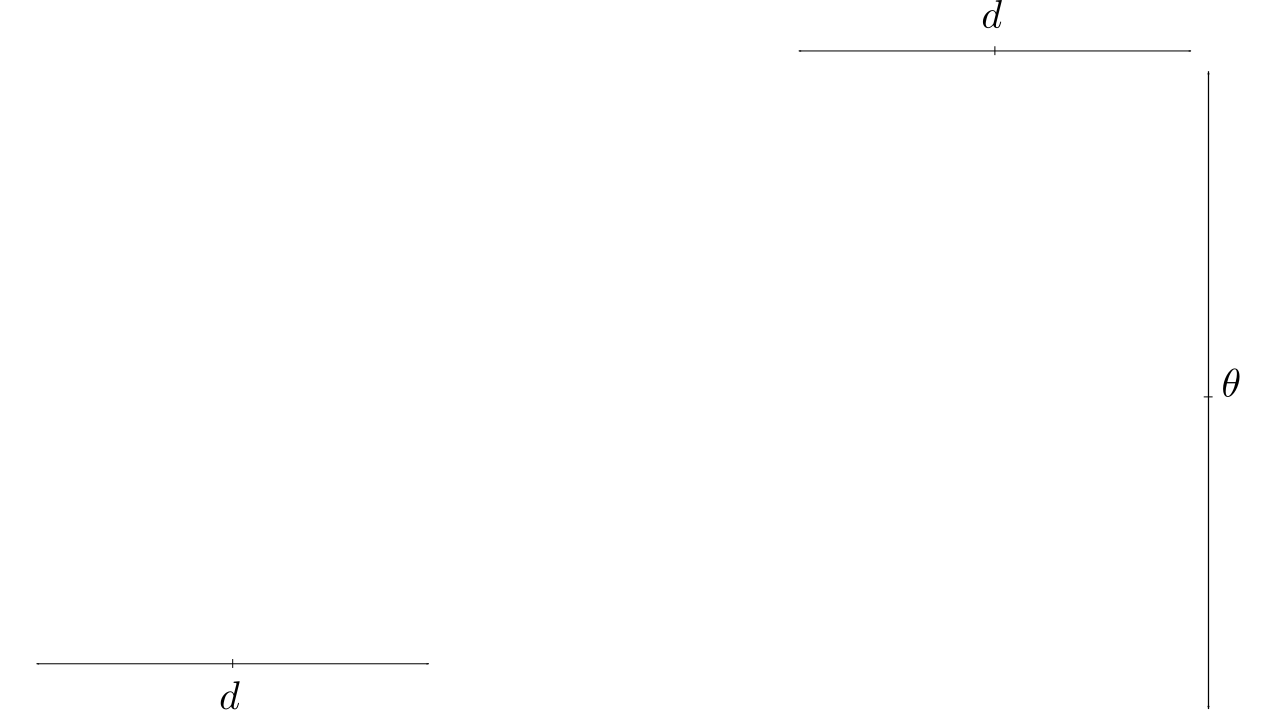
\includegraphics[width=11cm]{images/sino}
\caption[Principe du sinogramme]{Exemple de sinogramme: chaque ligne correspond à une projection de l'image selon un angle $\theta$ correspondant à la position de la ligne dans le sinogramme.}
\label{fig:sino}
\end{figure}











\chapter{Algorithmes de reconstruction}

La reconstruction des images TEP correspond à un problème inverse : à partir de l'ensemble des lignes de réponse, il faut déduire la répartition du radio traceur dans l'organisme du patient. Deux classes d'algorithmes existent pour résoudre ce type de problèmes, mais actuellement seuls les algorithmes itératifs sont utilisés en oncologie clinique. 

	\section{Algorithmes Itératifs}

La relation liant l'image TEP $f$ et les projections sur les détecteurs $p$ est la suivante :

\begin{equation}
	p = R f + e
\label{eq:eqTEP}
\end{equation}

Avec $R$ la matrice de projection et $e$ correspondant aux phénomènes parasites. Ce problème est mal posé, car la perte d'information due aux projections ne garantit pas la résolution de ce problème. De plus, le bruit est un élément perturbateur supplémentaire. Il nécessite donc l'utilisation d'algorithmes spécialisés. 


		\subsection{Algorithme ML-EM (Maximum Likelihood Expectation Maximisation) }


L'algorithme ML-EM~\cite{shepp1982maximum} est initialisé avec une image de départ $f_0$, et considère que les comptages des lignes de réponses $p_i$ sont indépendants et bruités selon une loi de Poisson. Il se déroule en deux phases principales : une phase de comparaison de l'image au niveau $n$ avec les lignes de réponses observées, puis une phase de mise à jour de l'image pour prendre en compte les différences calculées à l'étape précédente, comme présenté dans la figure~\ref{fig:schemaMLEM}.

On considère les $(p_i)_{i=1..L}$, avec $L$ le nombre de projections, comme des variables aléatoires suivant une loi de Poisson dont la vraisemblance s'écrit :

\begin{equation}
proba(p|f) = \prod\limits_{i=1}^{L} \frac{<p_i>^{p_i}}{<p_i> !} e^{-<p_i>}
\label{lab:proba}
\end{equation}

Où $<p_i>$ est le paramètre de la loi de Poisson (moyenne) de la ligne de réponse $p_i$. L'objectif des algorithmes de reconstruction itératifs est d'estimer la distribution $f$ des $(f_j)_{i=j..P}$, avec $P$ le nombre de pixels, conduisant à l'ensemble $(<p_i>)_{i=1..L}$. L'équation~\ref{eq:eqTEP}, en négligeant les erreurs, s'écrit donc :

\begin{equation}
<p_i> = \sum\limits_{i=1}^{P} R_{ij}f_j
\end{equation}

On maximise la log-vraisemblance de~\ref{lab:proba} pour évaluer la cohérence entre les pixels de l'image $(f_j)_{j=1..P}$ et projections observées $(p_i)_{i=1..L}$. Cette fonction de coût est notée $Q(f_1 \dots f_P, q_1 \dots q_L)$. On cherche l'estimation $\hat{f}$ de $f$ qui maximise cette fonction de coût :

\begin{equation}
	\hat{f}_j^{(n+1)}=\frac{\hat{f}_j^{(n)}}{\sum\limits_{i'}R_{i'j}}\sum\limits_{i}R_{ij}\frac{p_i}{\sum\limits_{k}R_{ik}\hat{f}_k^{(n)}}
\label{eq:MLEM}
\end{equation}

En pratique, la matrice système $R$ inclut des informations supplémentaires pour corriger les différences de sensibilité entre les différents capteurs, et réaliser la correction des diffusés~\cite{shepp1982maximum,chornoboy1990evaluation}. Cette matrice peut aussi être utilisée pour corriger l'atténuation des tissus. En pratique, cette matrice ``système'' $R_{ij}$ indique la probabilité de détecter une désintégration issue du voxel $j$ de l'image dans la ligne de réponse $i$.




Le nombre d'itérations à réaliser avant d'atteindre la convergence dépend de l'image, mais l'ordre de grandeur est d'environ 20 à 50. Il existe plusieurs publications proposant un critère d'arrêt~\cite{bissantz2006multi}, mais en pratique la reconstruction est souvent réalisée pour un nombre d'itérations élevées pour assurer la convergence~\cite{bailey2005positon} et  suivi d'un filtrage passe-bas~\cite{daube2001application} pour atténuer l'amplification du bruit. Cet algorithme de reconstruction prend un temps important car il faut réaliser l'opération de projection et de rétroprojection sur l'ensemble des données à chaque itération.

\begin{figure}
\centering
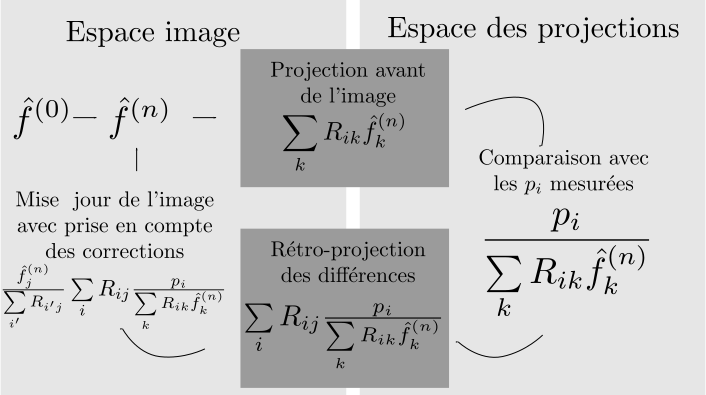
\includegraphics[width=12cm]{images/MLEM}
\caption[Schéma de principe de l'algorithme MLEM]{Schéma décrivant l'algorithme itératif ML-EM. $\hat{f}^{(n)}_j$ est l'estimation du voxel $j$ de l'image à l'itération $n$. $R_{ij}$ est la matrice système, et représente la probabilité de détecter une désintégration dans le voxel $j$ à la ligne de réponse $i$.}
\label{fig:schemaMLEM}
\end{figure}


	\subsection{Algorithme OS-EM (Ordered Subset Expectation Maximisation)}

L'algorithme OS-EM est une évolution de l'algorithme ML-EM  qui permet une accélération substantielle de la convergence en réalisant les itérations de l'équation~\ref{eq:MLEM} sur des sous-ensemble des données acquises~\cite{hudson1994accelerated}. 

Ces sous-ensembles de données sont réalisés en échantillonnant de manière régulière les lignes de réponses. Leur nombre est un des paramètres de l'algorithme, mais la convergence n'est plus garantit contrairement à ML-EM. En pratique, l'algorithme converge toujours approximativement, et le nombre d'itérations est déterminé de manière empirique~\cite{bailey2005positon}. Des évolutions de OS-EM ont été réalisées pour garantir une convergence, notamment l'algorithme Row-Action Maximum Likelihood (RAMLA)~\cite{browne1996row, chiang2004clinical}.

Le principal avantage de OS-EM est qu'il permet d'augmenter la vitesse de la reconstruction d'un facteur correspondant au nombre de sous-ensembles utilisés.

	\subsection{Cas des acquisitions en mode Séquentiel}
\label{lab:OPLEM}

Les acquisitions en mode séquentiel génèrent une suite d'enregistrements correspondant aux événements détectés par l'imageur. La lecture de tous ces événements un par un demande des temps de calculs extrêmement importants, c'est pourquoi Reader~\cite{reader2002one} ont proposé une adaptation de l'OS-EM au mode séquentiel appelée One-Pass List-Mode EM (OPL-EM). L'algorithme proposé est conçu pour ne parcourir qu'une seule fois la liste des événements. Comme pour OS-EM, les données sont groupées en sous-ensembles, qui sont utilisés les uns après les autres pour chaque itération, comme indiqué dans l'équation~\ref{eq:OSEM_seq}.

Ici, $s$ correspond à un numéro de sous-ensemble, $j$ à un voxel et $i$ à une ligne de réponse. Lorsque tous les sous-ensembles ont été parcourus, une nouvelle itération est déclenchée. Cet algorithme est conçu pour permettre de parcourir les données une seule fois, ce qui revient à réaliser une seule itération, cependant, il reste possible d'en réaliser plusieurs.

\begin{equation}
	f_j^{(s+1)}=\frac{\hat{f}_j^{(s)}}{\sum\limits_{i'}R_{i'j}}\sum\limits_{i \in T^s}R_{ij}\frac{1}{\sum\limits_{k}R_{ik}\hat{f}_k^{(s)}}
\label{eq:OSEM_seq}
\end{equation}

La différence entre OS-EM et cet algorithme est la manière dont sont sommées les différences. Dans OPL-EM, la sommation est réalisée sur l'ensemble des événements $T^n$ correspondant au sous-ensemble d'événements $n$. Cette somme est réalisée non pas pour chaque ligne de réponse $p$ comme précédemment, mais pour chaque événement détecté, ce qui explique le remplacement de $p_i$ par la valeur 1.
		
	\section{Reconstructions analytiques}

Ces algorithmes sont supplantés en oncologie par les algorithmes itératifs qui sont jugés plus performants sur l'évaluation du SUV et moins bruités~\cite{schoder2004clinical}.

Les méthodes analytiques utilisent la rétroprojection des projections du sinogramme pour reconstruire l'image. Si P est l'opération de projection d’une distribution $f(x,y)$ d’un objet vers $p(r, \theta)$, selon l’angle azimutal $\theta$, et $r$ la distance entre la projetée de la LDR dans le plan (x,y) et l’axe x, alors la projection peut s’écrire comme la transformée de Radon de cette distribution :

\begin{equation}
p(u, \theta) = P(f(x,y)) = \int\limits_{-\infty}^{+\infty} f(u~cos \theta - v~cos \theta, u~sin \theta + v~cos \theta) dv
\end{equation}

avec la relation suivante entre $(x,y)$ et $(u,v)$ :

\begin{equation}
	\begin{bmatrix}
	x \\
	y
	\end{bmatrix}
	=	
	\begin{bmatrix}
	\cos \theta &  - \sin \theta \\
	\sin \theta & \cos \theta
	\end{bmatrix}
	\quad
	\begin{bmatrix}
	u \\
	v
	\end{bmatrix}
\end{equation}

L'opération de rétroprojection notée RP approxime l'opération inverse de la projection et permet d'obtenir l'estimation $\hat{f}(x,y)$ en fonction des projections acquises :

\begin{equation}
\hat{f}(x,y) = RP(p(u, \theta))
\end{equation}

La rétroprojection simple consiste à ajouter les contributions de chaque ligne de réponse à l'image estimée :

\begin{equation}
\hat{f}(x,y) = \int\limits_0^\pi p(u, \theta)d\theta
\label{eq:nonFiltree}
\end{equation}


Cependant cette rétroprojection génère des artefacts en ``étoile'' autour de l'objet. La rétroprojection filtrée~\cite{kinahan1988three} permet de limiter ces artefacts. Elle est basée sur le théorème de la coupe centrale pour réaliser la rétroprojection des données. Ce théorème démontre que la transformée de Fourier  monodimensionnelle de la projection $p(u,\theta)$ selon la direction $\theta$ est égale à la transformée bidimensionnelle de la distribution $f(x,y)$ selon un plan perpendiculaire à la direction de projection et passant par l'origine :

\begin{equation}
\left[ TF_{2D}(f) \right](\upsilon_x, \upsilon_y) = \left[ TF_{2D}(b) \right](\upsilon_x, \upsilon_y)|\upsilon|
\end{equation}

avec b(x,y) correspondant au résultat de la rétroprojection non filtrée de l'équation~\ref{eq:nonFiltree}. 

Les projections mesurées sont d'abord filtrées par le filtre rampe $\upsilon$ dans le domaine de Fourier. On rétroprojète ensuite la transformée de Fourier inverse de ces données filtrées. On obtient alors l'estimation de la distribution originale $\hat{f}$.	
			
\part{Mouvement respiratoire}

	\chapter{Respiration et influence sur les acquisitions TEP/TDM}
	\section{Introduction}

Le mouvement respiratoire en imagerie TEP engendre plusieurs effets sur les images reconstruites, qui seront détaillés ci-après. Il occasionne notamment une diminution de la qualité des images, ce qui peut perturber le travail des praticiens. 

Nous ferons tout d'abord une introduction générale sur le mouvement respiratoire, puis nous enchaînerons ensuite sur les différents effets que peut avoir ce mouvement sur les images TEP, avec notamment des incertitudes sur la forme et la localisation des lésions et une diminution de l'activité estimée. Nous parlerons ensuite de l'impact de ce mouvement sur la détectabilité des lésions.

\section{Mouvement respiratoire}

Ce mouvement est la succession d'une phase inspiratoire, suivi d'une phase expiratoire. Chacune de ces phases combine plusieurs mouvements élémentaires~\cite{servant2007cours} :
 
\begin{enumerate}
 \item Thoracique, avec un déplacement des côtes.
 \item Abdominal, avec un déplacement du diaphragme.
 \item En cas d'inspiration forcée, action des pectoraux.
\end{enumerate}

La figure~\ref{fig:respiXCAT} représente 3 instants du cycle respiratoire utilisé dans le NCAT~\cite{segars2001These}, un modèle de corps humain respirant. On voit clairement tous les effets présentés précédemment, notamment le relèvement des côtes et du sternum par rapport aux guides de référence  présents sur les images.

\begin{figure}[h!]
    \begin{center}
            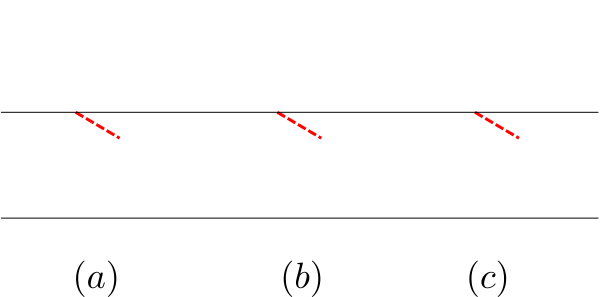
\includegraphics[width=10cm]{images/mvtRespi} \\
    \end{center}
    \caption[Modèle de mouvement intégré dans le fantôme NCAT]{Modèle de mouvement intégré dans le fantôme NCAT. La ligne pointillée rouge sert de référence pour la position d'une des côtes du modèle en expiration. L'image (a) correspond à l'expiration complète, et la (c) à la fin de l'inspiration. (b) correspond à un instant intermédiaire du cycle. }
    \label{fig:respiXCAT}
\end{figure}


La variabilité inter et intra-patient de ce mouvement est très importante : le volume d'air inspiré peut varier de 500 ml à 1200 ml selon que la personne a une respiration normale ou profonde. Pour ces deux extrêmes, la fréquence respiratoire varie de 5 cycles/min. à 20 cycles/min.~\cite{sherwood2006fundamentals}.

Or, une acquisition TEP a une durée de plusieurs minutes par lit, ce qui provoque des artefacts dû aux mouvements réalisés pendant l'acquisition, notamment au niveau de la localisation de la tumeur, de son activité mesurée et, par extension, de sa détection. De la même manière, des artefacts (voir figure~\ref{fig:artefactsCT}) apparaissent au niveau des zones de fort mouvement dans les images TDM, lorsque les organes bougent pendant une rotation du détecteur.

Nous allons tout d'abord introduire les effets visibles sur les images, puis nous nous attarderons sur les mesures quantitatives utilisées pour étudier l'apport de la correction du mouvement sur la détection des tumeurs. Enfin, nous dresserons un état de l'art plus précis des publications s'intéressant à l'impact du mouvement respiratoire sur la détection.

\section{Localisation et volume}


La localisation et le volume apparent des tumeurs sur les images TEP peuvent être modifiés par le mouvement engendré par la respiration (voir figure~\ref{fig:effetMvt}). D'après l'étude de~\cite{lamare2007respiratory}, réalisée sur des simulations Monte-Carlo à l'aide du logiciel de simulation GATE~\cite{jan2004gate} en utilisant le modèle NCAT~\cite{segars2001These}, la largeur à mi-hauteur des lésions peut être modifiée de 48\% (équation~\ref{eq:PRD} : Différence relative) dans le cas d'une lésion de 7mm de diamètre dans la partie basse du poumon. L'imprécision axiale sur le positionnement de la tumeur peut atteindre 9\% dans les mêmes conditions.

\begin{equation}
\%DR= \left| \frac{Crit\grave{e}re~sur~image~non~corrig\acute{e}e - Crit\grave{e}re~sur~image~de~r\acute{e}f\acute{e}rence}{Crit\grave{e}re sur image~de~r\acute{e}f\acute{e}rence} \right|
\label{eq:PRD}
\end{equation}


\begin{figure}[h!]
    \begin{center}
            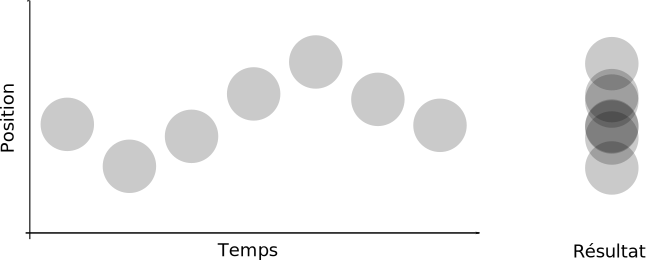
\includegraphics[width=10cm]{images/moyennageImage} \\
    \end{center}
    \caption[Effet du déplacement d'une tumeur sur les données acquises]{Effet du déplacement d'une tumeur sur les données acquises. La position de la tumeur change en fonction du temps, ce qui provoque l'acquisition d'une tumeur équivalente présentée à droite.}
    \label{fig:effetMvt}
\end{figure}


\section{Mesure de l'activité des tumeurs}

Le contraste des tumeurs par rapport au fond est un critère important pour déterminer la malignité des tumeurs~\cite{dimitrakopoulou2002role, krak2005effects}. De plus ce contraste joue aussi un rôle important sur la détectabilité de la tumeur en facilitant sa distinction du fond, comme nous allons le voir ci-après.

L'activité peut être influencée par la respiration de deux manières : 
\begin{itemize}
 \item Par un mauvais ajustement de la carte d'atténuation.
 \item Par le moyennage de la position de la tumeur.
\end{itemize}


\subsection{Décalage de la carte d'atténuation}

La carte d'atténuation utilisée pour corriger les images d'émission est basée sur une image TDM prise à un instant donné du cycle. Or l'atténuation de la zone correspondant à une tumeur peut être différente de celle des tissus environnants, ce qui peut occasionner des sous-estimations ou des sur-estimations de l'activité de la tumeur si la carte d'atténuation est mal positionnée.

D'après l'étude~\cite{erdi2004ct}, on peut observer des variations très importantes de $SUV_{max}$ (voir équation~\ref{eq:varSUV}) sur les images TEP reconstruites. L'étude a été réalisée sur 5 patients totalisant 8 lésions. L'acquisition TDM 4D a été synchronisée sur le mouvement à l'aide d'un dispositif placé sur l'abdomen du patient. Ce dispositif était constitué de deux marqueurs réfléchissant les ondes infrarouges, placés dans le champ de vue d'une caméra. Les données synchronisées acquises en TDM 4D ont été utilisées pour générer un cycle de 10 images TDM. Chacune de ces 10 images a ensuite servi de carte d'atténuation lors de la reconstruction des images d'émission, générant ainsi 10 images TEP .

\begin{equation}
\label{eq:varSUV}
 \%~variation~SUV_{max} = 100 \times \frac{ | SUV_1 - SUV_2 | }{ (SUV_1 + SUV_2) / 2 }
\end{equation}


Les données TEP reconstruites à partir des 10 images ont montré de grandes différences en terme de SUV selon l'instant du cycle à partir duquel les lésions ont été extraites.
Ces variations allant jusqu'à 24\% pour une lésion de $19.8~mm^3$ placée dans l'espace médiastinal, entre une reconstruction TEP réalisée à partir d'une image TDM de fin d'expiration et une image TDM de fin d'expiration. En recherchant la variation la plus grande sur l'ensemble du cycle (en non pas en se limitant aux extrêmes), la variation peut atteindre 30\%.

La figure~\ref{fig:lesionEnFctPhaseTDM} présente la variation de $SUV_{max}$ en fonction de la phase utilisée pour la reconstruction.


\begin{figure}[h!]
	\vspace{0.5cm}
	\centering
			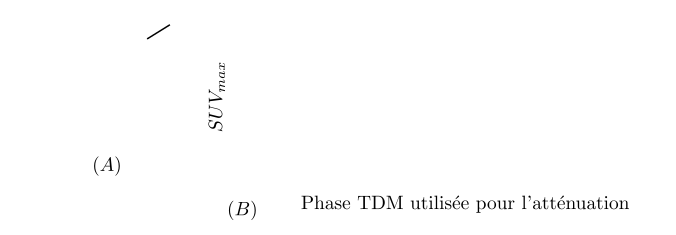
\includegraphics[width=12cm]{images/lesionEnFctPhaseTDM}
	\vspace{-0.5cm}
	\caption[Influence de l'influence de la carte d'atténuation sur l'activité des lésions] {A) Vue coronale d'un patient avec une lésion clairement visible en haut à droite (flèche noire).  B) $SUV_{max}$ observé sur les images reconstruites en fonction de l'image TDM utilisée pour la reconstruction. Le nombre en abscisse représente la position dans le cycle respiratoire en pourcentage.} 
	\label{fig:lesionEnFctPhaseTDM}
\end{figure}

\subsection{Artefacts TEP dus aux artefacts TDM}

On peut voir sur les images de la figure~\ref{fig:artefactsCT} des artefacts présents sur les images TDM utilisées pour la correction d'atténuation. Ces artefacts proviennent de la manière dont les images sont acquises : le couple ``source de rayons X-détecteur'' tourne autour du sujet dans un mouvement hélicoïdal, et l'algorithme de reconstruction va ensuite utiliser les acquisitions pour reconstruire une image complète. Or, en cas de respiration rapide, des incohérences peuvent survenir quand le mouvement du diaphragme est plus important que celui de la caméra. Ce type d'artefacts peut créer des incohérences dans les images TEP reconstruites, car le poumon sera corrigé de l'atténuation avec des coefficients non uniformes.

\begin{figure}[h!]
	\begin{center}
		\begin{tabular}{c c}
			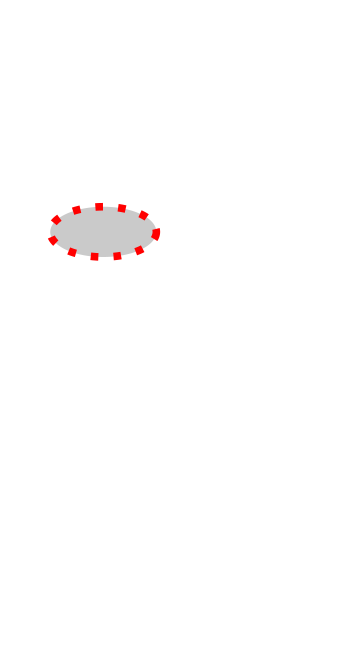
\includegraphics[width=5cm]{images/artefactCT1} & 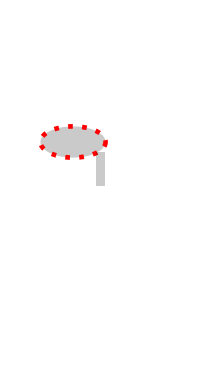
\includegraphics[width=5cm]{images/artefactCT2}
		\end{tabular}
	\end{center}
	\caption{Artefacts présents sur des images TDM utilisées pour la correction d'atténuation.} 
	\label{fig:artefactsCT}
\end{figure}


\subsection{Déplacement de la tumeur au cours du cycle}

Le mouvement respiratoire va avoir pour effet de déplacer la tumeur pendant l'acquisition, ce qui va moyenner la quantité de radioactivité sur l'ensemble du cycle, comme indiqué sur la figure~\ref{fig:effetMvt}. Si le déplacement de la tumeur est suffisamment grand par rapport à son diamètre, la réduction de radioactivité va être importante.

L'étude~\cite{boucher2004respiratory} réalisée sur un fantôme elliptique (modèle ``Elliptical Jaszczak Phantom'') montre qu'un déplacement d'une source radioactive de 6 mm sur un cycle respiratoire moyen entraîne une sous-estimation de l'activité maximale de la source de 41\% pour un objet de 1.2 ml et de 21\% pour une sphère de 19.4 ml.


\section{Impact du mouvement respiratoire sur la détection}

Peu de travaux ont été réalisés sur l'impact du mouvement respiratoire sur la détection des tumeurs. Globalement, les publications traitent  principalement de la mesure de la quantification des lésions ($SUV_{max}$, profils de lésions, ...). Très peu d'articles utilisent des critères orientés sur les performances de détection.

Voici une liste des critères utilisés dans différentes publications pour évaluer les performances d'algorithmes de correction du mouvement respiratoire :

\begin{enumerate}
 \item Basés sur la récupération de l'activité des lésions, $SUV_{max}$, contraste :~\cite{GuopingChang2010Implementation,lamare2007list,nehmeh2002effect,detorie2008quantitative}.
 \item Sur la visualisation des profils de lésion :~\cite{GuopingChang2010Implementation,Thielemans2006Lesion,lamare2007list}.
 \item Sur la récupération du volume et de la position de la lésion :~\cite{GuopingChang2010Implementation,lamare2007list,nehmeh2002effect}.
 \item Sur le rapport signal sur bruit (SNR) :~\cite{GuopingChang2010Implementation}.
 \item Sur l'observateur de Hotelling (CHO) :~\cite{Thielemans2006Lesion}.
\end{enumerate}

Comme on peut le voir, les deux seuls critères qui pourraient s'approcher d'une étude sur la détection sont le SNR et le CHO, mais ils sont largement sous-représentés. 

Je vais me concentrer sur les deux publications the Thielemans et Chang qui utilisent un observateur.

Un autre document par Rahmim Arman~\cite{rahmim4d} propose d'utiliser le CHO pour évaluer l'amélioration de la détection des défauts dans de l'imagerie cardiaque corrigée du mouvement respiratoire. Ce document n'a pas encore donné lieu à publication.
	
\subsection{Article de Thielemans et al.~\cite{Thielemans2006Lesion}}
\label{lab:articleThielPres}
Dans sa publication, Thielemans et al. utilisent le ``Channelized Hotelling Observer'' (CHO)~\cite{barrett1993model}, qui est un observateur dérivé du classifieur linéaire LDA présenté en \ref{lab:LDA}, utilisé en conjonction avec des informations fréquentielles. 

L'étude se base sur des simulations analytiques d'un fantôme thoracique dans lequel sont insérées des lésions sphériques de gros diamètre (13 mm) et de contraste élevé (4.25:1). Cette étude qui compare plusieurs méthodes de correction du mouvement respiratoire est détaillée dans le chapitre suivant en~\ref{lab:evolGating}.
%
%Cependant ils n'utilisent le CHO que sur des lésions de forts diamètre et de fort contraste (13mm de diamètre et contraste de 4.25:1).


%Les résultats présentés (figure~\ref{fig:apportCHO}) montrent une amélioration du score pour les méthodes de correction de l'ordre de 50\% dans certains cas. 

%Mais il est difficile d'évaluer de manière précise l'apport des méthodes de détection à l'aide de ces seuls ``scores'' car ce sont des résultats qualitatifs. 



\subsection{Article de Chang et al.~\cite{GuopingChang2010Implementation}}

Cette publication est une évaluation clinique d'un système de découpage automatique du signal respiratoire selon l'amplitude. Elle est basée sur 13 patients totalisant 21 tumeurs du poumon de taille diverses (estimée de 1 à 27 cm$^3$. Le signal respiratoire est acquis à l'aide d'un dispositif propriétaire (Anzai AZ-733V) basé sur une ceinture abdominale avec capteur de pression. Seules les données TEP acquises autour d'une amplitude présélectionnée (+/-10\% de l'amplitude correspondant à l'acquisition TDM) sont utilisées pour la reconstruction des images corrigées. 

Le jeu d'images ``témoin'', non corrigées, est réalisé en extrayant des données acquises le même nombre d'évènements N que le jeu d'images synchronisées en considérant les N premiers du fichier en mode séquentiel.

L'auteur compare le $SUV_{max}$, $SUV_{moyen}$, Rapport Signal/Bruit (SNR) et volume apparent de la lésion pour les deux jeux d'images. Le volume de la lésion et le $SUV _{moyen}$ sont calculés sur une région d'intérêt correspondant à 40\% du $SUV_{max}$ de la lésion. Le SNR est calculé en divisant le SUV moyen de la tumeur par l'écart-type d'une zone d'intérêt dans le poumon, dont ni la taille ni la localisation ne sont précisées. 

Les résultats présentés montrent une amélioration importante des valeurs du SNR pour les images corrigées du mouvement par rapport aux images témoin, comme présenté dans la figure~\ref{fig:guoping2010Exemple}. En moyenne, cette augmentation est de 26.3\%, mais deux tumeurs sur les 21 de l'étude voient leur SNR augmenter de plus de 66\%. 

\begin{figure}[h!]
	\centering
			\includegraphics[width=10cm]{images/guoping2010Exemple}
	\caption{Exemple d'image avec et sans correction de mouvement respiratoire.} 
	\label{fig:guoping2010Exemple}
\end{figure}




Il est étonnant de constater que les mesures moyennes sur les 21 tumeurs de $SUV_{max}$ et $SUV_{moyen}$ voient leurs valeurs augmenter respectivement de 26.8\% et 26\%, ce qui est tout à fait semblable avec l'augmentation de SNR. Cependant, les valeurs individuelles d'amélioration  pour chaque tumeur ne montrent pas de corrélation avec le SNR. Par exemple, une lésion va montrer une augmentation de 24\% de son $SUV_{max}$, de 20\% de son $SUV_{moyen}$ et de 37\% de son SNR.

Il est intéressant de constater qu'il y a un point où le SNR diminue de 3.4\%, mais que le $SUV_{max}$ et le $SUV_{moyen}$ augmentent tout de même de presque 18\%. Cela semble indiquer une erreur car le SUV de la zone d'intérêt n'est pas censé changer de manière importante.

	
	\chapter{Processus d'estimation du mouvement}
	\section{Introduction}

Cette partie présente tout d'abord la problématique du mouvement respiratoire en TEP. Puis il aborde successivement les différentes techniques permettant d'estimer soit le signal respiratoire, soit le champ de mouvement 3D des organes internes du patient. Enfin, le dernier chapitre montre comment cette information sur le signal respiratoire ou le champ de mouvement peut être prise en compte pour corriger les phénomènes de dégradation engendrés par la respiration.


\section{Estimation du signal respiratoire}

Le signal respiratoire est une grandeur caractérisant la position du patient sur le cycle respiratoire, entre la fin d'inspiration et la fin d'expiration. Il est habituellement fourni par des capteurs externes qui génèrent un signal corrélé avec la respiration. Cela permet de faire correspondre les données acquises par un imageur avec une phase particulière du mouvement respiratoire.

\subsection{Spiromètre}
\label{lab:spirometre}
Le spiromètre est un capteur externe placé sur la bouche du patient et qui permet de mesurer les déplacements d'air dans le système respiratoire~\cite{guivarc2004synchronization}. Les spiromètres mesurent un débit ou un volume d'air inspiré/expiré (voir illustration figure~\ref{fig:spirometre}). \`A partir de l'une des grandeurs (volume ou débit), il est possible d'estimer l'autre facilement. L'avantage du spiromètre est qu'il permet d'accéder à une mesure caractérisant directement la respiration du patient, et n'est pas sujet à des perturbations externes (mouvements involontaires par exemple). Par contre cela demande un appareillage qui peut être assez invasif pour le patient.

\begin{figure}[h!]
	\begin{center}
		\includegraphics[width=12cm]{images/spiro}
	\end{center}
	\caption[Illustration du spiromètre Syn'r]{Illustration du spiromètre Syn'r : on peut voir le système de mesure de la respiration ainsi qu'un système de moniteurs implantés dans les lunettes pour aider le patient à contrôler sa respiration.} 
	\label{fig:spirometre}
\end{figure}

\subsection{Ceinture}

Pour mesurer le signal respiratoire, il est possible d'utiliser un capteur qui va mesurer le périmètre du thorax. L'extension de cette ceinture va correspondre aux mouvements de la cage thoracique et de l'abdomen pendant la respiration du patient. C'est une mesure indirecte de l'amplitude du mouvement respiratoire utilisée couramment en routine clinique. 

Différentes technologies existent pour mesurer cette information (RespiTrace R250 de Studley. Data Systems, Respiratory Belt Transducer de ADInstruments, ...). Elles sont basées sur plusieurs effets (résisitif, inductif...) et ont l'avantage d'avoir un faible coût et de ne pas perturber le patient.

Bien qu'elles puissent être influencées par les mouvements involontaires du patient, il a été montré dans~\cite{Guivarch2004Sync} que les données acquises selon les méthodes par respiromètre et par ceinture sont équivalentes.

\subsection{Techniques basés sur des caméras vidéo}

Des caméras peuvent être utilisées pour estimer le mouvement respiratoire. Une des techniques consiste à utiliser des informations surfaciques en reconstruisant en 3D certaines parties du corps à l'aide de plusieurs caméras~\cite{beach2004feasibility}, ou en utilisant des caméras 3D temps de vol~\cite{fayad2009patient}. Cela permet d'avoir plus d'informations sur la respiration.

Une autre technique consiste à installer un marqueur sur le corps du patient et à relever les déplacements de ce marqueur selon plusieurs axes à l'aide d'une ou plusieurs caméras. Un tel système est décrit dans~\cite{nehmeh2002effect}. L'un de ces systèmes, le ``Respiratory Gating System'' de Varian Medical Systems est illustré sur  la figure~\ref{fig:RGSdeVarian}.

\begin{figure}[h!]
	\begin{center}
		\includegraphics[width=12cm]{images/varian}
	\end{center}
	\caption[Photographie du système RGS de Varian medical Systems en action]{Photographie du système RGS de Varian medical Systems en action : une caméra va détecter le déplacement d'une zone du thorax en mesurant le déplacement de marqueurs placés sur un bloc plastique.} 
	\label{fig:RGSdeVarian}
\end{figure}

Ces techniques ont l'avantage d'être moins invasives et plus facilement acceptées par le patient. Cependant, elles sont beaucoup plus sensibles aux mouvements involontaires du patient. Ce risque est faible pour l'imagerie TDM car de faible durée (inférieure à la minute), mais il devient important pour les acquisitions TEP qui peuvent durer en tout plusieurs dizaines de minutes. Ces mouvements n'étant probablement pas corrélés avec le mouvement respiratoire, ils vont perturber le signal obtenu. 

\subsection{Techniques basées sur les images TEP}
\label{lab:estimMvtTEP}
En TEP, la publication de Bundschuh et al.~\cite{bundschuh2007postacquisition} utilise les données dynamiques pour estimer le signal respiratoire sans avoir besoin de capteur externe. Ce processus est réalisé en 5 étapes : 

\begin{enumerate}
 \item Les données TEP sont acquises en mode séquence (aussi appelé mode liste, défini en \ref{lab:modeliste}) : toutes les désintégrations détectées sont enregistrées dans un fichier de manière séquentielle.
 \item Une image TEP statique est reconstruite. Elle permet de localiser une lésion dans l'image qui servira d'amer pour l'estimation du mouvement respiratoire.
 \item Les données dynamiques sont regroupées en blocs de 0.5 secondes d'acquisitions. Chaque bloc est reconstruit séparément. 
 \item La zone d'intérêt choisie précédemment est sélectionnée dans chaque image reconstruite. La position axiale du barycentre à chaque instant temporel va donner une estimation du mouvement respiratoire pour le volume donné.
\end{enumerate}

Cette technique a été évaluée sur 10 patients et les signaux ont été comparés avec ceux obtenus avec des ceintures abdominales. Pour 3 patients, les courbes respiratoires obtenues par les deux techniques étaient très fortement corrélées. Pour deux autres patients, l'estimation de mouvement obtenue par la TEP était trop bruitée, mais montrait une bonne corrélation avec le signal obtenu par les ceintures abdominales après filtrage. Pour 3 autres patients, il n'a pas été possible de trouver une corrélation entre les deux signaux. Les deux derniers patients ont bougé pendant l'acquisition TEP, ce qui a perturbé le signal.

Cette technique est intéressante mais contrainte par la qualité de l'image TEP. En pratique, la moitié des acquisitions TEP n'a pas permis d'obtenir un signal respiratoire satisfaisant.


\section{Estimation du champ de mouvement}
\label{lab:estimChamp}

Le champ de mouvement est une information beaucoup plus riche que le signal respiratoire car il permet de suivre les déplacements des organes et des lésions à l'intérieur du corps du patient au cours d'un cycle respiratoire.

Le signal respiratoire acquis par les méthodes précédemment citées est utilisé pour décomposer les données acquises en TDM ou TEP en plusieurs phases, chacune correspondant à un instant du cycle. Ces informations sont utilisées pour rassembler les données acquises lors de chaque phase, reconstruites indépendamment. Ces reconstructions vont être utilisées pour estimer le champ de mouvement à l'aide de techniques de recalage.


\subsection{Image TEP 4D}
\label{lab:estimMvtTEP4D}
L'estimation du champ de mouvement respiratoire peut être faite à partir des données TEP, comme il a été montré par~\cite{dawood2008respiratory, dawood2006lung}. 

Les techniques utilisées sont analogues à celle présentée en~\ref{lab:estimMvtTEP}. Elles consistent à réaliser une acquisition séquentielle des données en même temps qu'une acquisition du signal respiratoire, puis à réorganiser les données acquises pour reconstruire les différents instants du cycle indépendamment et sans correction d'atténuation. Le mouvement est ensuite estimé à partir de ces images.

Pour obtenir le signal respiratoire, Dawood~\cite{dawood2008respiratory} utilise une caméra vidéo qui enregistre le mouvement d'un marqueur placé sur l'abdomen du patient. Ce marqueur est un point blanc placé sur un disque noir, et sa position axiale est détectée en calculant le barycentre des pixels dépassant un certain seuil. 

La synchronisation avec l'acquisition PET est réalisée à l'aide d'une LED située dans le champ de vue de la caméra qui s'allume lors du début de l'acquisition. Une fois l'acquisition terminée, le signal respiratoire obtenu par la caméra est utilisé pour répartir les évènements acquis par l'imageur TEP le long du cycle respiratoire. Ce cycle est décomposé en 8 parties qui seront reconstruites séparément, sans correction d'atténuation.

Les auteurs utilisent ensuite un algorithme de flux optique 3D présenté dans~\cite{dawood2006lung} et~\cite{horn1981determining} pour déterminer le champ de mouvement : Ils estiment un déplacement entre chaque image du cycle et l'image de référence correspondant à la quatrième phase (mi-expiration) dans le cas de cet article. Le résultat de l'algorithme est donc une séquence de champ de mouvement 3D,  formant un champ de déformation 4D.

L'algorithme a été testé sur le fantôme XCAT~\cite{segars2009mcatoverview} ainsi que sur les données de 16 patients. La performance de l'estimation de mouvement a été évaluée selon trois critères sur les images corrigées : la correction du déplacement axial du coeur, le coefficient de corrélation des images corrigées du mouvement, ainsi que le bruit obtenu. Ces résultats sont détaillés dans la présentation de cet article de la partie~\ref{lab:correctionDawood2008}.

Bai a présenté une technique d'estimation semblable~\cite{bai2009regularized}. L'étude a été réalisée sur des images simulées à l'aide du logiciel PET-SORTEO~\cite{reilhac2005pet} en utilisant le modèle NCAT~\cite{segars2009mcatoverview}, ainsi que sur une acquisition clinique. 24 lésions de forts contrastes (8:1) ont été introduites dans les modèles, pour une durée d'examen simulé de 10 minutes. L'erreur moyenne du diamètre longitudinal des lésions est très fortement améliorée par la correction, avec une erreur passant de 36\% à 16\% en moyenne sur l'ensemble des lésions. Le principe est le même que pour la publication précédente, à la différence que l'estimation de mouvement a été réalisée sur des images corrigées de l'atténuation à partir de la carte d'atténuation de la phase de référence. De plus, cette estimation du mouvement à été réalisée à l'aide d'une interpolation par B-splines~\cite{thevenaz2000optimization}.

Un exemple de champ de déformation obtenu sur l'acquisition clinique est présenté en~\ref{fig:champMouvementBai}

\begin{figure}[h!]
	\begin{center}
		\includegraphics[width=12cm]{images/champDeformBai2}
	\end{center}
	\caption[Exemple de champ de mouvement]{Champ de déformation calculé sur des données cliniques à l'aide de la méthode présenté dans~\cite{bai2009regularized}. a) Image TEP obtenue à partir des données de la phase de référence  (mi-expiration), b) Image reconstruite pour les données d'expiration complète, et c) Résultat du recalage de l'image de fin d'expiration sur l'image de référence. d) représente le champ de mouvement résultat. Les traits rouges représentent l'extension axiale de la tumeur dans l'image de référence.} 
	\label{fig:champMouvementBai}
\end{figure}

\subsection{Image TDM 4D}

Les images TDM peuvent être acquises en mode dynamique de manière à obtenir une suite d'images couvrant tout le cycle respiratoire~\cite{lamare2007list, qiao2006motion}. Les données sont reconstruites indépendamment, avec un rapport signal sur bruit plus faible que sur l'image originale. 

Des algorithmes de recalage sont utilisés de manière à déduire le champ de mouvement. Le principal avantage de l'utilisation des images TDM 4D par rapport à la TEP est la précision des images. En effet, alors que les images TEP ont une résolution de l'ordre de 5mm, les images TDM atteignent des résolutions inférieures au mm, ce qui permet d'obtenir un champ de mouvement beaucoup plus précis. Cependant, utiliser des images TDM 4D a plusieurs inconvénients :

\begin{itemize}
 \item Une possible incohérence entre le cycle acquis en TDM 4D et la respiration du patient en TEP. Bien que les imageurs TEP/TDM couplent les deux sur la même machine, de manière à éviter les mouvements du patient entre les acquisitions, le cycle acquis en TDM ne représente qu'un cycle, tandis que l'acquisition TEP va donner un ``cycle moyen`` plus proche de la réalité.
 \item Une dose de radiation émise plus importante. Bien que les technologies récentes permettent de réduire les doses de manière importante pour l'acquisition dynamique, elles restent tout de même plus importantes que pour un CT 3D.
\end{itemize}

Il faut noter que plusieurs publications basées sur des simulations se servent des cartes de labels utilisées par le simulateur pour réaliser les estimation de mouvement~\cite{lamare2007list}. Cela donne une estimation dans le ``meilleur des cas'', où l'image TDM est parfaitement en phase avec les images TEP. On utilise alors la méthode décrite précédemment pour estimer le champ de mouvement. L'intérêt de cette méthode est que les données anatomiques sont moins bruitées que les données TEP et contiennent plus d'information pour l'estimation des déformations. Cependant, l'acquisition d'un scanner TDM 4D en routine clinique peut être considérée comme très irradiante.

\subsection{Modèle}

Une autre voie en cours de développement est basée sur la création d'un modèle de respiration qui est adapté à chaque patient à partir d'une quantité réduite de données. Fayad~\cite{fayad2010application} propose un modèle basée sur l'analyse en composantes principales du champ de mouvement. 

Ce modèle est adapté à un patient à partir de deux images TDM prises à des instants différents du cycle, et d'un maillage dynamique de la surface du corps du patient obtenu pendant un cycle respiratoire complet. Dans son implémentation, le maillage est obtenu à l'aide d'une caméra vidéo temps de vol.

L'avantage de ce modèle est qu'il est totalement continu, et permet l'extraction d'un nombre arbitraire de phases sous la forme de matrices de déformation. Ce modèle a été testé sur des images simulées (2 fantômes XCAT) et 6 patients.

L'article \cite{vandemeulebroucke2009respiratory} présente une autre technique adaptée à l'imagerie TDM. Dans ce cas, un modèle est généré à partir d'une acquisition TDM 4D en créant une image de mouvement moyenne, puis ce modèle est utilisé pour déduire le mouvement interne à partir d'acquisition de fluoroscopies en temps réel.
	
	\chapter{Correction du mouvement respiratoire}
	\label{lab:corrMvt}

\section{Introduction}

Nous allons maintenant présenter les techniques de correction du mouvement respiratoire proposées dans la littérature. 

Deux approches existent pour la correction du mouvement : les techniques dites prospectives, qui consistent à réaliser la correction pendant l'acquisition en sélectionnant les données à conserver, et rétrospectives, qui réalisent la correction \textit{a posteriori}, après l'acquisition des données. Actuellement, les techniques les plus prometteuses sont rétrospectives, car elles permettent d'utiliser l'ensemble des données du cycle respiratoire.

\section{Synchronisation respiratoire}

La synchronisation respiratoire correspond à un découpage du cycle respiratoire selon la phase (voir figure~\ref{fig:gatingRespi}) ou l'amplitude (voir figure~\ref{fig:gatingRespiAmplitude}). Une seule des phases ou amplitude sera sélectionnée pour la reconstruction. En théorie cela permet d'avoir le meilleur résultat, car il est possible de sélectionner les événements correspondants à la phase ou l'amplitude où a été acquise la carte d'atténuation.


\begin{figure}[h!]
	\begin{center}
		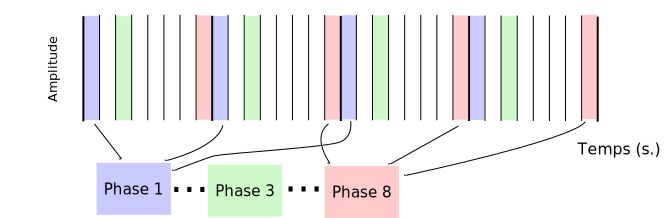
\includegraphics[width=14cm]{images/ET-IM}
	\end{center}
	\caption[Illustration de la synchronisation respiratoire en phase]{Illustration de la synchronisation respiratoire en phase : Le cycle respiratoire acquis est découpé selon la position du signal acquis dans le cycle. Le signal est analysé pour déterminer les débuts et fins de cycles. Chaque cycle est découpé en un nombre déterminé de phases égales.} 
	\label{fig:gatingRespi}
\end{figure}


\begin{figure}[h!]
	\begin{center}
		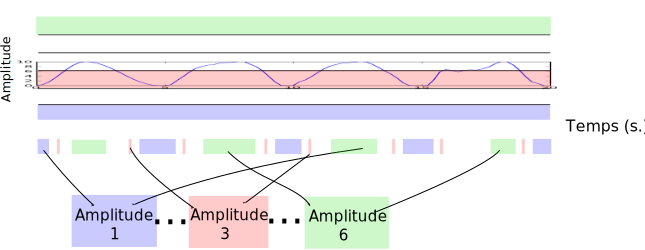
\includegraphics[width=14cm]{images/gatingAmplitude}
	\end{center}
	\caption{Illustration de la synchronisation respiratoire en amplitude : Le cycle respiratoire acquis est découpé selon son amplitude.} 
	\label{fig:gatingRespiAmplitude}
\end{figure}


Cette technique est notamment présentée dans~\cite{nehmeh2002effect}, où le signal respiratoire est estimé par une caméra qui suit un marqueur placé sur le torse du patient (système RPM de Varian Medical Systems). L'étude a été réalisée sur 5 patients volontaires comme suit : un scan de transmission de 3 minutes, suivi d'une acquisition avec correction de 10 minutes, puis d'une acquisition témoin non corrigée de 3 minutes. La décomposition du cycle s'effectue en fonction de la phase. L'auteur annonce une amélioration de l'estimation du volume des tumeurs pouvant aller jusqu'à 34\%, avec une augmentation du $SUV_{max}$ de 160\%. 

Une autre publication~\cite{boucher2004respiratory} utilise un thermomètre détectant l'air chaud émis en début de cycle respiratoire pour réaliser la synchronisation. Les différentes reconstructions issues de l'expérience sont visibles sur la figure~\ref{fig:boucher2004}. Il faut noter que la partie clinique de cette étude a été réalisée sur 10 patients sains, et qu'il n'y a donc pas de mesures de performance de la correction du mouvement sur les lésions. 

\begin{figure}[h!]
	\begin{center}
		\includegraphics[width=12cm]{images/gatingBoucher2004}
	\end{center}
	\caption[Illustration de l'étendue du mouvement respiratoire sur des images reconstruites ]{Illustration de l'étendue du mouvement respiratoire sur des images reconstruites après synchronisation respiratoire~\cite{boucher2004respiratory}. La rangée du haut montre l'étendue du mouvement de l'apex du coeur, et celle du bas l'étendue du mouvement du rein} 
	\label{fig:boucher2004}
\end{figure}

Une variante de cette technique ne nécessitant pas de capteur est décrite dans~\cite{nehmeh2003reduction}. Un point faiblement radioactif est fixé au-dessus du torse du patient. Les acquisitions de l'imageur sont ensuite enregistrées par blocs temporels de 1 seconde, et une zone d'intérêt est reconstruite dans chacune des images. Les données reconstruites montrant le point source dans cette zone d'intérêt sont sommées et l'image finale reconstruite. 

Cette technique a été comparée avec celle présentée précédemment~\cite{nehmeh2002effect} basée sur le système RPM de Variant. Ces deux techniques n'ont été testées cliniquement que sur un patient mais ont montré des performances tout à fait semblables (6\% de différence dans les activités et 2\% pour le volume de la lésion).

Cependant, ces techniques n'utilisent pas forcément une carte d'atténuation optimisée pour la position du cycle correspondant aux acquisitions TEP. L'article~\cite{boucher2004respiratory} utilise par exemple une carte d'atténuation obtenue par transmission, qui est est une moyenne acquise sur plusieurs cycles respiratoire. Chang et al.~\cite{GuopingChang2010Implementation} estiment la carte d'atténuation à partir d'une image TDM réalisée en respiration libre synchronisée. La phase du cycle respiratoire où l'acquistion TDM a été réalisée est enregistrée, et les données TEP acquises sur tous les cycles à cette phase sont reconstruites (voir exemples figure~\ref{fig:chang2010}). Les résultats présentés sur 13 patients (21 tumeurs) montrent une amélioration du rapport signal sur bruit pouvant aller de -3.4 à 81\% suivant les tumeurs, avec une amélioration moyenne de 26.3\%.

\begin{figure}[h!]
	\begin{center}
		\begin{tabular}{c c}
			\includegraphics[width=10cm]{images/chang2010}
		\end{tabular}
	\end{center}
	\caption[Images TEP/TDM superposées du poumon]{Images TEP/TDM superposées du poumon reconstruites avec et sans synchronisation respiratoire en utilisant la méthode décrite dans~\cite{GuopingChang2010Implementation}. On peut observer que les tumeurs sont mieux définies et correspondent à l'image TDM qui sert de référence.} 
	\label{fig:chang2010}
\end{figure}

L'inconvénient majeur de ces techniques est qu'elles demandent un temps d'acquisition beaucoup plus long à qualité d'image égale. Si l'on ne conserve que 20\% des évènements détectés, cela signifie qu'il faut augmenter le temps d'acquisition d'un facteur 5 pour obtenir une image de qualité égale. Il n'est donc pas envisageable de mettre en place ces protocoles en routine clinique, car le temps disponible n'est pas suffisant. C'est pour cela que de nombreuses équipes se sont mises à travailler sur une évolution de cette technique, où les images sont acquises en mode synchronisé  puis recalées et sommées pour prendre en compte toute la statique.

\section{Synchronisation respiratoire avec recalage}
\label{lab:corrPostRecon}

Dans cette section, nous allons détailler la technique consistant à corriger le mouvement en recalant les images reconstruites de chaque phase du cycle respiratoire.

Ces techniques se basent toutes sur une estimation préalable du mouvement respiratoire. Les images de chaque phase sont reconstruites indépendamment, puis recalées sur une phase de référence grâce au champ de mouvement. Enfin, les images déformées sont sommées. La difficulté principale se situe dans l'estimation du champ de mouvement interne lors de la respiration, car ce mouvement est complexe.

Les premières publications décrivant cette technique l'utilisaient notamment pour réaliser de l'imagerie cardiaque en TEP~\cite{klein19973d}. Cette publication démontre la faisabilité du procédé sur un animal en utilisant des techniques de flux optique pour estimer le champ de mouvement. En effet le coeur a l'avantage d'avoir une activité métabolique intense, ce qui rend l'estimation de son mouvement relativement aisée même sur des images avec une faible statistique.




\subsection{Estimation du mouvement respiratoire corps entier}

L'estimation du champ de mouvement interne se fait à l'aide d'une des méthode présentées précédemment en~\ref{lab:estimChamp} et rappelée brièvement :

\subsubsection{Imagerie TEP avec synchronisation respiratoire}
\label{lab:correctionDawood2008}

L'acquisition TEP est réalisée en même temps que l'acquisition du signal respiratoire. Une image est reconstruite par phase du signal respiratoire, puis un algorithme d'estimation de mouvement est utilisé pour calculer le champ de mouvement entre les instants du cycle.

Les premiers algorithmes étaient utilisés en imagerie cardiaque~\cite{klein2002four} avec des transformations simples (affines), puis d'autres algorithmes plus adaptés aux images corps entier ont été utilisés, comme les flux optiques~\cite{dawood2006lung, dawood2006lung}, ou l'interpolation par B-spline~\cite{bai2009regularized}. 


\subsubsection{Imagerie CT 4D}

Les images CT 4D peuvent être utilisées pour réaliser l'estimation du mouvement respiratoire au lieu des données TEP. Cela nécessite un temps d'acquisition plus long et augmente la dose d'irradiation reçue par le patient.
Dawood a réalisé plusieurs publications sur le sujet en utilisant le flux optique pour l'estimation du champ de mouvement~\cite{dawood2006lung, dawood2008respiratory}. L'algorithme a été étudié sur des images de patients réels. Une autre publication~\cite{thorndyke2006reducing} indique une amélioration du rapport de contraste sur bruit (CNR) d'un facteur 3 grâce à la correction.


\section{Correction pré-reconstruction}

Les méthodes de correction du mouvement pré-reconstruction modifient les positions des lignes de réponse (LDR) estimée par l'imageur TEP.
Ce recalage des LDR correspond à un déplacement des lignes de réponse dans l'espace du détecteur (voir figure~\ref{fig:recalageLOR}) en fonction du mouvement respiratoire. La limitation principale de ce type de méthode est que le champ de mouvement ne peut pas être élastique.

Cependant, il a été étudié en imagerie du cerveau~\cite{bloomfield2003design}, où il permettait de corriger les mouvements de la tête. Il a été aussi utilisé en imagerie cardiaque TEP~\cite{livieratos2005rigid} en utilisant un champ de mouvement rigide (rotation suivie d'une translation).

Dans les deux cas, les résultats ont montré une nette amélioration des images (voir figure~\ref{fig:ameliorationLOR}).

Dans le cadre du mouvement respiratoire du thorax, l'approche de recalage par LDR a été expérimentée notamment par Frédéric Lamare~\cite{lamare2007respiratory}, mais avec des résultats mitigés. En effet, le champ était approximé par une transformation affine, qui peut difficilement modéliser le mouvement du thorax dans son ensemble. La figure~\ref{fig:lamare2007} montre un profil d'image réalisé pour différents types de corrections. On peut voir que bien que la correction pré-reconstruction estime correctement la position de la lésion, son activité est beaucoup plus faible que l'activité réelle.

\begin{figure}[h!]
	\begin{center}
		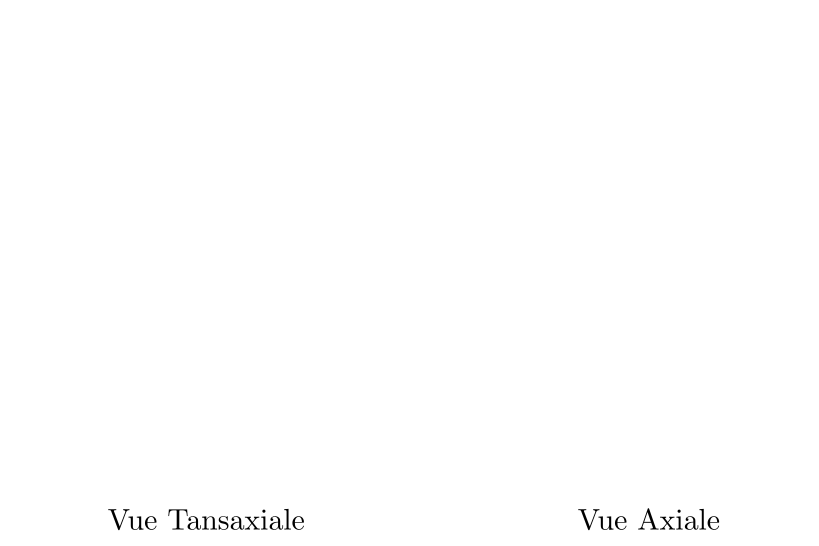
\includegraphics[width=12cm]{images/recalageLOR}
	\end{center}
	\caption[Illustration du recalage des lignes de réponse dans l'espace du détecteur]{Illustration du recalage des lignes de réponse dans l'espace du détecteur : $P_A$ et $P_B$ représentent les positions des détections, $P_{A'}$ et $P_{B'}$ les positions des points corrigés et $Q_A$ et $Q_B$ les détections correspondantes } 
	\label{fig:recalageLOR}
\end{figure}

\begin{figure}[h!]
	\begin{center}
		\includegraphics[width=6cm]{images/bloomfield2003design} \includegraphics[width=3cm]{images/livieratos2005rigid}
	\end{center}
	\caption[Résultats de l'algorithme de recalage des LDR sur des images de patients]{Résultats de l'algorithme de recalage des LDR sur des images de patients utilisant le radio-traceur [$^{11}$C]raclopride. (a) montre une image non corrigée du mouvement et (b) une image corrigée. On peut noter que les structures internes du cerveau sont beaucoup mieux définies. (c) représente une coupe du c\oe{}ur petit axe non corrigée (en haut) et corrigée (en bas). On peut voir une amélioration de la définition de l'image.} 
	\label{fig:ameliorationLOR}
\end{figure}
 

En effet,~\cite{lamare2007respiratory} réalise une estimation du mouvement, en recalant les images TDM de chaque instant du cycle sur l'image de référence à l'aide d'une transformation affine par maximisation de l'information mutuelle normalisée. Les données sont des simulations réalisées à partir du logiciel GATE~\cite{jan2004gate} et du fanôme NCAT. Des lésions de 7, 11, 15 et 21mm de diamètre ont été placées dans le poumon, avec un contraste de 8. Le champ de mouvement est calculé séparément pour le poumon, le coeur et trois organes sous le diaphragme (foie, estomac, rate).

Ces résultats ont été améliorés par l'utilisation de la technique suivante qui permettait la prise en compte d'un mouvement élastique. Les performances comparées des deux méthodes sont présentées dans la section suivante.

\section{Correction pendant la reconstruction}
\label{lab:CorrpendantRecon}
Plusieurs auteurs ont présenté des méthodes permettant de réaliser la correction de mouvement pendant la reconstruction. Qiao et al.~\cite{qiao2006motion} et Lamare et al.~\cite{lamare2007list} ont proposé une méthode de correction du mouvement respiratoire basé sur une modification de la matrice de sensibilité lors de la reconstruction pour prendre en compte le mouvement. Tous les deux utilisent un champ de mouvement élastique estimé en utilisant un champ interpolé par B-splines.

L'algorithme original utilisé est basé sur OPL-EM~\cite{reader2002one} qui organise les données en ``sous-ensemble'' de la même manière que OS-EM~\cite{hudson1994accelerated} mais en utilisant les informations séquentielles présentées en~\ref{lab:modeliste}. Le principe de la reconstruction avec correction du mouvement respiratoire est décrit par la formule suivante :

\label{lab:corrMatSyst}
\begin{equation}
 f^{k+1}=\frac{f^k}{S} \sum_{t=1}^{N} P_t^T \frac{1}{P_t f^k} 
\label{lab:OPLLamara}
\end{equation}

$f^k$ est l'image à l'itération $k$,

$T$ est l'opérateur de transposition

$P_t$ représente la matrice système à l'instant t. Chaque élément $p_{ij}^t$ de cette matrice indique la probabilité de détecter à la ligne de réponse $i$ un évènement généré au voxel $j$ au temps $t$. Cette équation est basée sur l'algorithme OPL-EM présenté en~\ref{lab:OPLEM}. Les informations du champ de mouvement sont contenues dans la matrice $P_t$. $P_t f$ correspond à la projection de l'image $f$ à l'instant $t$.  

$N$ correspond au nombre d'instants temporels considérés.

$S$ est la matrice de sensibilité :

\begin{equation}
 S=\frac{1}{N} \sum_{t=1}^{N} P_t^T M A_t 
\end{equation}

 $A_t$ est la matrice permettant de corriger les effets de l'atténuation au temps $t$ et $M$ est la matrice de normalisation qui compense l'inhomogénéité spatiale de la sensibilité. $A_t$ est estimée à partir des cartes d'atténuation de chaque instant $t$.

L'étude~\cite{lamare2007list} a été réalisée sur des données simulées semblables à celles de l'étude précédente. Il sagit de simulations réalisées à l'aide du logiciel GATE, d'un cycle respiratoire du modèle NCAT, constitué de 8 instants temporels ainsi qu'une acquisition statique de référence de statistique équivalente à la somme des 8 acquisitions précédentes. Des lésions de 7, 11, 15 et 21mm de diamètre et d'activité 8 fois plus importante que le fond ont été insérées dans le poumon.
 
Dans la publication, deux variantes de la technique de correction du mouvement respiratoire sont comparées avec la correction par synchronisation respiratoire avec recalage présentée précédemment ainsi que la correction pré-reconstruction. Les variantes correspondent à des différences d'interpolation du champ de mouvement dans la matrice système. Les résultats présentés montrent un clair avantage pour la correction pendant la reconstruction, avec des performances couramment améliorées d'un facteur 2. 

Par exemple, il utilise le PRD sur la métrique contraste (équation~\ref{eq:percentAmelioraiton}) pour une lésion de 7mm présente dans la partie haute du poumon est de 28\% pour les images non corrigées, contre 4.4\% pour les images corrigées par la méthode de correction pré-reconstruction et de 1.2\% pour la méthode de reconstruction pendant la reconstruction. De la même manière, pour des lésions de 7mm présentes dans le bas du poumon, les images non corrigées montrent une différence relative de contraste de 32\%, contre 2.63\% pour la correction pré-reconstruction et 1.66\% pour la correction pendant la reconstruction.


\begin{equation}
 \label{eq:percentAmelioraiton}
 \% Am\acute{e}lioration = \left| \frac{Contraste~sur~image~\acute{E}valu\acute{e}e~-Contraste~sur~R\acute{e}f\acute{e}rence}{Contraste~sur~R\acute{e}f\acute{e}rence} \right|
\end{equation}

La figure~\ref{fig:lamare2007} montre un profil de l'interface poumon/foie avec une tumeur pour les différentes techniques de correction. On voit clairement que l'image non corrigée montre un retard dû au flou de mouvement. Ce retard est partiellement corrigé par la correction de mouvement pré-reconstruction, mais le profil de courbe de la méthode de correction du mouvement pendant la reconstruction est celui qui s'approche le plus de la référence.


\begin{figure}[h!]
	\begin{center}
		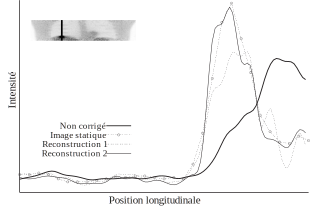
\includegraphics[width=12cm]{images/lamare2007list.pdf}
	\end{center}
	\caption[comparaison des performances des différentes techniques de correction du mouvement sur un profil d'image TEP]{comparaison des performances des différentes techniques de correction du mouvement sur un profil d'image TEP contenant une tumeur placée au niveau du diaphragme. La référence est l'image statique, ``Reconstruction 1'' correspond à la correction pré-reconstruction, et ``Reconstruction 2'' correspond à la correction pendant la reconstruction.} 
	\label{fig:lamare2007}
\end{figure}


\begin{figure}[h!]
	\begin{center}
			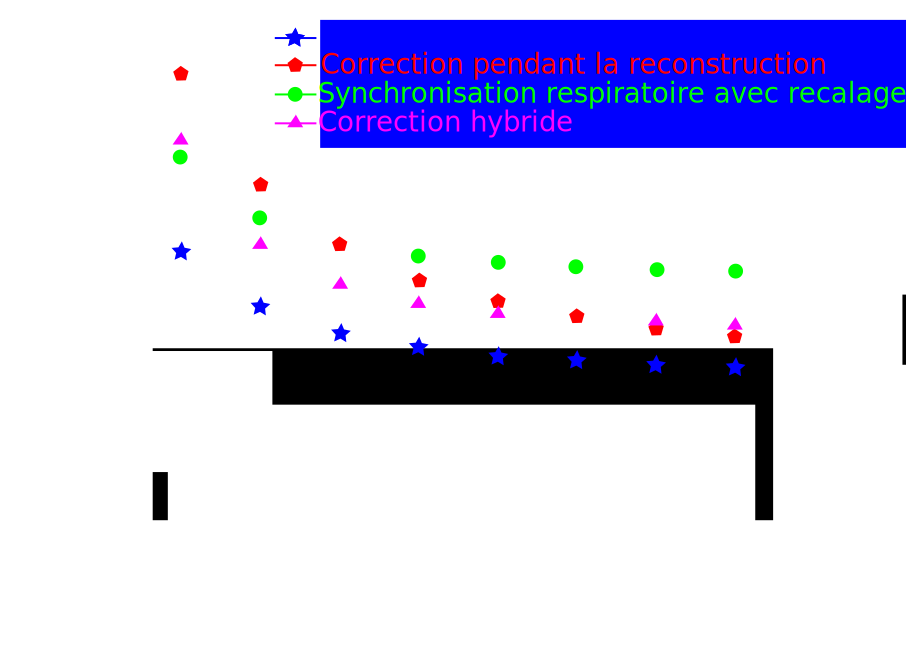
\includegraphics[width=10cm]{images/apportCHO}
	\end{center}
	\caption[Index de CHO pour différentes techniques de correction du mouvement respiratoire en fonction du nombre d'itérations de la reconstruction]{Index de CHO pour différents techniques de correction du mouvement respiratoire en fonction du nombre d'itérations de l'algorithme de reconstruction. Plus l'indice est important meilleure est la détectabilité. La méthode utilisant la correction post-reconstruction est comparée avec une méthode hybride présentée dans le document en~\ref{lab:evolGating}.} 
	\label{fig:apportCHO}
\end{figure}


 La publication~\cite{Thielemans2006Lesion} présente un système hybride de synchronisation respiratoire avec recalage et de correction de mouvement pendant la reconstruction. Ce système a été développé pour pouvoir isoler l'effet de la sommation des images recalées sur le résultat. Pour cela, les données de chaque instant temporel sont corrigées et reconstruites séparément à l'aide de la formule~\ref{lab:OPLLamara}. Les N images sont ensuite directement sommées pour obtenir l'image corrigée. La publication montre que cette technique hybride améliore de manière sensible la détection par rapport aux images non corrigées mais reste inférieure aux deux autres techniques mentionnées pour la mesure de détectabilité, comme présenté dans la figure~\ref{fig:apportCHO}
\label{lab:evolGating}

\section{Déconvolution de l'image}

Cette technique décrite dans~\cite{naqa2006deblurring} utilise une connaissance du mouvement respiratoire acquise à partir d'une image TDM 4D pour déduire un filtrage appelé TLP (\textit{Tumor Location Probability}) qui correspond à la dégradation dû au mouvement respiratoire. Un exemple de filtre est représenté sous forme 3D dans la figure~\ref{fig:formeTLP}.

\begin{figure}[h!]
	\begin{center}
		\includegraphics[width=10cm]{images/formeTLP}
	\end{center}
	\caption[Exemple de filtres TLP pour la correction par déconvolution]{Exemple de filtres TLP calculé dans l'article~\cite{naqa2006deblurring} pour la correction par déconvolution, rendu en 3D après tesselation,lissage et normalisation. Il représente la probabilité de présence du centre de la lésion.} 
	\label{fig:formeTLP}
\end{figure}



L'image est déconvoluée pixel par pixel pour corriger les effets du mouvement respiratoire. Cette méthode a été évaluée sur un fantôme physique et des patients réels à l'aide d'un grand nombre de critères provenant pour partie de la TEP (sous-estimation de l'activité de la tumeur, exemples d'images), et pour partie du domaine de la déconvolution (entropie, ``rugosité'').

Les résultats présentés sur la figure~\ref{fig:performanceDeconvolution} montrent une nette amélioration des performances sur des fantômes, pour un déplacement axial simple de 20 mm. L'activité des lésions de fort diamètre ($>$ 20 mm) est correctement récupérée quelque soit l'algorithme utilisé, mais il n'a pratiquement pas d'effets sur les lésions de 1 cm de diamètre.

Ce type de méthode est peu présent dans la littérature par rapport aux autres présentés précédemment. 

\begin{figure}[h!]
	\begin{center}
		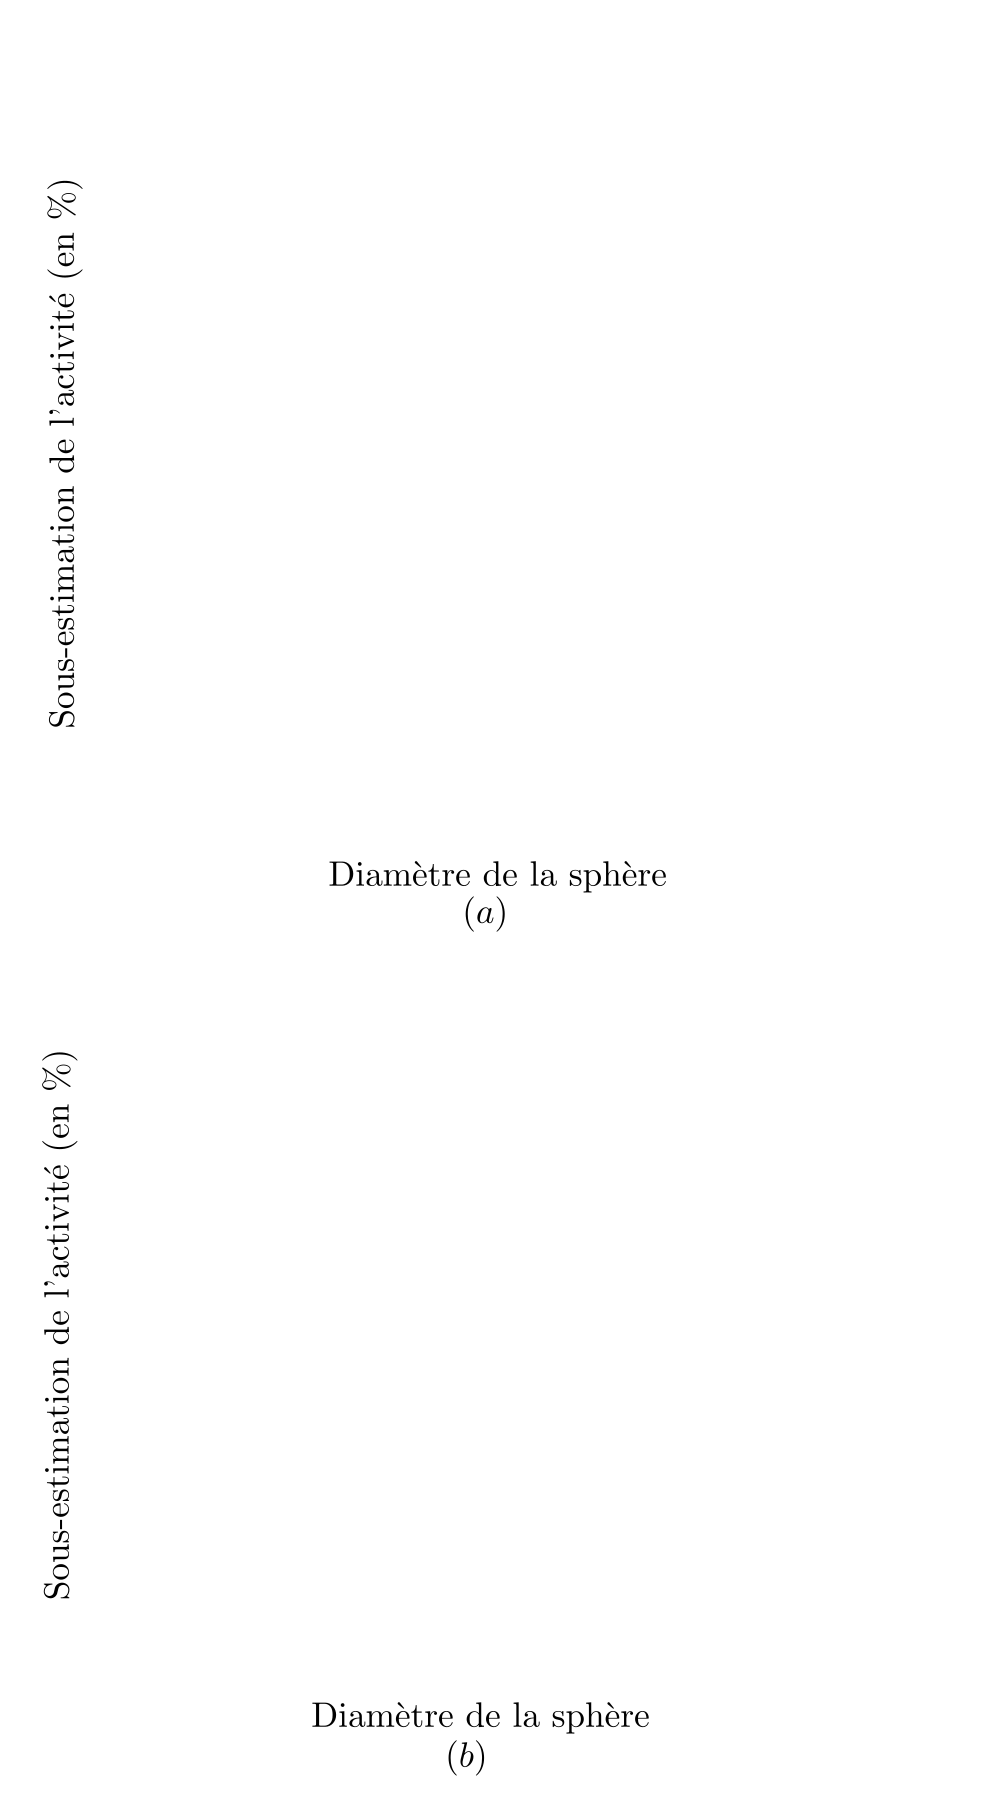
\includegraphics[width=10cm]{images/performanceDeconvolution}
	\end{center}
	\caption[Comparaison de l'erreur de sous-estimation de l'activité des lésions]{Comparaison de l'erreur de sous-estimation de l'activité des lésions en fonction de l'algorithme de déconvolution utilisé sur des fantômes. En a) la lésion a une activité moyenne, tandis qu'en b) l'activité de la lésion est faible par rapport au fond. Le déplacement de la lésion est le même dans les deux cas (2cm)} 
	\label{fig:performanceDeconvolution}
\end{figure}


Un autre article utilisant aussi des algorithmes de déconvolution a été présenté par Wiemker~\cite{wiemker2008combined}. Cependant il ne cherche pas à corriger le mouvement respiratoire sur l'ensemble de l'image mais principalement à améliorer la mesure du SUV sur une lésion. Pour cela, il réalise une estimation de la fonction d'étalement du point (FEP) de l'imageur TEP au niveau de la lésion à l'aide d'un contourage de la lésion réalisé préalablement sur une image TDM. L'estimation de la FEP permet de prendre en compte à la fois les effets du mouvement respiratoire et ceux de la FEP intrinsèque à l'imageur TEP. 

Cependant, cette technique est inapplicable dans notre cas car les lésions doivent être de taille suffisamment importantes et homogènes pour pouvoir les délimiter de manière fiable sur les images TDM.


\part{Evaluation des performances de détection}
	\chapter{Performance des outils de détection}
\label{lab:chapCAD}
	\section{Généralités}

En oncologie, la détection des sites tumoraux est une étape capitale dans la prise en charge des patients. 
Dans cette partie, je vais détailler les techniques qui permettent de comparer les performances de plusieurs observateurs (médecins ou algorithmes) face aux mêmes images, ou alors du même observateur face à plusieurs types d'images différentes.

Pour cette section, le problème va être simplifié au cas où un observateur doit classer un signal en ``Sain'' (normal, HO) ou ``Pathologique'' (anormal, H1). 

Les performances d'un classifieur sont indiquées par la matrice de confusion (table~\ref{tab:confusion}), qui recense les signaux correctement et incorrectement classés 

\begin{table}[h]
	\label{tab:confusion}
	\begin{tabular}{cc c|c|}
		& & \multicolumn{2}{c}{Classe estimée} \\
		\cline{3-4}	
		& & \multicolumn{1}{|c|}{Sain} & Pathologique \\ 
		\cline{2-4}
		\multicolumn{1}{c|}{\multirow{2}{*}{Classe réelle}} & \multicolumn{1}{|c|}{Sain} & VN (\emph{Vrai Négatif}) & FP (\emph{Faux Positif})\\
		\cline{2-4}
		\multicolumn{1}{c|}{} & \multicolumn{1}{|c|}{Pathologique} & FN (\emph{Faux Négatif}) & VP (\emph{Vrai Positif})\\
		\cline{2-4}
	\end{tabular}
	\caption[Matrice de confusion]{Matrice de confusion : donne une vue
d'ensemble des performances du classifieur. Elle indique le résultat de la
classification de signaux connus.}
\end{table}

On utilise habituellement deux grandeurs pour mesurer les performances d'un classifieur :

La \emph{sensibilité} (voir l'équation~\ref{eq:sensib}) correspond à la proportion d'images correctement évaluées pathologiques par l'observateur par rapport au nombre total d'images réellement pathologiques. Elle donne une information sur la capacité du classifieur à détecter les cas pathologiques.
\label{lab:pressensib}
\begin{equation}
	\label{eq:sensib}
	Sensibilit\acute{e} = \frac{VP}{VP + FN}
\end{equation}

La \emph{spécificité} (voir équation~\ref{eq:specif}) représente le même type de grandeur, mais cette-fois ci appliquée aux cas non pathologiques : elle correspond à la capacité du classifieur à donner un résultat négatif lorsque l'image est non pathologique.

\begin{equation}
	\label{eq:specif}
	Sp\acute{e}cificit\acute{e} = \frac{VN}{VN + FP}
\end{equation}

Ces deux grandeurs sont complémentaires mais ne permettent pas à elle seules de comparer des classifieurs. En effet, un  utilisateur va souvent donner des notes, qui vont indiquer son niveau de confiance sur la présence de la pathologie (à ne pas confondre avec des notations sur la gravité des lésions, comme les techniques de gradation de~\cite{genestie1998comparison}).

Les techniques de comparaison de systèmes de décision comme l'analyse ROC (Receiver-Operating Curve) permettent de prendre en compte ces incertitudes. Elles proviennent à l'origine du domaine des télécommunications pendant la seconde guerre mondiale, où il fallait une métrique permettant de tester les performances des systèmes RADAR~\cite{zou2007receiver} pour la détection des avions ennemis. Les courbes ROC servent donc à évaluer la capacité d'un ou plusieurs ``observateurs'' à discriminer des signaux entre deux classes ``normal'' et ``anormal''. Les informations de sensibilité et de spécificité se limitent à comparer les performances pour un niveau de confiance donné.

\subsection{Définition d'un Vrai positif / Faux positif}

En général, les systèmes CAD génèrent des cartes paramétriques, sur lesquels les voxels ou des groupements de voxels reçoivent une valeur correspondant à leur classe. 

Afin de déterminer si l'élément (voxel ou groupement de voxels) noté ``anormal'' fait effectivement partie d'une lésion, sa  position est généralement comparée à celle des lésions de la vérité terrain. Une distance d'acceptation est utilisée pour prendre en compte une éventuelle imprécision du système CAD. Par exemple, l'auteur de~\cite{paik2004surface} considère que l'élément est un vrai positif si il est contenu dans la tumeur de la vérité terrain.

Cependant, il existe plusieurs stratégies pour compter les FP :
\begin{itemize}
 \item Par voxel ou groupe de voxel (3D)
 \item Par coupe (2D)
\end{itemize}

Ces deux techniques vont très fortement influer sur le nombre de faux positifs pour le même système CAD. En effet, dans le cas où le comptage des FP est réalisé sur l'ensemble de l'image, chaque groupement ou voxel ne correspondant pas à une lésion est noté FP. L'auteur de~\cite{paik2004surface} indique par exemple 165 faux positifs par images TDM pour une sensibilité de 100\%. De même,~\cite{zhao2003automatic} montre une sensibilité de 94\% avec 906 faux positifs par image TDM pour la détection du cancer du poumon. Ces résultats montrent des nombre de faux positifs très importants, mais ne peuvent pas être comparés avec ceux utilisant un chiffrage des FP par coupe. En effet, dans ce cas, ``FP'' correspond au nombre de coupes contenant au moins un élément n'étant pas une tumeur. Le nombre de faux positifs est donc borné par le nombre de coupes, et ne fait pas de différences entre des coupes contenant un grand nombre de lésions et celles n'en contenant qu'une. 

\textbf{Dans le reste du document, nous considèrerons le premier système de comptage des Faux positifs : tout élément du volume à observer n'étant pas en contact avec une tumeur sera compté comme un faux positif.}


	\section{Méthodologie ROC - Receiver-Operating Curve}

Les courbes ROC~\cite{swets1982evaluation,metz1986roc} sont des courbes indiquant la spécificité et la sensibilité de l'observateur (humain ou numérique) pour différents niveaux de certitude. Elles fournissent une mesure objective des performances d'un observateur dans une tâche de discrimination entre deux classes. 

Elles peuvent être utilisées pour comparer les performances relatives de différents observateurs ou pour déterminer leurs paramètres optimaux. L’évaluation d'un observateur par la méthode ROC nécessite la création d'un jeu de données labellisées en deux classes : Normale (H0) et Pathologiques (H1). L'observateur va se voir présenter l'ensemble des images et devra les noter individuellement selon un barème défini à l'avance (par exemple 0: pas du tout pathologique, 1: potentiellement pathologique, 2:équivoque, 3: potentiellement pathologique, 4: définitivement pathologique). Par convention, plus la note (notée $\lambda$) sera élevée, plus l'observateur va considérer qu'il est en présence d'un cas pathologique. A l'inverse, une note basse va indiquer un cas présumé sain. 


\begin{figure}[h]
	\begin{center}
	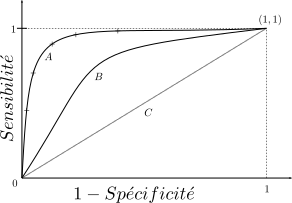
\includegraphics[width=10cm]{images/illustrationROC}
%	\vspace{-0.5cm} % Ugly Moche Hideux
	\end{center}
	\caption[Exemple de courbe ROC]{Exemple de courbe ROC. La courbe $A$ représente le résultat d'une évaluation ROC avec un barème à 6 niveaux. Pour chaque note du barème, le point correspondant est affiché en reportant la spécificité et la sensibilité (représentés par les croix). La courbe $B$ représente une autre évaluation, avec des performances inférieures : Pour chaque niveau de ``1-Spécificité'', la sensibilité de la courbe $B$ est inférieure à celle de la courbe $A$. Le courbe $C$ représente le d'un classifieur qui donne ses réponses de manière aléatoire.}
	\label{fig:illustrationROC}
\end{figure}

L'observateur peut être un humain ou un algorithme, et les notes peuvent être discrètes ou continues. 

Le tracé de la courbe ROC se fait en reportant la sensibilité et la valeur "1-spécificité" du classifieur pour différents seuils de décision. Par construction, la courbe va commencer au point $(0,0)$ (tous les points sont diagnostiqués négatifs) et se terminer au point de coordonnée $(1,1)$ (tous les points sont diagnostiqués positifs). Deux exemples de courbes ROC sont présentés sur la figure~\ref{fig:illustrationROC}.


Pour analyser les courbes ROC, on considère que les distributions de probabilité des notes des cas H0 et H1 suivent une loi gaussienne (voir figure~\ref{fig:loiROC}). Ce modèle de décision suppose que l'ensemble des valeurs de $\lambda$ évaluées sur des cas H0 (sain) suit une distribution de probabilité $P(\lambda_0, \sigma_0)$ de valeur moyenne $\lambda_0$ et d'écart-type $\sigma_0$. De même, les valeurs de $\lambda$ évaluées sur des cas H1 (pathologiques), suivent une distribution de probabilité $P(\lambda_1, \sigma_1)$. Le mécanisme de décision se base sur le choix d'une valeur de seuil $\lambda_s$ au-delà de laquelle les observations sont considérées comme pathologiques.

Ce seuil permet de modifier de manière dynamique la répartition des observations dans la matrice de confusion.  Cela permet d'enrichir la comparaison des observateurs par rapport au couple (sensibilité/spécificité) seul.

Selon cette hypothèse gaussienne, on peut montrer que la distance $d$, appelée indice de détectabilité, correspond à l'aire sous la courbe ROC :


\begin{equation}
 d= \frac{d_1 - d_0}{\sqrt{\sigma_1 + \sigma_0}}
\end{equation}

\begin{figure}[h]
	\begin{center}
	\includegraphics[width=10cm]{images/loiROC}
	\vspace{-0.5cm} % Ugly Moche Hideux
	\end{center}
	\caption[Modèle de la distribution de probabilité de la variable de décision]{Modèle de la distribution de probabilité de la variable de décision dans pour les populations H0 ($P(\lambda_0, \mu_0)$) et H1 ($P(\lambda_1, \mu_1)$) dans les études ROC. $\lambda_s$ représente le seuil à partir duquel une observation sera catégorisée H0 ou H1.}
	\label{fig:loiROC}
\end{figure}




Un ensemble d'indicateurs et de figures de mérite (FDM) permettent de comparer les performances de classifieurs à partir des courbes ROC. La FDM la plus simple consiste à choisir un niveau de spécificité (noté $\alpha$) et à comparer les sensibilités des différents classifieurs. L'avantage de ce système est qu'il permet de comparer les performances dans des conditions proches de la réalité, où l'on cherche à rester dans un taux de spécificité donné. Cependant, les résultats vont dépendre du paramètre $\alpha$. Une métrique plus globale est l'aire sous la courbe ROC. \'Etant donné que la courbe est nécessairement comprise dans un carré unitaire, la valeur de l'aire sera comprise entre 0 (le classifieur donne systématiquement les mauvaises réponses), 0.5 (le classifieur donne des réponses aléatoires) et 1 (le classifieur donne toujours la bonne réponse)~\cite{nie2006integrating}.

Il est important, lors du calcul de la FDM, d'avoir une estimation de l'erreur. Il est possible de l'estimer en ajustant une courbe théorique (répondant à la loi théorique de la figure~\ref{fig:loiROC}). Plusieurs logiciels ont été développés pour estimer les paramètres, qui ont été comparés dans la publication~\cite{CarstenStephan03012003} (AccuROC, Analyse-It, CMDT, GraphROC, MedCalc, mROC, ROCKIT, and SPSS).

\label{lab:p-valeur}
Une grandeur souvent utilisée dans la littérature pour évaluer la pertinence d'un résultat est la \emph{p-valeur}. Elle représente la probabilité d'obtenir des différences entre deux courbes au moins aussi extrême que la différence observée (dans notre cas, les courbes ROC), en prenant en compte l'hypothèse selon laquelle le classifieur est aléatoire. Elle permet de vérifier si le test est statistiquement significatif.

Le problème de la méthodologie ROC est que l'observateur ne donne pas d'information de localisation de la pathologie dans l'image. On lui présente une image et il doit la noter sans indiquer la localisation de la zone suspecte. Dans notre cas, nous voulons comparer des classifieurs qui détectent les tumeurs dans l'image. Il faut non seulement savoir si des lésions sont présentes, mais aussi avoir leur nombre et leur localisation. Cela est proche du travail en routine clinique, qui consiste à évaluer l'étendue et le nombre des lésions pour déterminer l'efficacité d'un traitement par exemple. 

Pour éviter cette limitation, plusieurs extensions à la méthodologie ROC sont décrites dans la littérature : L-ROC, AF-ROC ou encore F-ROC. Les L-ROC sont décrites ci-après, tandis que les AF-ROC et F-ROC seront décrites dans la section suivante.

\subsection{Courbes ``Localization ROC'' (L-ROC)}

L'analyse L-ROC~\cite{farquhar1999roc} ajoute l'information de localisation lors de la décision. L'observateur doit indiquer sur l'image qu'il considère comme pathologique la localisation de la lésion la plus probable. Elle est considérée comme un vrai positif si la distance entre la localisation indiquée et la localisation réelle de la lésion est inférieure à une certaine distance.

Cependant, bien que cette technique prenne en compte l'information de localisation, elle ne permet pas de traiter de manière satisfaisante les cas de lésions multiples.


\section{Courbes Free ROC}	

Les courbes Free-ROC permettent de prendre en compte plus d'informations que les courbes vues précédemment car elles utilisent non seulement les informations de localisation, mais prennent aussi en compte le concept de faux positifs de manière plus approfondie, avec la possibilité d'avoir à la fois des faux positifs et des vrais positifs dans une même image.

\subsection{Courbes Free-ROC}
\label{lab:FROC}

Les courbes F-ROC~\cite{bunch1978free} sont une généralisation des courbes ROC aux cas où l'on évalue la capacité de l'observateur à détecter un ensemble de lésions dans une série d'images. Chaque image pouvant contenir un nombre indéfini de lésions. L'observateur va donc devoir pointer sur l'image l'ensemble des sites suspects et y associer une note.

Dans ce cas, on ne peut pas utiliser le formalisme ROC car le terme de spécificité n'est pas directement calculable pour chaque niveau de confiance. On utilise à sa place le nombre moyen de faux positifs par image pour un seuil donné (voir figure~\ref{fig:courbeFROC}).

On utilise les termes de LL (Lésion localisée) et NL (Non-Lésion) en lieu et place des informations de vrai positifs et faux positifs sur les courbes ROC. De la même manière, la sensibilité et la spécificité sont respectivement FLL (Fraction de lésions correctement détectées et localisées) et NFM (Nombre de faux positifs moyens par image).


\begin{figure}[h]
	\begin{center}
	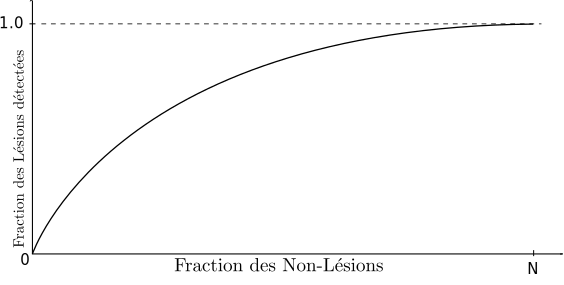
\includegraphics[width=15cm]{images/FROC}
	\end{center}
	\caption{Exemple de courbe Free ROC}
	\label{fig:courbeFROC}
\end{figure}

Les courbes F-ROC n'ayant pas de bornes sur l’axe des abscisses, il est impossible de comparer plusieurs courbes à partir de l'aire sous la courbe. Il reste cependant possible de comparer la sensibilité pour un nombre de faux positifs donnés, mais on retrouve les mêmes problèmes que pour l'analyse ROC : il faut choisir un paramètre.

\subsection{Courbes Alternative Free-ROC}

Les courbes A-FROC~\cite{chakraborty1990free} sont des extensions des courbes Free-ROC présentées précédemment mais qui ne prennent en compte que le faux positif de plus haut score par image, ce qui ne pénalise pas le cas où un observateur indique un grand nombre de fausses détections (NL). On se retrouve alors dans la situation de courbes bornées sur l'axe des abscisses, ce qui permet leur comparaison.

\subsection{Comparaison des courbes}
\label{lab:AFROC}
Plusieurs techniques ont été développées pour permettre de réaliser des comparaisons de courbes dérivées de la méthodologie F-ROC. De la même manière que pour les courbes ROC, il est possible de comparer les courbes F-ROC en fonction de la FLL pour un nombre de faux positifs donnés. Cependant, étant donné que les courbes F-ROC n'ont pas de fin déterminée, il n'est pas possible d'utiliser l'aire sous la courbe. 

JAFROC~\cite{chakraborty2004observer} (JAcknife Free Receiver Operating Curve) est un algorithme et un logiciel développé par Chakraborty et se base sur une FDM non liée directement à la courbe. Cette mesure de performance utilise un algorithme dérivé des études A-FROC, ce qui signifie qu'il n'utilise pas l'ensemble des informations disponibles dans les courbes F-ROC mais se borne à comparer les scores des faux positifs de plus forte note pour chaque image avec les notes des vrais positifs. La figure de mérite $\Theta_J$ proposée mesure la probabilité d'avoir un score de vrai positif supérieur à celui d'un faux positif (de n'importe quelle image).

Soit $\theta_J$ la valeur de la FDM, $N_T$ le nombre total d'images, indexées par $i$, $N_A$ le nombre total de cas pathologiques, indexées par $j$. $n_j$ est le nombre total de lésions dans le cas anormal $j$.

\begin{equation}
\label{eq:JAFROC1}
\begin{array}{l}
	\displaystyle \theta=\frac{1}{N_T N_A} \sum_{i=1}^{N_T} \sum_{j=1}^{N_A} \sum_{k=1}^{n_j} W_{jk} \psi(X_i, Y_{jk}) \\
	\\
	\displaystyle \psi(X,Y) = \left\{
		\begin{array}{lll}
			1.0 & \mbox{si} & Y > X \\
			0.5 & \mbox{si} & Y = X    \\
			0.0 & \mbox{si} & Y < X    \\
		\end{array}
	\right. \\
	\\
	\displaystyle \mbox{avec} \sum_{k=1}^{n_j} W_{jk} = 1 \\
\end{array}
\end{equation}

$X_i$ le score du plus haut faux positif de l'image $i$, $Y_{jk}$ est la note de la lésion k de l'image j. Si une lésion n'a pas été détectée, alors sa note sera par défaut de "0".

Les poids $W_{jk}$ correspondent à l'importance relative de détecter la lésion $k$ dans l'image $j$ pour le diagnostic. Pour chaque image, la somme des poids doit être égale à 1.

Une seconde version de JAFROC existe avec une puissance statistique plus importante, mais elle nécessite de disposer d'un grand nombre de cas non pathologiques. La formule est la même que la précédente (équation~\ref{eq:JAFROC1}). La seule différence est que la première sommation se fait sur l'ensemble des cas non pathologiques $N_N$ (équation~\ref{eq:JAFROC2}) au lieu de l'ensemble des cas $N_T$.

\begin{equation}
\label{eq:JAFROC2}
\theta=\frac{1}{N_T N_A} \sum_{i=1}^{N_N} \sum_{j=1}^{N_A} \sum_{k=1}^{n_j} W_{jk} \psi(X_i, Y_{jk})
\end{equation}


\chapter{Systèmes de détection}

	\section{Les CAD en TEP}

Les systèmes CAD (Computer-Aided-Detection) sont des algorithmes permettant d'assister le praticien dans la détection des lésions ou le classement des images médicales. Dans le cadre de l'imagerie TEP oncologique, le besoin principal est celui du suivi thérapeutique, pour lequel, il est important de détecter d'éventuelles lésions résiduelles. Pour cela, il faut que le système CAD soit particulièrement adapté à la recherche de petites lésions de faible contraste qui pourraient échapper au médecin. Cependant, le diagnostic, qui consiste à évaluer la dangerosité des lésions, et leur caractère pathologique est une tâche plus complexe qui relève plus des systèmes d'aide au diagnostic, qui ne seront pas traités ici.

Le développement des systèmes CAD a débuté dans les années 1980~\cite{chan1987image}, notamment pour détecter les micro calcifications en mammographie. Bien qu'il existe plusieurs systèmes CAD commerciaux pour l'imagerie TDM (xLNA pour philips par exemple), aucun CAD commercial pour la TEP n'existe à notre connaissance.

Cependant, plusieurs CAD sur des images TEP ont été décrits dans des travaux académiques, tels que~\cite{guan2006automatic}, qui recherche des anomalies dans le corps entier. Cependant, ils ne donnent pas de mesures de performances quantitatives. La publication de~\cite{Kanakatte2008pulmonary} utilise des systèmes de classification supervisés (K plus proches voisins et SVM décrits en~\ref{lab:SVM}). Un seuillage est réalisé, puis les candidats sont classés en utilisant des caractéristiques fréquentielles et les moments statistiques. 

<Ajouter CAD présentés dans le papier de TNS>

Cependant les systèmes de classifications existants se concentrent en général sur la délimitation de lésions de fort contraste, ce qui ne correspond pas à notre problématique de détection. 

	\section{Méthodes de classification}

Dans cette section je vais décrire les deux principales classes de techniques de classification : supervisée et non supervisée.

		\subsection{Méthodes non supervisées}

 Dans le système de classification non supervisé, le classifieur reçoit directement l'ensemble des données à traiter, sans informations supplémentaires. Il devra de lui-même les classer par similitude en groupes. On utilise ce type de classifieur si on ne connaît pas a priori les classes, comme présenté dans la figure~\ref{fig:fonctionnementClassifNonSup}. Le nombre de classes peut être un des paramètres d'entréen notamment pour les k-moyennes, ou être déterminé de manière automatique.


La classification non supervisée repose sur une méthode statistique utilisant une fonction de proximité. Toutes les observations d'une même classe devront être proches au sens de cette fonction. Le partitionnement idéal est obtenu lorsque la covariance intraclasse est minimisée, ce qui implique que les classe sont le plus homogène possible, et que la distance entre les classes est maximisée, pour que les classes soient le plus différencié possible.

Plusieurs algorithmes sont décrits dans la littérature pour réaliser des classifications non supervisées :

\begin{description}
 \item[K-moyennes : ] c'est un algorithme itératif qui associe à chaque point la classe dont le barycentre est le plus proche, puis remet à jour le centre des classes à la prochaine itération~\cite{herwig1999large}.
 \item[Cartes auto-adaptatives : ] Cet algorithme utilise des techniques dérivées des graphes pour partitionner les données~\cite{kohonen1982self}.
 \item[Regroupement ascendant hiérarchique : ] Cet algorithme utilise une mesure de dissimilarité pour regrouper les observations. A la première itération, chaque observation dispose de sa propre classe. A chaque itération suivante, les deux classes contenant les observations les plus proches vont être regroupées, jusqu'à obtenir la classification finale~\cite{ward1963hierarchical}.
\end{description}


\begin{figure}[h]
	\begin{center}
	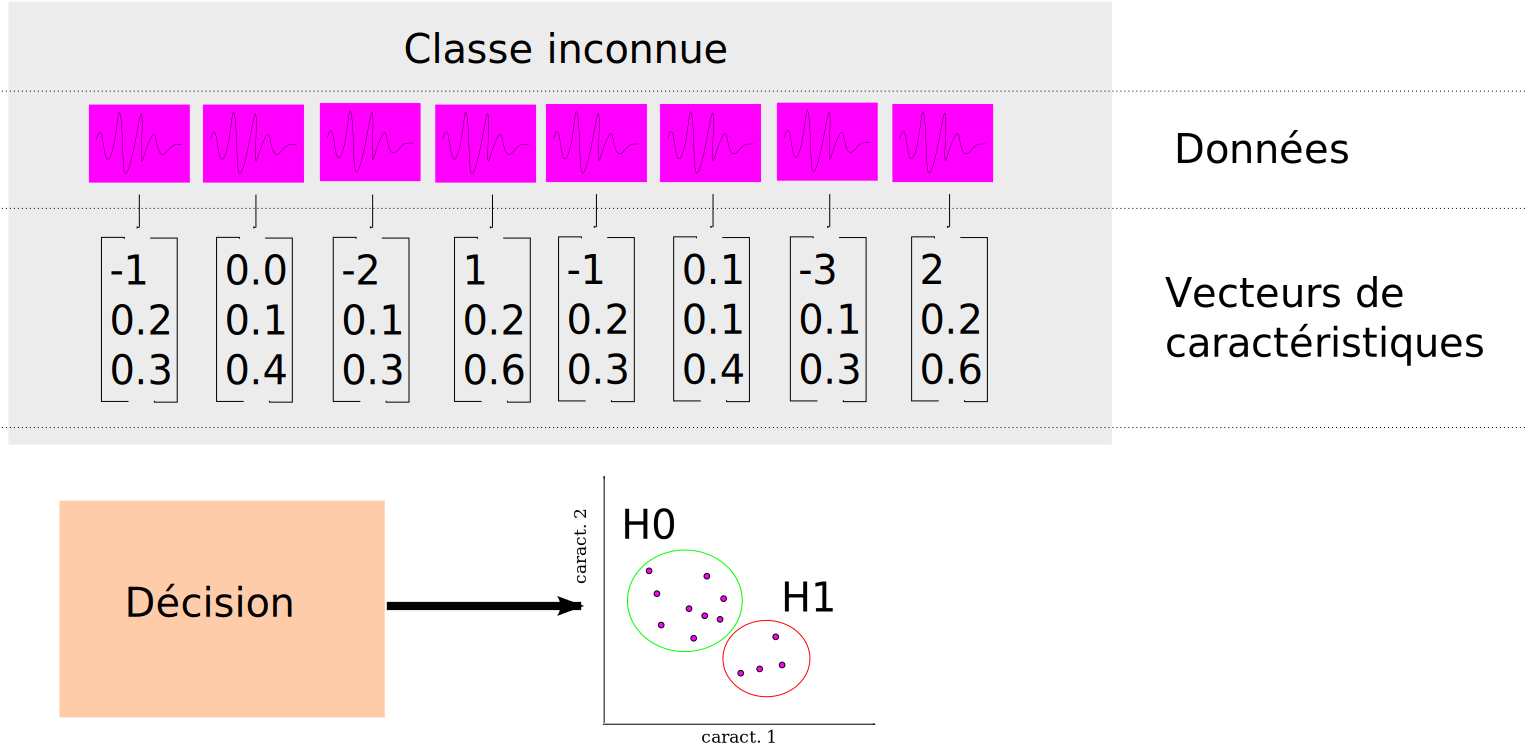
\includegraphics[width=15cm]{images/fonctionnementClassifNonSup}
	\end{center}
	\caption[Fonctionnement d'un classifieur non supervisé]{Fonctionnement d'un classifieur non supervisé : Les données brutes sont envoyées au classifieur qui va les regrouper en classes en fonction de leur répartition dans l'espace des caractéristiques.}
	\label{fig:fonctionnementClassifNonSup}
\end{figure}


		\subsection{Méthodes supervisées}

La classification supervisée vise à étiqueter des observations à partir de connaissances acquises à priori.

Les classifieurs supervisés nécessitent une connaissance a priori des classes. On entraîne le classifieur en lui fournissant des \emph{exemples} de cas avec l'étiquette associée. A partir de cette base de données d'entraînement, le classifieur va générer un \emph{modèle} prédictif permettant de classer de futurs exemples non encore connus, comme présenté dans la figure~\ref{fig:fonctClassif}.

\begin{figure}[h]
	\begin{center}
	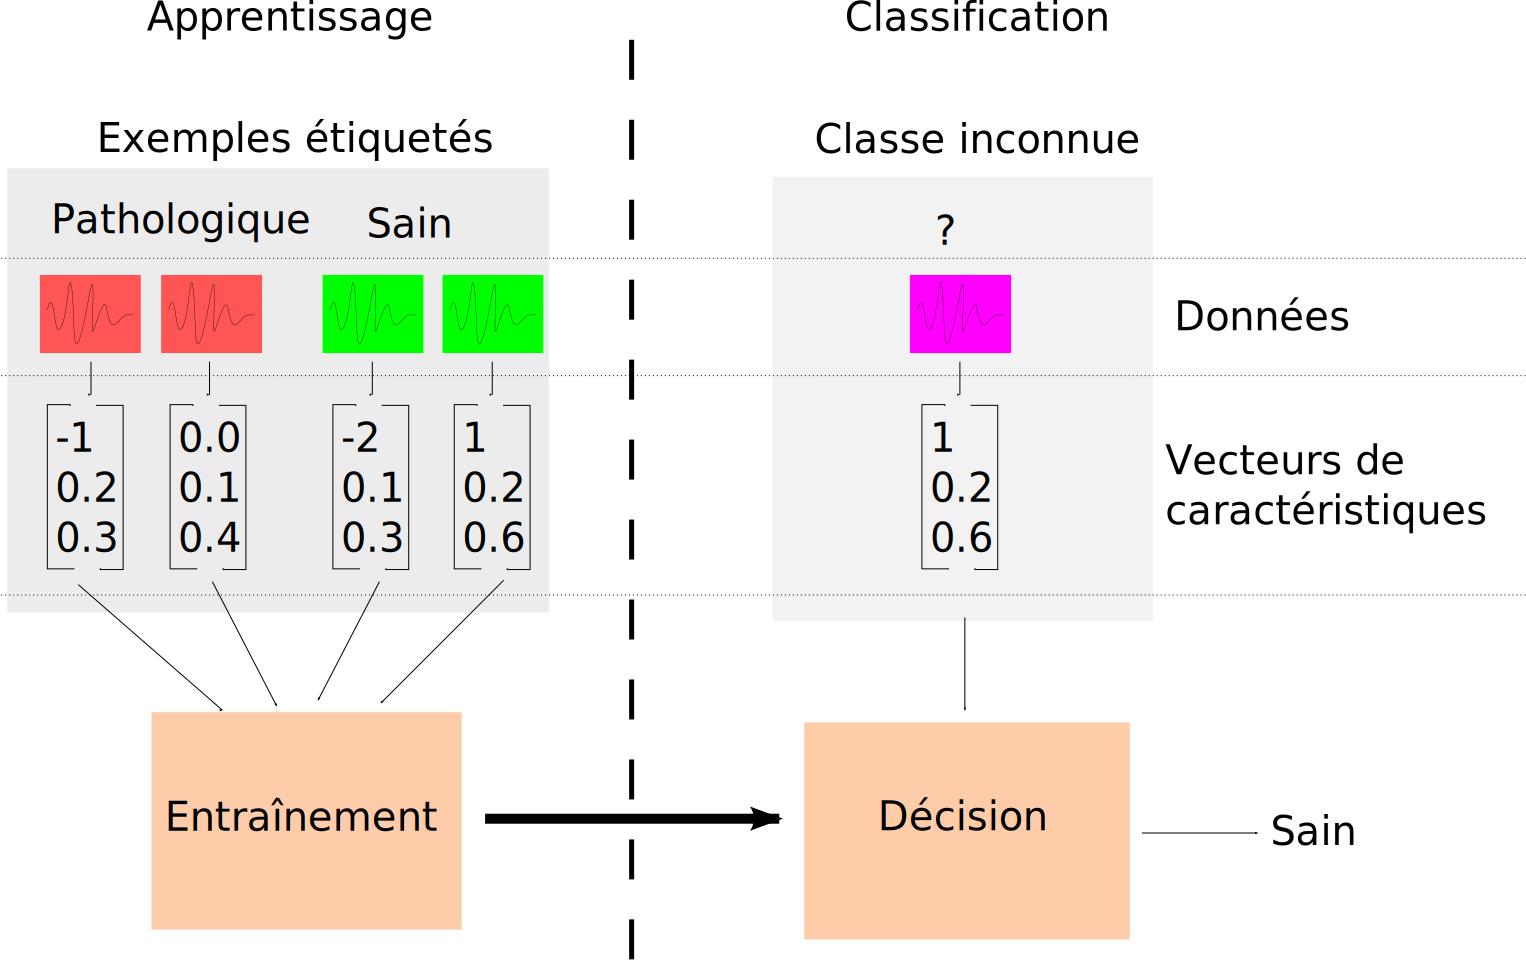
\includegraphics[width=15cm]{images/fonctionnementClassif}
	\end{center}
	\caption[Fonctionnement d'un classifieur supervisé]{Fonctionnement d'un classifieur supervisé : Les données d'apprentissage servent à entraîner le classifieur pour générer un modèle. Ce modèle permettra de rattacher des observations aux classes apprises.}
	\label{fig:fonctClassif}
\end{figure}


	\section{Machines à vecteur de support}

\label{lab:SVM}
La ``Machine à Vecteur de Support'', aussi appelée ``Séparateur à Vaste Marge'', ou ``Support Vector Machine'' en Anglais, est un classifieur qui comme son nom l'indique vise à maximiser la marge~\cite{boser1992training}, qui est la distance minimale entre les points des données et la surface séparatrice (voir figure~\ref{fig:SVM}).

\begin{figure}[h]
	\begin{center}
	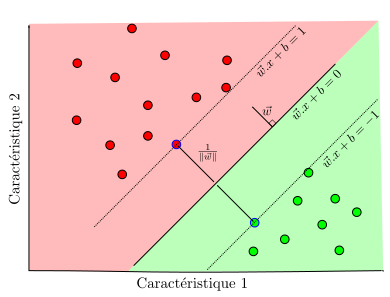
\includegraphics[width=12cm]{images/SVM}
	\end{center}
	\caption[Machine à Vecteur de Support]{Machine à Vecteur de Support : Les points vecteur de support (entourés de bleu) sont les seuls utilisés pour calculer la surface de séparation d'équation $w . x + b = 0$. Le vecteur $w$ est normal à la surface de séparation et permet de calculer la marge $\frac{1}{\Vert w \Vert}$.}
	\label{fig:SVM}
\end{figure}


Les SVM sont des classifieurs supervisés qui cherchent à maximiser la séparation entre chaque classe. L'idée sous-jacente aux SVM est de trouver l'hyperplan optimal de séparation, et non pas n'importe quel hyperplan qui permettrai de séparer correctement les données d'apprentissage (figure~\ref{fig:multiPlansSeparationSVM}). 


\begin{figure}[h]
	\label{fig:multiPlansSeparationSVM}
	\begin{center}
	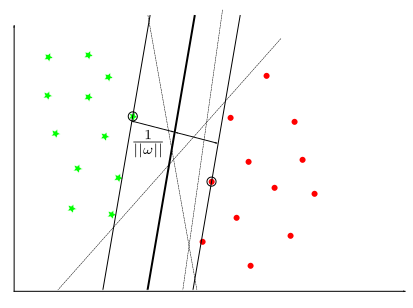
\includegraphics[width=15cm]{images/multiPlansSeparationSVM}
	\end{center}
	\caption[Illustration du principe d'optimisation de la marge sur le SVM]{Illustration du principe d'optimisation de la marge sur un cas à deux classes et deux caractéristiques : Il existe une infinité d'hyperplan qui séparent correctement les classes ``étoile vertes'' et ``ronds rouge'', représentés par les traits fins en pointillé. Cependant, il existe seulement une seule solution qui va maximiser la marge. Cette solution est représentée en trait plein, avec la marge $\frac{1}{||w||}$. Les points entourés en noir sont les points support utilisés pour contraindre l'hyperplan. }
\end{figure}


La définition de la marge et de l'hyperplan se fait à partir des vecteurs de support. Ils correspondent aux cas extrêmes des deux classes qui pourraient éventuellement poser des problèmes de classification.


Soit $\{(x_i, y_i) | x_i \in \mathbb{R}^p , y_i \in \{ -1, 1 \} \}$ un ensemble de points étiquetés correspondant à la base d'apprentissage. $x_i$ correspond au vecteur caractéristique, tandis que $y_i$ correspond à la classe du point.

Tout hyperplan dans l'espace des caractéristiques $\mathbb{R}^p$ peut être écrit $w . x - b = 0$, avec $w$ la normale à l'hyperplan et $\frac{b}{ ||w|| }$ le décalage de l'hyperplan par rapport à l'origine. 

La contrainte principale sur $w$ et $b$ est de classer correctement les données. Pour cela, les points vecteur de support devront respecter la contrainte $y_i ( w . x_i - b ) >= 1$. Par construction, les vecteurs de support correspondent aux points où l'égalité stricte est observée : $y_i ( w . x_i - b ) = 1$, comme indiqué sur la figure~\ref{fig:SVM}.

La seconde contrainte est la maximisation de la marge, qui correspond à  $\frac{2}{||w||}$, ce qui revient à minimiser $||w||$

La solution de ce problème d'optimisation est apportée par l'algorithme des multiplicateurs de Lagrange. 

Cependant, il peut arriver que les classes ne soient pas séparables. Ce problème est résolu par l'autorisation d'une erreur~\cite{cortes1995support} $\xi_i$  que l'on cherchera à minimiser : $( w . x_i - b ) >= 1 - \xi_i $. Cela engendre l'ajout d'un paramètre de classifieur noté $C$, qui sera utilisé dans le lagrangien pour pénaliser plus ou moins les erreurs.

Dans le cas où l'hyperplan de séparation ne pourrait pas être défini par une équation linéaire, des fonctions à noyaux sont utilisées pour projeter les points dans un espace de plus grande dimensions où le problème devient linéaire (voir figure~\ref{fig:kernelTrick}). Cependant, la transformation n'est jamais réalisée explicitement car en pratique, le changement de dimension est utilisé uniquement lors de la comparaison entre les points. On utilise donc des fonctions de comparaison modifiées, appelées noyaux. Le noyau le plus couramment utilisé est le RBF (fonctions à base radiale) qui a un espace d'arrivée de dimensions infinies :

\[ 
k(x_i,x_j)=e^{-\gamma||x_i-x_j||^2}  
\]

\begin{figure}[h]
	\begin{center}
	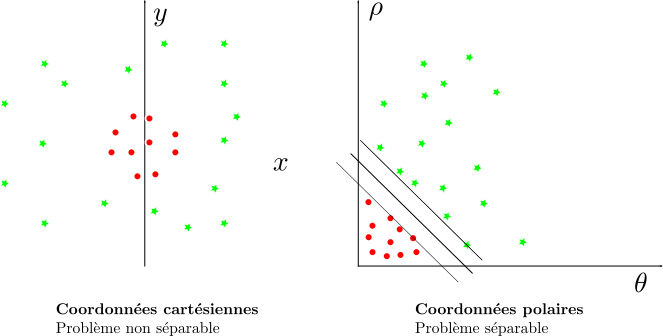
\includegraphics[width=15cm]{images/kernelTrick}
	\end{center}
	\caption[Changement de base pour les SVM]{Illustration du principe du changement de base : Des données non séparables dans le repère original peuvent devenir séparables en utilisant les noyaux. Dans ce cas, le passage des coordonnées cartésiennes aux coordonnées polaires permet de rendre le problème original linéairement séparable.}
	\label{fig:kernelTrick}
\end{figure}


Grâce à la maximisation de la marge, les SVM sont performants dans le cas où l'on ne dispose que de faibles quantités de données. D'autres algorithmes tels que les forêts aléatoires parviennent à obtenir des performances similaires~\cite{statnikov2008comprehensive}.

\subsection{Autres classifieurs supervisés}

De nombreux classifieurs supervisés ont été développés :

\label{lab:LDA}
Le classifieur LDA~\cite{fisher1936use} approxime les deux classes en supposant qu'elles ont une distribution gaussienne de covariance égale. Seule la moyenne de chaque distribution varie, et tout nouveau point est classé en fonction de sa distance à l'une ou l'autre des classes. Bien qu'il soit très rapide, ce classifieur ne fonctionne que dans le cas linéaire. Mais l'approximation gaussienne fonctionne donne des résultats suffisament bons dans de nombreux cas, ce qui explique son utilisation pour la détection des lésions en mammographie~\cite{baydush2007incorporation} ou en oncologie TDM~\cite{gurcan2002lung}.


Les réseaux de neurones~\cite{haykin1999neural} sont un classifieur non linéaire qui se base sur un fonctionnement simplifié des neurones du cerveau humain. il est constitué de neurones artificiels qui miment les réactions des neurones biologiques. Un neurone applique une fonction à la combinaison linéaire de ses stimuli d'entrée. Chaque élément du vecteur de caractéristique est entré dans un neurone, qui ira stimuler un ou plusieurs autres neurones. L'information se propage jusqu'à un neurone terminal qui donnera le résultat. Les réseaux de neurones sont très performants, mais souffrent de difficultés de mise en place à cause de leur grand nombre de paramètres et de temps d'apprentissage très importants.

Une forêt de décision est un classifieur relativement récent basé sur plusieurs arbres de décisions initialisés différemment~\cite{ho1998random}. Le résultat de ce classifieur est le mode des résultats de tous les arbres. La combinaison de plusieurs arbres différents permet d'améliorer la stabilité du classifieur, qui est un gros désavantage des arbres de décision pris indépendamment. Ce classifieur est très rapide et très performant

\section{Avantages et inconvénients des systèmes CAD}

Les systèmes CAD permettent de surmonter les inconvénients des observateur humain lors des évaluation de méthodes. Ils permettent de limiter la variabilité inter-observateurs en permettant de réaliser l'ensemble des détections avec un seul observateur, et garantissent que toutes les observations réalisées dans les mêmes conditions. Il est aussi possible de reproduire à l'identique les conditions d'évaluation pour traiter de nouvelles données.

Par contre, il n'y a aucune garantie que les systèmes CAD se comportent comme des observateurs humains. Pour cette raison, il est nécessaire de réaliser une validation du système CAD à l'aide d'observateur humain.


	\chapter{Choix méthodologiques}


La problématique de ce travail de thèse relève du domaine de l'évaluation en imagerie médicale. Cette discipline nécessite :

\begin{itemize}
 \item De bien définir la tâche.
 \item De choisir les bonnes métriques.
 \item De disposer d'une référence (ou vérité terrain).
\end{itemize}

Pour nous, la tâche diagnostique est d'améliorer la détection. Dans ce court chapitre, nous justifierons les choix méthodologiques que nous avons dû faire, d'une part pour la construction de la vérité terrain et d'autre part pour définir la méthode d'évaluation des performances de détection.

\section{Construction de la vérité terrain}

Le choix des types de données à utiliser pour une étude relevant du domaine de l'évaluation est important. Les différentes étapes de cette méthode d'évaluation sont présentées dans le chapitre 12. Pour notre problème, il est important de disposer de données TEP oncologiques dynamiques et synchronisées à la respiration contenant des lésions parfaitement annotées. La collection d’images cliniques annotées est un travail de longue haleine nécessitant le concours de différentes personnes, et principalement des cliniciens. 


Quelques bases de cas cliniques sont disponibles en imagerie TEP oncologiques. Celles-ci ne sont cependant pas distribuées à la communauté scientifique, sont rarement annotées et ne présentent pas forcément assez d’images de chaque classe. La littérature des CAD en imagerie TEP (section ~\ref{lab:CADTEP}) confirme ce manque de bases d’images cliniques distribuées car les auteurs utilisent généralement quelques cas fournis par les hôpitaux partenaires de leur étude. 

Une alternative à l’utilisation d’images cliniques repose sur la simulation d’examens. La quatrième partie de ce manuscrit s'attache à décrire la méthode utilisée pour créer notre jeu de données TEP 3D simulées avec la respiration, puis à décrire les caractéristiques de cette base de données.

Nous avons cherché à générer une base de données réaliste prenant en compte la variabilité rencontrée dans les acquisitions réelles. Pour cela, nous avons utilisé un modèle de patient déformable incorporant un modèle de respiration pour générer les images. Cela permet d'incorporer une variabilité importante dans les formes des organes patients de la base de données. Un mouvement respiratoire irrégulier a été utilisé pour générer les données, pour prendre en compte les imprécisions des systèmes d'acquisition du signal respiratoire. 


Les contrastes des lésions ont été calibrés pour obtenir des taux de détection par un observateur humain de 10\% à 90\%. Les activités des organes sont calculées à partir de zones d'intérêts extraites de 70 images TEP. La simulation a été réalisée avec le logiciel PET-SORTEO, utilisant des algorithmes Monte-Carlo accélérés. Nous avons simulé deux jeux de données : le premier correspond à une acquisition dynamique d'un patient respirant, avec 4 cycles respiratoires différents. Les cycles ont été coupés en 8 instants temporels simulés séparément pour représenter une acquisition synchronisée. Le second jeu de données correspond à une acquisition statique de même durée que le précédent (224 secondes), mais sans mouvement respiratoire. Il va être utilisé comme ``témoin'', correspondant à une hypothétique correction parfaite du mouvement respiratoire.

La quatrième partie de ce manuscrit s'attarde à décrire la méthode utilisée pour créer notre jeu de données TEP 3D simulées avec la respiration, puis à décrire les caractéristiques de cette base de données.

\section{Mesure des performances de détection}

Nous avons montré dans le chapitre 7 que les analyses ROC ou F-ROC sont les méthodes de référence pour évaluer les performances de détection. Ces études sont néanmoins lourdes à mettre en oeuvre lorsque l'on cherche à optimiser des paramètres et requièrent la participation active d'observateurs, souvent difficiles à mobiliser lorsque les tâches de lecture sont longues et répétitives.

Nous avons donc cherché à développer une stratégie qui permette de respecter les conditions de l'analyse F-ROC tout en s'affranchissant d'observateurs humains.

Le chapitre 8 a présenté le principe des systèmes d'aide à la détection, développés pour fournir une seconde lecture au médecin lors de son diagnostic. Nous avons proposé d'utiliser ces systèmes CAD comme observateurs numériques.

Les systèmes CAD permettent de surmonter les inconvénients des observateur humain lors des évaluations de méthodes. Ils permettent de limiter la variabilité inter-observateurs en permettant de réaliser l'ensemble des détections avec un seul observateur, et garantissent que toutes les observations sont réalisées dans les mêmes conditions. Il est aussi possible de reproduire à l'identique les conditions d'évaluation pour traiter de nouvelles données.

Nous avons développé une méthode d'évaluation des performances de correction basée sur l'utilisation d'un système de détection des lésions automatisé. Les performances de ce système de détection sur les lésions présentes dans les modèles vont définir la qualité et la pertinence de la correction. 

Nous utilisons un classifieur basé sur les Machines à Vecteurs de Support (SVM) utilisant les coefficients d'ondelettes non décimées comme caractéristiques fréquentielles. La classification est réalisée sur chaque voxel des images, puis une étape de réduction des faux positifs est appliquée, en agrégeant les voxels classés positifs, et en supprimant les agrégats de trop petite taille.

Les performances sont mesurées par l’analyse psychophysique des courbes free-receiver operating characteristics (FROC) que nous avons adaptée aux spécificités de l’imagerie TEP. L’évaluation des performances est réalisée sur deux méthodes prometteuses de correction du mouvement respiratoire, en les comparants avec les performances obtenues sur les images non corrigées ainsi que sur les images idéales sans mouvement respiratoire.


\part{Construction d'une base d'images TEP simulées respirante}
	\chapter{Simulations}

Simuler des images réalistes est un enjeu important en imagerie médicale. Le fait d'avoir accès à la vérité terrain, contrairement à la routine clinique, permet de valider des hypothèses de manière beaucoup plus fine. De plus, avec l'augmentation des performances de ordinateurs et l'accès à des centres de calculs, il devient possible de créer des bases de données de patients de plus en plus importantes et réalistes.

\todo{positionner par rapport à la TEP}

	\section{principe des simulations}

		\subsection{Simulations analytiques}

Les simulateurs analytiques ne simulent pas de manière réaliste le déplacement des particules mais  utilisent des approximations fortes pour résoudre les problèmes de manière analytique.

Dans le cas de l'imagerie TEP, la simulation analytique revient à réaliser des projections du volume TEP dans l'espace du sinogramme. Ce sinogramme est ensuite bruité et modifié pour prendre en compte les effets des coïncidences aléatoires, ou des photons diffusés. L'efficacité des détecteurs est aussi prise en compte, tout comme les effets de l'atténuation. 

La reconstruction est ensuite réalisée de manière classique à l'aide des algorithmes de reconstruction TEP.


Cependant, bien que ce type de simulateur soit extrêmement rapide, les images générées ne parviennent pas à reproduire de manière parfaite les différents phénomènes physiques à l'origine du bruit.

		\subsection{Simulation Monte Carlo}

Les simulations Monte-Carlo ont une approche probabiliste en modélisant la trajectoire de chaque photon indépendamment. Le nom de Monte-Carlo fait allusion aux jeux de hasards pratiqués dans la ville du même nom.

Dans le cadre de l'imagerie TEP, le modèle probabiliste est appliqué depuis l'émission puis le parcours du positon, l'annihilation, ainsi que les interactions et la probabilité de détection des photons dans les détecteurs.

La génération et le suivi de chaque photon ainsi que de chaque désintégration prennent un temps extrêmement important, amplifié par le fait que deux désintégrations successives dans des organes différents peuvent amener à une coïncidence fortuite sous certaines conditions. Il faut aussi prendre en compte les limitations de l'électronique, ce qui amène à des temps de simulation prohibitifs.

		\subsection{Simulation Monte Carlo accélérés}

Les simulateurs Monte-Carole accéléré utilisent des heuristiques pour accélérer les calculs, notamment en réalisant des calculs préliminaires afin de simplifier les simulations futures. 

La séparation des simulations entre les coïncidences directes et les diffusés, à l’aide des statistiques crées précédemment, permet encore d’accélérer les calculs.

	\section{\'Etat de l'art des simulateurs TEP}

De nombreux simulateurs ont été développés par la communauté. Ils sont souvent développés à partir d'une librairie dédiée au calculs de trajectoires de particules, comme GATE~\cite{jan2004gate}, qui se base sur le jeu d'outils de simulation d'interactions particule/matière geant4~\cite{allison2006geant4}, le simulateur Penelo-PET\cite{espana2009penelopet} basé sur la librairie de simulation  PENELOPE,\cite{salvat2006penelope}, ou encore EGS-PET. L’université de Washington développe le simulateur Monte Carlo simSET ainsi que le simulateur analytique ASIM. 

Une étude décrit l'ensemble des codes disponibles en 2002~\cite{buvat2002monte}, et a été mise à jour en 2006~\cite{buvat2002monte} pour prendre en compte les avancées techniques réalisées.

Nous avons utilisé PET-SORTEO, car il a été développé depuis le début pour augmenter la vitesse de simulations et profiter de la parallélisation offerte par les centres de calculs. De plus, nous avons réalisé la première version de la base de donnée OncoPET\_BD~\cite{tomei2010oncopet_db} sur ce simulateur, ce qui permet de capitaliser sur l’expérience déjà acquise. 

	\section{Processus de simulation avec SORTEO}

Pour reproduire les données fournies par les systèmes cliniques TEP, les simulateurs Monte-Carlo simulent les désintégrations une par une et suivent les sous-produits dans les tissus jusqu'aux détecteurs. Étant donné qu'un examen TEP génère plusieurs millions de désintégrations, les temps de simulations deviennent très rapidement insurmontables. PET-SORTEO dispose de plusieurs heuristiques qui permettent d'accélérer les simulations, notamment en séparant les simulations des différents types de coïncidences en fonction de statistiques estimées au début de la simulation. Cependant il faut tout de même plusieurs dizaines d'heures pour simuler une image.

Le logiciel prends en entrée deux cartes de labels voxelisées correspondant respectivement aux émissions et à l'atténuation pour chaque voxel. A chaque label corresponds un organe, qui peut être différent pour les deux cartes. Pour la carte d'émission, à chaque label sera indiqué l'activité en $Bq/c^3$ ainsi que le type de radiotraceur. Le type de scanner doit être précisé, ainsi que les paramètres d'acquisition (2D ou 3D), et le format de sortie (mode séquence ou sinogramme).

Toutes ces informations sont stockées dans un fichier texte, appellé fichier de protocole.

Les cartes d'amission et d'atténuation voxeliques doivent être fournis au format ECAT (développé par Siemens) et sont des cartes de labels auxquels seront associés les activités ou les atténuations du fichier protocole.

Ensuite, la première partie de la simulation est utilisée pour déterminer un ensemble de probabilités permettant d'accélérer les calculs futurs. Pour cela, il réalise des simulation Monte Carlo complètes pour chaque label avec un faible nombre de photons. Cela permet de calculer plusieurs grandeurs tels que la probabilité de détection des photons pour chaque couple (label, détecteur) en prenant en compte les phénomènes physiques, ou encore la probabilité de détection en coïncidence des deux photons émis lors d'une désintégration pour chaque label.

La seconde partie de la simulation correspond à la réalisation de l'examen proprement dit. C'est à cette étape que seront simulées les coïncidences vraies, diffusées ou non. Chaque coïncidence de chaque label est simulée une par une, et le trajet de chaque photon est calculé indépendamment. Si un des photons est absorbé ou que son énergie est en dehors de celle de la fenêtre de sensibilité, alors la paire est considérée comme perdue le programme passe à la désintégration suivante. A cette étape, le programme prend en compte les temps mort (limitation de l'électronique qui ne peut pas prendre en compte un trop grand nombre de photons en même temps), qui dépend de l'activité. Il est intéressant de noter que grâce aux statistiques estimées à la première étape, la trajectoire de certains photons n'est pas calculée car le simulateur considère qu'ils font partie des ``pertes``. C'est ce qui permet de réaliser les calculs très rapidement par rapport aux simulations Monte-Carlo classiques.

La dernière étape est utilisée pour simuler les coïncidences aléatoires, qui seront ajoutées aux données précédentes.


Le modèle utilisé par SORTEO est un compromis intéressant entre le réalisme apporté par les méthodes de Monte-Carlo et les performances apportées par les techniques de pré-calculs de statistiques ainsi que de séparation du calcul des coïncidences directes et fortuites. L'auteur annonce que toutes les sources majeures de bruit et de biais sont prises en compte.

Le simulateur PET-SORTEO a été validé pour le simulateur Ecat Exact HR+~\cite{reilhac2004pet} ainsi que pour la plateforme PET Philips Allegro, qui est incluse dans les scanner TEP/TDM Gemini. \todo{ref master amandine}


	\section{Contribution à PET-SORTEO}

Lors de ma thèse j'ai effectué plusieurs contributions au code de PET-SORTEO, notamment au niveau de la partie découpage des tâches pour l'exécution en centre de calcul, et au niveau de l'adaptation du programme aux données séquences.

\subsection{Adaptation pour l'exécution sur centre de calcul}

Le code original de SORTEO était adapté à une exécution sur des centres de calculs de petite taille, où la communication entre les processus n’est pas limitée. Cependant, étant donné les volumes de calculs représentés par nos simulations, nous avons fait appel au centre de calcul de l'in2p3 (Institut national de physique nucléaire et de physique des particules).

Ce centre de calcul regroupe plus de 1300 machines totalisant plus de 17000 cœurs, ainsi que 13 Petaoctets de stockage sur disques en 2011. Les technologies mises en places sont spécialisées pour gérer cette quantité de données, ce qui représente des limitations quand aux techniques employées par les logiciels.

Par exemple, les différents processus du simulateur PET-SORTEO dialoguaient à travers des fichiers partagés. Cela engendrait des problèmes de saturation de la bande passante entre les nœuds. J'ai donc réalisé des modifications en profondeur du code pour séparer le simulateur en plusieurs entités, chacune réalisant une seule partie du travail :

    \begin{enumerate}
        \item Estimation des paramètres nécessaires à la simulation accélérée par simulation Monte-Carlo pur (lancé pour chaque processus)
        \item Combinaison des résultats Monte-Carlo
        \item Simulation simplifiée des désintégrations (lancé pour chaque processus)
        \item Combinaison des désintégrations détectées pour chaque processus dans un seul fichier de données
    \end{enumerate}

Ensuite, un ensemble de scripts a été réalisé pour automatiser les opérations de combinaison des résultats et de calcul des statistiques, puis pour relancer les simulations des coïncidences vraies et fortuites. Une dernière étape consiste à réassembler les détections pour générer les données séquence.

\subsection{Sortie en mode Séquence}

Bien que le code original permettait de spécifier un format de sortie, en pratique seul le format sinogramme était pris en compte. 

En effet, le code original ne permettait pas la sauvegarde de l'information temporelle de chaque évènement détecté. Or cette information est nécessaire aux méthodes de correction du mouvement respiratoire. 

Nous avons donc adapté PET-SORTEO au nouveau format. Nous avons repris le format LMF 
%développé pour la plateforme micro-PET  => par la collaboration crystal clear
pour générer les données car ce format de données est simple à utiliser. 

\todo{donner étapes majeures}

\section{Reconstruction des images}

Nous avons utilisé le logiciel de reconstruction fourni par le LaTIM dans le cadre d'un partenariat, crée et utilisé par Frédéric Lamare pour ses travaux sur la correction du mouvement respiratoire~\cite{lamare2007list}.

Ce logiciel est capable de reconstruire les images acquises en données séquentielles à l'aide de l'algorithme OPL-EM décrit en \ref{lab:OPLEM}. La reconstruction permet de prendre en compte la correction de l'atténuation, mais ne permet pas la correction des coïncidences aléatoires et diffusées. Nous avons donc choisi de simplifier le problème en considérant que la correction de ces deux effets était parfaite, en n'incluant pas dans les données séquentielles les photons diffusés ou les coïncidences aléatoires.


\todo{déplacer paragraphe suivant dans chapitre suivant}
Nous avons choisi de corriger les images TEP en utilisant la méthode de correction post reconstruction décrite en \ref{lab:corrPostRecon} ainsi que la correction par modification de la matrice système décrite en \ref{lab:corrMatSyst}. La première est déjà implémentée sur les imageur GE (technologie motionFree), tandis que la seconde est activement étudiée en recherche. 





\subsection{Paramètres de reconstruction}

Lors de l'utilisation des méthodes itératives, il faut définir le nombre d'itérations à appliquer lors de la reconstruction. Notre partenariat avec le LaTim nous a permis d'obtenir un logiciel de reconstruction basé sur l'algorithme OPL-EM~\ref{lab:OPLEM}. Cet algorithme utilise la technique des sous-ensembles pour accélérer la reconstruction.

L'un des paramètres principaux à prendre en compte lors de la reconstruction est le nombre d'itérations. Le nombre d'itérations totale (nombre d'itération $\times$ Nombre de sous-ensemble) va déterminer la qualité du résultat. Nous avons choisi de travailler avec 5 sous-ensembles pour et de faire varier le nombre d'itérations de 1 à 7, ce qui corresponds à une évaluation de 5 à 35 itérations totales.

\begin{figure}
\centering
\begin{tabular}{|c|c|c|c|}
 \includegraphics[width=3cm]{images/ite1} & \includegraphics[width=3cm]{images/ite3} & \includegraphics[width=3cm]{images/ite5} & \includegraphics[width=3cm]{images/ite7} \\
Itération 1  & Itération 3 & Itération 5 & Itération 7 \\
\hline
 \includegraphics[width=3cm]{images/ite9} & \includegraphics[width=3cm]{images/ite11} & \includegraphics[width=3cm]{images/ite13} &  \\
Itération 9  & Itération 11 & Itération 13 &\\
\end{tabular}

\caption[Illustration de l'évolution des lésions en fonction du nombre d'itérations]{Illustration de l'évolution des images en fonction du nombre d'itérations. Une lésion est présente au centre de la croix rouge.}
\label{fig:evolRecon}
\end{figure}

L'optimisation du nombre d'itérations totales est réalisée en maximisant le rapport contraste sur bruit~\cite{takahara2004diffusion} des lésions, défini comme suit :

\begin{equation}
 CSB = \frac{µ_{signal} - µ_{fond}}{\sqrt{\sigma_0}}
\end{equation}

Avec $µ_{signal}$ et $µ_{fond}$ représentant respectivement l'activité moyenne d'une zone d'intérêt de taille 3$\times$3$\times$3 voxels centrée sur une lésion et l'activité moyenne d'une zone saine. Cette zone correspond à un volume de 200 voxels dans le poumon et de 64 voxels dans le foie. $\sigma_0$ représente la variance du bruit. Dans notre cas elle est évaluée sur la zone saine utilisée précédemment. Appliquée aux lésions, cette métrique a l'avantage de permettre une représentation rapide de l'évolution du contraste entre la lésion et le fond, tout en prenant en compte la montée en bruit.

L'évaluation du rapport contraste sur bruit est réalisée pour toutes les lésions de l'un des modèles en fonction du nombre d'itérations complètes sur le foie (6 lésions) et le poumon (6 lésions).

Les résultats sont présentés dans la figure \ref{fig:CNRFoie} pour le foie et \ref{fig:CNRPoumon} pour le poumon.

\begin{figure}
\centering
\includegraphics[width=17cm]{images/CNRFoie}
\caption[Evaluation du rapport contraste sur bruit des lésions du foie en fonction du nombre d'itérations]{Evaluation du rapport contraste sur bruit des lésions du foie en fonction du nombre d'itérations : sont indiqués pour chaque lésion le niveau de contraste ainsi que le diamètre de la lésion}
\label{fig:CNRFoie}
\end{figure}


\begin{figure}
\centering
\includegraphics[width=17cm]{images/CNRPoumon}
\caption[Evaluation du rapport Contraste sur bruit des lésions du poumon en fonction du nombre d'itérations]{Evaluation du rapport Contraste sur bruit des lésions du poumon en fonction du nombre d'itérations : sont indiqués pour chaque lésion le niveau de contraste ainsi que le diamètre de la lésion}
\label{fig:CNRPoumon}
\end{figure}

La première chose que l'on peut observer est que certaines courbes sont strictement descendantes, surtout dans le foie. Cela s'explique par le fait que le niveau de bruit augmente beaucoup plus rapidement que la différence d'activité entre le signal et le fond. Cependant, les lésions concernées ont toutes un contraste très élevé, ce qui les rend plus facilement détectables. Pour les autres, par contre, on peut voir que l'optimum des lésions du foie est situé autour de 4 itérations, suivi par un plateau, tandis que l'optimum des lésions du poumon est plus proche de 8 itérations complètes.

La lésion du foie ayant un niveau contraste 3 et un diamètre de 8mm a une valeur de rapport contraste sur bruit négative. Cela s'explique par le fait que pour les premières itérations, une faible différence d'activité négative peut être fortement accentuée par l'écart type qui est très faible. De la même manière, pour les itérations suivantes, l'activité de cette lésion redevient supérieure à celle du fond, mais l'écart-type du bruit devient plus important, ce qui fait que le rapport est proche de 0. Lorsque le nombre d'itérations est très faible, il y a contamination du volume par l'activité environnante (autres lésions, organes proches). Lorsque le nombre d'itérations augmente, l'effet de volume partiel diminue, ce qui signifie que l'activité du centre de la lésion augmente.

Nous avons choisi de réaliser les reconstructions avec 8 itérations de 5 sous-ensembles car nous avons montré que ce nombre d'itérations est optimal pour les lésions du poumon, et ne pénalise pas trop les lésions du foie.

\subsection{Gestion des lits}

Le découpage des simulations en lits est nécessaire pour simuler de manière réaliste des acquisitions médicales. Or le logiciel de reconstruction avec correction de mouvement ne prenait pas en compte la possibilité de découper les images en lits.

Nous avons donc modifié le logiciel pour permettre la prise en compte de champs de mouvement corps-entier lors de la reconstruction d'un seul lit. En pratique, le lit à recaler est insérée dans un volume de la taille du champ de mouvement, puis ce champ de mouvement est appliqué sur l'image. Le lit est ensuite extrait de l'image déformée pour continuer la reconstruction.


\section{Estimation de mouvement}

L'estimation de mouvement est réalisée uniquement à partir des données TEP et des informations de synchronisation respiratoire. 

\subsection{Principe de l'estimation de mouvement}

L'estimation de mouvement est réalisée selon le principe énoncé en~\ref{lab:estimMvtTEP4D} :
\begin{enumerate}
 \item Les données simulées de chaque partie de cycle sont additionnées pour les N instants du cycle respiratoire.
 %\item Les images correspondant à chaque instant du cycle respiratoire sont reconstruites à partir de ces données en utilisant l'algorithme OPL-EM.
 \item Les N images reconstruites à partir des données précédente sont utilisées pour calculer le mouvement respiratoire : les images des temps 2 à N sont recalées sur l'image de référence (numéro 1), ce qui associe à chaque instant respiratoire un champ de déformation.
\end{enumerate}


Le champ de mouvement est estimé en utilisant une méthode de recalage par B-splines. Le champ de mouvement est représenté par un nombre réduit de coefficients de B-splines placé en grille sur le volume, comme présenté dans la figure~\ref{fig:Bspline}. La transformation $g_t(x)$ utilisée pour associer les images temporelle  $f(x,t)$ (pour t allant de 2 à N) avec l'image de référence $f(x,1)$, est représentée de la manière suivante :

\begin{figure}
\centering
\includegraphics[width=17cm]{images/Bspline}
\caption[Exemple d'interpolation par B-spline]{Exemple d'interpolation par B-spline en 1 dimension : La courbe en trait pointillé épais est représentée par la la somme d'un ensemble de courbes B-spline représentées en traits pointillés fins.}
\label{fig:Bspline}
\end{figure}


\begin{equation}
  g_t(x)=x + \sum\limits_{j\in \mathbb{Z}^N} c_j \beta^n \left( \frac{x}{h}-j \right)
\end{equation}

avec $\beta^n(x)$ qui représente la valeur de la fonction B-spline de degré $n$ au point $x$, $j$ les indices des positions de la grille. $h$ correspond à l'espacement entre les points de la grille. A chaque fonction B-spline de la grille corresponds un coefficient associé nommé $c_j$ qui représente l'apport de la B-spline correspondante au signal final.

Les coefficients $c_j$ sont obtenus à l'aide d'une optimisation multi-échelle sur 3 niveaux : L'estimation est réalisée sur des images de résolution différente, en se basant sur l'estimation à la résolution $r-1$ pour réaliser celle de l'estimation à la résolution $r$. l'optimisation est réalisée par gradient conjugué selon la méthode de Polak-Ribière~\cite{polak1969note}. La métrique utilisée pour comparer performance est la somme des différences au carré. 


\subsection{Paramètres de l'estimation de mouvement}

Les images utilisées pour l'estimation du mouvement respiratoire ne sont pas reconstruites avec les mêmes paramètres que les images finales. En effet, la quantité de données disponible pour la reconstruction est 8 fois plus faible que celle utilisée pour réaliser les reconstructions d'images complètes. De plus, nous cherchons à optimiser la qualité de l'estimation de mouvement. C'est pour ces raisons que nous avons réalisé une autre étude pour estimer les paramètres de reconstruction optimaux. 

Pour évaluer la performance de chaque jeu de paramètre, nous avons utilisé la vérité terrain pour créer une image d'évaluation pour l'image de référence, ainsi qu'une autre pour l'image ``respirante``. Les images d'évaluation sont créées à partir des fantômes de référence en assignant aux organes étudiés (foie et poumon) une valeur de 1, et une valeur plus importante pour les lésions. Le reste a une valeur de 0. Une illustration est présentée dans la figure~\ref{lab:illustrationRecalage}.a). 

\begin{figure}
\centering
\begin{tabular}{c c}
	\includegraphics[width=5cm]{images/sansCorrection} & \includegraphics[width=5cm]{images/avecCorrection} \\
	a) Cartes non recalées				& b) Cartes recalées
\end{tabular}
\caption[Illustration du recalage obtenu]{Illustration de la pertinence du recalage obtenu à partir de l'estimation de mouvement réalisée sur les images. En vert l'image de référence et en gris l'image correspondant au temps correspondant à la différence la plus importante. }
\label{lab:illustrationRecalage}
\end{figure}

L'image d'évaluation correspondant à l'image ''respirante`` est alors recalée sur l'image de référence à l'aide du champ de mouvement élastique calculé précédemment. J'évalue ensuite la qualité du recalage en réalisant une somme des différences au carré entre les deux images d'évaluation~\ref{lab:illustrationRecalage}.b).

\subsubsection{paramètres de l'estimation de mouvement}

L'échantillonnage spatial utilisé pour l'estimation de mouvement doit aussi être évalué. En effet, si l'espacement entre les nœuds de contrôle est trop important, les mouvements locaux vont se parasiter et le résultat ne sera pas valide. De la même manière, en cas d'espacement trop faible, la nature extrêmement bruitée des images va engendrer des micro-mouvements parasites locaux.

\todo{ARRET CORRECTION ICI : COURAGE}
Nous avons évalué la performance des reconstructions pour les paramètres suivants :
\begin{description}
 \item[Nombre d'itérations :] Le nombre de sous-ensembles est toujours de 5, mais nous faisons varier le nombre d'itérations de 1 à 7, ce qui représente un nombre d'itérations totales de 5 à 40.
 \item[Précision de la grille :] nous avons évalué les performances de la détection pour 3 taille différentes, allant d'une grille très peu précise de 2 noeuds en x, y et z, à une grille plus précise avec 5 noeuds en x et y, et 10 noeuds en z. Une grille intermédiaire a été évaluée avec 3 noeuds en x et y, ainsi que 5 noeuds en z.
\end{description}


C'est pour cela que nous avons mené une seconde étude paramétrique pour rechercher le nombre de nœuds idéal. L'étude a été réalisée en reconstruisant les images à l'aide des paramètres définis précédemment.

Les résultats sont présentés dans la figure~\ref{fig:perfsFctIterTaille}

\begin{figure}
\centering
\includegraphics[width=10cm]{images/perfsRecalageFctIter-grid_crop}
\caption[Performances de l'estimation de mouvement en fonction de la taille de la grille de recherche]{Performances de l'estimation de mouvement en fonction du nombre d'itérations complètes de la reconstruction selon la taille de la grille utilisée pour l'estimation de mouvement}
\label{fig:perfsFctIterTaille}
\end{figure}

Les résultats nous montrent que les meilleures performances sont obtenues pour la configuration $3 \times 3 \times 5$, qui sont systématiquement meilleurs quelques soit le nombre d’itérations.




\subsubsection{Optimisation des paramètres de reconstruction}

Nous avons évalué la performance des reconstructions pour les paramètres suivants :
\begin{description}
 \item[Nombre d'itérations :] Le nombre de sous-ensembles est toujours de 5, mais nous faisons varier le nombre d'itérations de 1 à 7, ce qui représente un nombre d'itérations totales de 5 à 40.
 \item[Présence ou absence de régularisation pendant la reconstruction :] Une régularisation par filtrage gaussien de largeur à mi-hauteur de 6 mm est appliquée ou non à chaque itération.
\end{description}

Les résultats sont présentés dans la figure~\ref{lab:perfsFctIterReg}. Ils montrent clairement que la régularisation entraîne une amélioration des performances, et que la meilleure estimation de mouvement est réalisée pour une reconstruction de 3 itérations complètes avec 5 sous-ensembles. Nous avons utilisé une grille de 3 noeuds en x et en y, soit un espacement de 17cm, et de 5 noeuds en z, soit un espacement de 7.7 cm.

\begin{figure}
\centering
\includegraphics[width=10cm]{images/perfsRecalageFctIter_crop}
\caption[Performances de l'estimation de mouvement en fonction de la régularisation]{Performances de l'estimation de mouvement en fonction du nombre d'itérations complètes de la reconstruction selon la présence ou l'absence de régularisation pendant la reconstruction. Plus la valeur en ordonnées (mesure de différence) est faible, meilleure et la performance}
\label{lab:perfsFctIterReg}
\end{figure}



	\chapter{Base de données : OncoPET\_Respi}
	\label{lab:bdd}

\section{Présentation}

Pour répondre à notre problématique de détection des lésions sur les images TEP respirantes, nous avons choisi d’utiliser une base de données d’images simulées. En effet, notre problématique repose sur une connaissance très précise de la position des lésions pour l’évaluation des performances, ainsi que sur l’acquisition de données en mode séquence. Ces deux objectifs sont relativement difficiles à réaliser à partir d’images cliniques, notamment parce que l'acquisition en mode séquence ne fait pas partie de la routine clinique en oncologie.



	\subsection{Avantages des bases de données simulées}

Le principal avantage des bases de données simulées est le contrôle qu'elles permettent d'exercer sur les modèles. Il est possible de spécifier les conditions des acquisitions de manière très précise, et de garantir une homogénéité difficile à atteindre en utilisant des données patient.

Dans le cadre de nos travaux sur la détection, la vérité terrain est particulièrement appréciable, car elle permet de savoir, avec une certitude impossible à atteindre en clinique, la position, le contraste et le nombre des lésions. En effet, dans le cas de lésions de petit diamètre et de petit contraste, le diagnostic ne peut être donné avec une précision totale par le praticien. 

De plus, les simulations permettent d’obtenir des images avec des paramètres qui ne sont pas forcément disponibles en routine clinique. Dans notre cas, la génération des images en mode séquence est indispensable, et très peu d’examens sont réalisés de cette façon, notamment à cause de l’espace disque nécessaire et des temps de reconstruction qu'ils impliquent.

	\section{Modèles}

\subsection{Modèle anatomique}

Nous avons utilisé une base de données d’images TDM fournie par le Centre Hospitalier Lyon-Sud (CHLS) pour créer 15 modèles de patients. Le fantôme paramétrique XCAT~\cite{segars2009mcatoverview} développé par Paul Segars a été déformé de manière manuelle sur chacune des images TDM à l’aide d’un logiciel fourni avec le modèle, présenté dans la figure~\ref{fig:fitXCAT}. Ce modèle est basé sur des surfaces paramétriques NURB (Non-Uniform Rational B-Splines) que l'on peut ajuster manuellement sur les organes d'intérêt du patient en déplaçant les points de contrôle. L'adaptation n’est pas parfaite, du fait des limitations du logiciel, mais permet d’obtenir une variabilité suffisante pour notre étude. Deux images TDM associées aux fantômes adaptés sont présentées dans la figure~\ref{fig:adaptXCAT}.

\begin{figure}
 \centering
 \includegraphics[width=10cm]{images/FIT_XCAT}
 \caption[Adaptation du modèle XCAT sur une image TDM de patient]{Adaptation du modèle XCAT sur une image TDM de patient : le logiciel ne gère pas correctement l'anisotropie des voxels, ce qui explique la déformation du modèle sur la vue de droite. Chaque organe est représenté par une surface paramétrique qu’il est possible d’adapter sur un modèle de patient.}
 \label{fig:fitXCAT}
\end{figure}

Nous avons choisi le XCAT car il intègre directement un modèle de mouvement respiratoire, et il est conçu pour pouvoir être déformé et ainsi engendrer différents patients virtuels.

\begin{figure}
 \centering
 \begin{tabular}{c c}
 \includegraphics[width=4cm]{images/adapt_bru_jea} &
 \includegraphics[width=4cm]{images/adapt_cha_chr}
 \end{tabular}
 \caption[Exemple d’adaptation d’images du modèle XCAT sur des images TDM]{ Exemple d’adaptation d’images du modèle XCAT sur des images TDM : deux modèles XCAT représentés en niveaux de rouge sont adaptés sur des images TDM représentées en vert.}
 \label{fig:adaptXCAT}
\end{figure}


\subsection{Activités des organes}

Les activités des organes sont décrites dans la table \ref{tab:contrastePoumonFoieRecap}. Elles ont été estimées à partir d'une étude réalisée précédemment lors des travaux de thèse de Sandrine Tomeï~\cite{tomei2008development}, en mesurant l'activité dans des zones d'intérêt tracées dans une série de 70 patients~\cite{tomei2010oncopet_db}.

\begin{table}
\centering
 \begin{tabular}{|c|c|c|} 
\hline
Organe 		& Activité ($Bq/cm^3$) \\
\hline
\hline
Foie		& 7740		       \\
\hline
Myocarde	& 11610		       \\
\hline
Os		& 3863		       \\
\hline
Poumon 		& 1338 		       \\
\hline
Prostate	& 2575		       \\
\hline
Rate		& 4939		       \\
\hline
Reins		& 8220		       \\
\hline
Sang		& 5340		       \\
\hline
Tissus mous 	& 2575 		       \\
\hline
Urètre		& 33815		       \\
\hline
Vésicule bilaire& 2575		       \\
\hline
Vessie		& 50973		       \\
\hline
 \end{tabular}

\caption[Activités des organes des patients de la base de données]{Activités définies pour les organes des patients virtuels.}
\label{tab:activiteOrganes}
\end{table}

\subsection{Modèle de Respiration}


Pour prendre en compte la variabilité du cycle respiratoire (voir figure \ref{fig:variabCycle}), nous avons utilisé 4 cycles différents pour modéliser la respiration du patient. Un signal respiratoire complet a été acquis sur une durée de plusieurs minutes à l'aide d'un spiromètre (voir chapitre \ref{lab:spirometre}). Nous avons extrait 3 cycles semblables correspondants à la phase de respiration normale, ainsi qu'un cycle ``anormal'' pour prendre en compte les effets d'une respiration irrégulière du patient pendant une partie du cycle.

\begin{figure}
 \centering
 \begin{tabular}{c c}
 \includegraphics[width=8cm]{images/respiReguliere} &
 \includegraphics[width=8cm]{images/respiIrreguliere}
 \end{tabular}
 \caption[Exemple de courbes respiratoires régulière et irrégulière]{Deux exemples de courbes respiratoires acquises par un spiromètre : celle de gauche montre une respiration régulière, tandis que celle de droite est irrégulière.}
 \label{fig:variabCycle}
\end{figure}


La signal respiratoire obtenu est présenté dans la figure \ref{fig:cycleRespi}. Il est constitué de 4 cycles de 5.6 secondes qui se répètent 10 fois pour former un signal total de 224 secondes, soit un peu moins de 4 minutes. 

Chacun de ces 4 cycles est ensuite discrétisé en 8 parties qui seront utilisées pour générer les modèles de la simulation. 


\begin{figure}
 \centering
 \includegraphics[width=12cm]{images/courbesRespi}

 \caption[signal respiratoire utilisé pour les modèles de la base de données]{Courbe respiratoire utilisée pour générer les modèles respirants. Les traits verticaux du premier cycle montrent les 8 instants sélectionnés pour discrétiser le mouvement respiratoire de ce cycle.}
 \label{fig:cycleRespi}
\end{figure}

\subsection{Modèle de tumeur}

Nous avons choisi de focaliser cette étude sur la détection des lésions situées dans le foie et les poumons. Ces organes, en effet, sont les plus influencés par le mouvement respiratoire.

Nous avons utilisé un modèle de lésion correspondant adapté aux lésions de faible intensité. Nous avons utilisé des lésions sphériques~\cite{bai2009regularized}, avec des diamètres de l'ordre de la résolution de l'imageur TEP.

Nous avons inséré 280 lésions dans les 15 modèles de patients que nous avons créés. 173 lésions sont présentes dans le poumon, contre 103 dans le foie. La différence de taille entre les organes du XCAT explique la plus petite taille de la base de lésions du foie. 

Les lésions ont été placées manuellement dans tout le volume de l'organe, en privilégiant les parties à fort mouvement proche du diaphragme. 

Les contrastes ont été calibrés pour correspondre à des lésions de faible détectabilité par l'étude suivante :

\subsubsection{Calibration des contrastes des lésions}
\label{lab:etudeDetect}


Notre but est de simuler des images avec un ensemble de tumeurs qui ne soient ni trop évidentes ni impossibles à détecter. Nous avons donc cherché à obtenir une échelle de contrastes qui permette un taux de détection par un observateur humain de 10\%, 30\%, 50\%, 70\% et 90\%.

Pour réaliser cela, un ensemble d'images a été simulé sans mouvement respiratoire, avec différentes tailles de tumeurs et en utilisant, en premier lieu, des valeurs de contrastes présentés dans la base de données créée dans notre laboratoire et présentée dans~\cite{tomei2010oncopet_db}. Les valeurs de contraste de la base OncoPET\_DB sont présentées dans la table~\ref{fig:contrtasteFoiePoumonOrig} pour les lésions du poumon et du foie.


Ensuite, une étude ROC avec deux observateurs humains non médecin a été réalisée afin d'estimer la détectabilité de ces couples activité/taille de tumeurs (fig.\ref{fig:calibration}). 


\begin{table}
\centering
Poumon :\\
\begin{tabular}{|c||c|c|c|c|c|}
 \hline
Poumon	& 10\% & 30\% & 50\% & 70\% & 90\% \\
\hline
8mm	& 2    &  5   &  8   & 10   & 13   \\
\hline
12mm    & 2    &  5   &  8   & 10   & 13   \\
\hline
16mm    & 2    &  3.5 &  4.5 & 7.5  & 10   \\
\hline
\end{tabular}

\vspace{0.5cm}

Foie :\\
\begin{tabular}{|c||c|c|c|c|c|}
 \hline
Poumon	& 10\% & 30\% & 50\% & 70\% & 90\% \\
\hline
8mm	& 2.5    &  4   &  4.5   & 6   & 9   \\
\hline
12mm    & 2    &  3   &  4   & 4.5   & 7.5   \\
\hline
16mm    & 2    &  3   &  4   & 4.5   & 7.5   \\
\hline
\end{tabular}
\caption[Contraste de la base originale OncoPET\_DB des lésions du poumon et du foie pour l'étude de détectabilité]{Contraste de la base originale OncoPET\_DB des lésions du poumon et du foie, avec les pourcentages de détection associés.}
\label{fig:contrtasteFoiePoumonOrig}
\end{table}


On présente à chaque observateur les images les unes après les autres. Ils les annotent en recherchant toutes les lésions et en leur attribuant une note à l'aide du logiciel Amide~\cite{loening2003amide}. La localisation des lésions n'est pas connue à l'avance, et ils doivent donner pour chaque lésion une note entre 1 et 5 correspondant au barème suivant :

\begin{enumerate}
\item Possible.
\item Probable.
\item Très probable.
\item Pratiquement certain.
\item Certain.
\end{enumerate}

Nous avons simulé 5 réalisations d'un même modèle basé sur le XCAT avec 12 lésions différentes implantées dans les poumons et le foie de chaque réalisation. Les données ont été reconstruites avec l'algorithme OPL-EM présenté dans le chapitre~\ref{lab:OPLEM} en utilisant 10 itérations et un seul sous-ensemble. Le choix de ces paramètres a été fixé \textit{a priori} car cette étude est antérieure à la recherche des meilleurs paramètres présentés dans le chapitre 12.

Les résultats de cette étude sont reportés sur les figures~\ref{fig:calibration} et~\ref{fig:calibrationFoie}, qui représentent respectivement le taux de détection des lésions du foie et du poumon moyennée sur 2 observateurs en fonction du contraste.

%Lors de cette étude, nous avons observé que les lésions de la base de données étaient beaucoup trop visibles, ce qui nous a amené à redéfinir les contrastes. 



\begin{figure}[h!]
\centering
\includegraphics[width=16cm]{images/calibration_crop}
\caption[Détectabilité des tumeurs du poumon en fonction du contraste et de la taille des tumeurs]{Détectabilité des tumeurs du poumon moyennée sur 2 observateurs en fonction du contraste et de la taille des tumeurs. Chaque courbe représente une taille de lésion différente.} 
\label{fig:calibration}
\end{figure}

\begin{figure}[h!]
\centering
\includegraphics[width=16cm]{images/calibrationFoie_crop}
\caption[Détectabilité des tumeurs du foie en fonction du contraste et de la taille des tumeurs]{Détectabilité des tumeurs du foie moyennée sur 2 observateurs en fonction du contraste et de la taille des tumeurs. Chaque courbe représente une taille de lésion différente.} 
\label{fig:calibrationFoie}
\end{figure}


\begin{table}
\centering
Poumon :\\
\begin{tabular}{|c|c|c|c|}
 \hline
 Détection voulue & 	8mm & 	12mm & 	16mm \\
\hline
90 \%		  & 100 \%  & 100 \% & 100 \% \\
\hline
70 \%		  & 100 \%  & 100 \% & 90 \%\\
\hline
50 \%		  & 90 \%  & 100 \% & 100 \%\\
\hline
30 \%		  & 44 \%  & 90 \% & 30 \%\\
\hline
10 \% 		  & 0 \%  & 0 \% & 0 \%\\
\hline
\end{tabular}

\vspace{0.5cm}

Foie :\\
\begin{tabular}{|c|c|c|c|}
 \hline
 Détection voulue & 	8mm & 	12mm & 	16mm \\
\hline
90 \%		  & 100 \%  & 100 \% & 100 \% \\
\hline
70 \%		  & 100 \%  & 75 \% & 100 \%\\
\hline
50 \%		  & 85 \%  & 100 \% & 75 \%\\
\hline
30 \%		  & 100 \%  & 100 \% & 100 \%\\
\hline
10 \% 		  & 30 \%  & 75 \% & 90 \%\\
\hline
\end{tabular}
\caption[Détectabilité estimée des lésions en fonction du contraste et de leur diamètre]{Détectabilité des lésions réalisée à l'aide d'une étude par des humains sur 5 patients totalisant 60 lésions. La colonne de gauche indique la détectabilité des lésions calibrée pour OncoPET\_BD.}
\label{fig:detectabiliteVue}
\end{table}

Ces résultats sont également résumés dans la table~\ref{fig:detectabiliteVue}. Ils montrent une détectabilité largement supérieure à celle que nous avions estimée initialement à partir des résultats obtenus sur la première base de données OncoPET\_DB. Les écarts peuvent s'expliquer par le fait que nous n'avons pas simulé le même scanner TEP (Caméra HR+ pour la base OncoPET\_BD, Philips Gemini pour la nouvelle base), et que les données ont été reconstruites avec un algorithme différent. Il s'avère également que les lésions de 16 mm sont trop visibles pour être intégrées dans l'étude. Nous avons fait des interpolations linéaires entre les statistiques obtenues pour définir les nouvelles gammes d'activités. Les valeurs de contraste utilisées dans notre étude sont finalement reportées dans la table \ref{tab:contrasteFoieFinal} pour les lésions du foie et du poumon.



\begin{table}

\centering

\begin{tabular}{|c||c|c||c|c|}
 \hline
	& 8mm Foie	& 12mm Foie	& 8mm Poumon	& 12mm Poumon	\\
\hline
10\%	& 1.8		& 1.3		& 3.0		& 2.5		\\
\hline
30\%	& 2.0		& 1.5		& 4.0		& 3.0		\\
\hline
50\%	& 2.5		& 1.8		& 5.0		& 3.5		\\
\hline
70\%	& 3.0		& 2.0		& 6.5		& 4.0		\\
\hline
90\%	& 3.5		& 2.3		& 8.0		& 5.0		\\
\hline
\end{tabular}
\caption[Contraste final lésions du foie et du poumon]{Contrastes appliqués aux lésions de la base de données en fonction du taux de détectabilité désiré.}
\label{tab:contrasteFoieFinal}
\end{table}

\section{Simulation}

Nous avons utilisé le logiciel SORTEO pour simuler la caméra TEP de l'imageur TEP/TDM Philips Gemini. La simulation a été réalisée sur 3 lits, avec un recouvrement de 9 cm par lits. Pour référence, le champ de vue axial de l'imageur est de 18 cm.

Nous avons réalisé les simulations de deux acquisitions :
\begin{description}
\item[Dynamique :] Les 8 modèles de chacun des 4 cycles respiratoires ont été simulés séparément pour chaque lit. La durée de chaque examen simulé est de 7 secondes, ce qui représente une simulation totale de 224 secondes. Les données simulées de chaque cycle sont concaténées pour simuler le résultat d'une acquisition avec synchronisation respiratoire, et former 8 fichiers de données séquence par lit.
\item[Statique :] Le modèle de fin d'expiration a été utilisé pour simuler un examen de 224 secondes par lit pour correspondre à la durée de la simulation dynamique.
\end{description}

Le temps de simulation nécessaire pour générer une image statique est de 110 h par processeur environ, contre 130 heures pour générer une image dynamique. La différence de temps s'explique par le processus de simulation. En effet, chaque simulation est réalisée en deux temps (voir~\ref{lab:simuSORTEO}), dont le premier a une durée fixe, qui est réalisée pour chacune des 8 simulations des 4 cycles dans le cadre de la simulation dynamique, et seulement une fois pour la simulation statique.

Le volume de données généré est d'environ 6 Go par patient sans prendre en compte les données intermédiaires générées lors de la simulation.

\subsection{Exemples de données reconstruites}

La base de données générée contient les données de simulation de 15 patients, reconstruits avec une correction parfaite (image statique), sans correction, et avec deux méthodes de correction du mouvement respiratoire présentées dans les sections \ref{lab:corrPostRecon} et \ref{lab:CorrpendantRecon}. Deux exemples d'images reconstruites complètes sont visibles sur la figure~\ref{fig:exempleImageRecon}. La figure~\ref{fig:exempleImageReconMvt} illustre le mouvement respiratoire dans les images reconstruites.

\begin{figure}
 \centering
 \includegraphics[width=15cm]{images/exempleImageRecon}
 \caption[Images reconstruites tirées de la base de donnée]{Images reconstruites (8 itérations et 5 sous-ensembles) à partir des simulations de la base de données. Les flèches représentent une lésion du foie de diamètre 8 mm avec un contraste de 3.5 : patient 1, ainsi que deux lésions du poumon de 8 mm et de contraste 6.5 : patient 2.}
 \label{fig:exempleImageRecon}
\end{figure}

\begin{figure}
 \centering
 \includegraphics[width=14cm]{images/exempleImageReconMouvement}
 \caption[Images respirantes reconstruites tirées de la base de donnée]{Images reconstruites (8 itérations et 5 sous-ensembles) à partir des simulations statiques a) et dynamiques b),c) et d) de la base de données. b), c) et d) représentent respectivement les données du premier instant temporel (fin d'expiration), du troisième et du quatrième. L1 représente une lésion pulmonaire de 8 mm et de contraste 8, L2 une lésion hépatique de 12 mm et de contraste 1.5, L3 et L4 des lésions hépatiques de diamètre 12 mm et de contraste de 2.3.}
 \label{fig:exempleImageReconMvt}
\end{figure}

\section{Données clef} % temps de calculs etc....

Cette section correspond à un résumé des caractéristiques de la base de données.

\subsection{Modèles}

Nous avons créé 15 modèles, qui ont été adaptés depuis autant d'images TDM fournies par le centre hospitalier Lyon-SUD. Pour cela nous avons utilisé les outils fournis par Paul Segars~\cite{segars2001These}.


\subsection{Lésions}

Nous avons inséré 280 lésions dans les 15 modèles de patients que nous avons créés. 173 lésions sont présentes dans le poumon, contre 107 dans le foie. La différence de taille entre les organes explique la plus petite taille de la base de lésions du foie. 

Les lésions ont été placées manuellement dans tout le volume de l'organe, en préférant les parties à fort mouvement proche du diaphragme. 

Le tableau~\ref{tab:contrastePoumonFoieRecap} récapitule les contrastes, ainsi que les tailles des lésions implantées dans les organes.
 
\begin{table}
\centering
 \begin{tabular}{|c|c||c|c|c|c|c|} 
\hline
\multicolumn{2}{|c|}{Niveau de confiance}       & 1	  & 2	    & 3	     & 4	& 5	\\
\hline
\hline
Poumon	(173)	& 8 mm (90)	& 3 (19)  & 4 (18)  & 5 (18)  & 6.5 (18)	& 8 (17)\\
\cline{2-7}
		& 12 mm	(83)	& 2.5 (16)& 3 (16)  & 3.5 (18)& 4 (17)	& 5 (16)\\
\hline
Foie 	(107)	& 8 mm (54)		& 1.8 (11)& 2 (11)  & 2.5 (10)& 3 (11)	& 3.5 (11)\\
\cline{2-7}
		& 12 mm	(53)	& 1.3 (10)& 1.5 (10)& 1.8 (11)& 2 (11)  & 2.3 (11)\\
\hline 
 \end{tabular}

\caption[Tableau récapitulatif des lésions]{Tableau récapitulatif des contrastes des lésions présentes dans le foie et les poumon des modèles. le nombre de lésions est indiqué entre parenthèses.}
\label{tab:contrastePoumonFoieRecap}


\end{table}





\part{\'Evaluation de la correction du mouvement respiratoire sur la détection des lésions pulmonaires et hépatiques}
	\chapter{Méthodes}

Nous avons utilisé la base de données présentée dans la partie~\ref{lab:bdd} pour évaluer les performances des techniques de correction du mouvement respiratoire présentées dans le chapitre \ref{lab:corrMvt}. 

Les techniques de correction du mouvement implémentées sont les suivantes :

\begin{enumerate}
 \item Correction pendant la reconstruction par modification de la matrice système (voir section \ref{lab:corrMatSyst}). Elle sera désignée par l'acronyme \textbf{TE-MS} (Transformation \'Elastique de la Matrice Système).
 \item Correction post-reconstruction par recalage des images prises à différents instants du cycle (voir section \ref{lab:corrPostRecon}). Elle sera désignée par l'acronyme \textbf{TE-IM} (Transformation \'Elastique des IMages reconstruites).
\end{enumerate}

Les images TEP corrigées à l'aide de ces deux méthodes sont comparées dans cette partie avec les images non corrigées et des images statiques (qui représentent une correction parfaite). Leurs acronymes sont respectivement \textbf{NoCorr} et \textbf{Statique}.

L'objectif est d'évaluer les performances des techniques de correction du mouvement sur la détection des lésions de faible contraste et faible diamètre. Pour cela, les performances d'un système de détection automatique seront mesurées à l'aide des courbes F-ROC.

Ce chapitre va tout d'abord présenter la démarche réalisée pour sélectionner les paramètres de reconstruction des images, puis la méthode d'estimation du mouvement utilisée. 

La suite de ce chapitre présente les caractéristiques principales du système d'aide à la détection (CAD) que nous avons proposé (voir chapitre \ref{lab:chapCAD}), l'étape d'optimisation des paramètres de ce CAD que nous avons utilisé, puis la méthode que nous avons développée pour mesurer les performances de détection.

%%%%%%%%%%%%% EXTRAITE DE LA PARTIE PRECEDENTE



%%%%CASER DESCRIPTION RECONSTRUCTION
%Les images sont reconstruites avec des voxels de 4mm dans les trois dimensions, ce qui correspond à la résolution de l'imageur TEP~\cite{surti2004imaging}. Les reconstructions sont réalisées à l'aide de l'algorithme OPL-EM avec 8 itérations et 5 sous-ensembles sans régularisation, sauf pour l'estimation de mouvement où seulement 3 itérations avec 5 sous-ensembles sont réalisées, avec une régularisation de 6 mm à chaque itération. 
%%%%%

\section{Reconstruction des images}

\subsection{Principe de la reconstruction}

Nous avons utilisé le logiciel de reconstruction fourni par le Laboratoire de Traitement de l'Information Médicale (LaTIM) dans le cadre d'un partenariat, créé et utilisé par Frédéric Lamare pour ses travaux sur la correction du mouvement respiratoire~\cite{lamare2007list}.

Ce logiciel est capable de reconstruire les images acquises en données séquentielles à l'aide de l'algorithme OPL-EM décrit en \ref{lab:OPLEM}. La reconstruction permet de prendre en compte la correction de l'atténuation, mais ne permet pas la correction des coïncidences aléatoires et des coïncidences diffusées. Nous avons donc choisi de simplifier le problème en supposant une correction parfaite de ces deux effets. Pour cela, nous n'avons pas inclus les photons diffusés ou les coïncidences aléatoires dans les données séquentielles. 

L'algorithme utilisé peut intégrer les corrections de mouvement à partir d'une estimation du champ de déplacement qui doit être calculé séparément. La qualité de ce champ conditionne la qualité de la correction. De plus, OPL-EM nécessite de choisir le nombre de sous-ensembles d'itération. Cette section présente l'étude réalisée pour fixer ces différents paramètres.

\subsection{Paramètres de reconstruction}
\label{lab:paramRecon}

Lors de l'utilisation des méthodes itératives, il faut définir le nombre d'itérations à appliquer lors de la reconstruction. La figure~\ref{fig:evolRecon} présente des reconstructions  réalisées avec différentes valeurs du nombre d'itérations. L'algorithme OPL-EM utilisé pour réaliser les reconstructions emploie la technique des sous-ensembles pour accélérer la reconstruction.

Le nombre d'itérations total (nombre d'itérations $\times$ nombre de sous-ensembles) va déterminer la qualité du résultat. Nous avons choisi de travailler avec 5 sous-ensembles et de faire varier le nombre d'itérations de 1 à 7, ce qui correspond à une évaluation de 5 à 35 itérations totales.

\begin{figure}
\centering
\begin{tabular}{c c c c}
 \includegraphics[width=3cm]{images/ite1} & \includegraphics[width=3cm]{images/ite3} & \includegraphics[width=3cm]{images/ite5} & \includegraphics[width=3cm]{images/ite7} \\
Itération 1  & Itération 3 & Itération 5 & Itération 7 \\
\hline
 \includegraphics[width=3cm]{images/ite9} & \includegraphics[width=3cm]{images/ite11} & \includegraphics[width=3cm]{images/ite13} &  \\
Itération 9  & Itération 11 & Itération 13 &\\
\end{tabular}

\caption[Illustration de l'évolution des lésions en fonction du nombre d'itérations]{Illustration de l'évolution des images en fonction du nombre d'itérations utilisées pour la reconstruction. Une lésion est présente au centre de la croix rouge.}
\label{fig:evolRecon}
\end{figure}

L'optimisation du nombre totale d'itérations est réalisée en maximisant le rapport contraste sur bruit~\cite{takahara2004diffusion} (CSB) des lésions, défini comme suit :

\begin{equation}
 CSB = \frac{µ_{signal} - µ_{fond}}{\sqrt{\sigma_0}}
\end{equation}

Où $µ_{signal}$ et $µ_{fond}$ représentent, respectivement, l'activité moyenne d'une zone d'intérêt de taille 3$\times$3$\times$3 voxels centrée sur une lésion, et l'activité moyenne d'une zone saine. Cette zone saine correspond à un volume de 200 voxels dans le poumon et de 64 voxels dans le foie. $\sigma_0$ représente la variance du bruit. Dans notre cas, cette variance est évaluée sur la zone saine définie précédemment. Appliquée aux lésions, cette métrique a l'avantage de permettre une représentation rapide de l'évolution du contraste entre la lésion et le fond, tout en pénalisant le bruit.

L'évaluation du rapport contraste sur bruit est réalisée sur une acquisition statique d'un modèle de patient contenant 12 lésions (6 dans le foie et 6 dans le poumon), de diamètre et de contraste échantillonnés à partir des valeurs calibrées dans la table \ref{tab:contrastePoumonFoieRecap} présentée à la page \pageref{tab:contrastePoumonFoieRecap}.

Les résultats sont présentés dans la figure \ref{fig:CNRFoie} pour le foie et \ref{fig:CNRPoumon} pour le poumon.

\begin{figure}
\centering
\includegraphics[width=17cm]{images/CNRFoie}
\caption[\'Evaluation du rapport contraste sur bruit des lésions du foie en fonction du nombre d'itérations]{Evaluation du rapport "contraste sur bruit" des lésions du foie en fonction du nombre d'itérations : sont indiqués, pour chaque lésion, le niveau de contraste réel ainsi que le diamètre de la lésion}
\label{fig:CNRFoie}
\end{figure}


\begin{figure}
\centering
\includegraphics[width=17cm]{images/CNRPoumon}
\caption[\'Evaluation du rapport "contraste sur bruit" des lésions du poumon en fonction du nombre d'itérations]{Evaluation du rapport Contraste sur bruit des lésions du poumon en fonction du nombre d'itérations : sont indiqués, pour chaque lésion, le niveau de contraste réel ainsi que le diamètre de la lésion}
\label{fig:CNRPoumon}
\end{figure}

La première observation est que certaines courbes sont strictement descendantes, surtout dans le foie. Cela s'explique par le fait que le niveau de bruit augmente beaucoup plus rapidement que la différence d'activité entre le signal et le fond. Cependant, les lésions concernées ont toutes un contraste très élevé, ce qui les rend plus facilement détectables. Par contre, pour les autres, on peut voir que l'optimum du CSB des lésions du foie est situé autour de 4 itérations, suivi par un plateau, tandis que l'optimum du CSB des lésions du poumon est plus proche de 8 itérations complètes.

La lésion du foie ayant un contraste de 2.5 et un diamètre de 8mm a une valeur de rapport contraste sur bruit négative. Cela s'explique par le fait que pour les premières itérations, une faible différence d'activité en faveur du fond peut être fortement accentuée par l'écart type qui est très faible. De la même manière, pour les itérations suivantes, l'activité de cette lésion redevient supérieure à celle du fond, mais l'écart-type du bruit devient plus important, ce qui fait que le rapport est proche de zéro. Lorsque le nombre d'itérations est très faible, on observe une diminution de l'activité des petites structures par effet d'étalement (spill-out). Pour des nombres d'itérations plus importants, l'effet de volume partiel diminue, ce qui signifie que l'activité du centre de la lésion augmente.

Nous avons choisi de réaliser les reconstructions avec 8 itérations de 5 sous-ensembles car nous avons montré que ce nombre d'itérations est optimal pour les lésions du poumon, et ne pénalise pas trop la détectabilité des lésions du foie.


%%%%%%%% NE SAIS PAS OU LE METTRE
% \subsection{Gestion des lits}
% 
% Le découpage des simulations en "lits" est nécessaire pour simuler de manière réaliste des acquisitions médicales. En effet, le champ de vue de la caméra PET est très limité, et de l'ordre de quelques dizaine de cm. Le patient est donc déplacé entre chaque acquisition, et chacune de ces positions correspond à un "lit" différent.
% 
% Or le logiciel de reconstruction avec correction de mouvement ne prenait pas en compte la possibilité de découper les images en lits.
% 
% Nous avons donc modifié le logiciel pour permettre la prise en compte de champs de mouvement corps-entier lors de la reconstruction d'un seul lit. En pratique, le lit à recaler est insérée dans un volume de la taille du champ de mouvement, puis ce champ de mouvement est appliqué sur l'image. Le lit est ensuite extrait de l'image déformée pour continuer la reconstruction.


\section{Estimation du mouvement}

L'estimation du mouvement est réalisée uniquement à partir des données TEP et des informations de synchronisation respiratoire. 

\subsection{Principe de l'estimation de mouvement}

L'estimation du mouvement est réalisée selon le principe énoncé en~\ref{lab:estimMvtTEP4D} :
\begin{enumerate}
 \item Les données simulées de chaque partie de cycle sont additionnées pour les N instants du cycle respiratoire.
 %\item Les images correspondant à chaque instant du cycle respiratoire sont reconstruites à partir de ces données en utilisant l'algorithme OPL-EM.
 \item Les N images reconstruites à partir des données précédentes sont utilisées pour calculer le mouvement respiratoire : les images des temps 2 à N sont recalées sur l'image de référence (numéro 1), ce qui associe à chaque instant respiratoire un champ de déformation.
\end{enumerate}


Le champ de mouvement est estimé en utilisant une méthode de recalage par B-splines. Il est représenté par un nombre réduit de coefficients $c$ de fonctions $\beta^n$ placées sur une grille dans le volume, comme présenté dans la figure~\ref{fig:Bspline}. L'implémentation de cet algorithme a été fournie par Philips France (laboratoire Medisys). La transformation $g_t(x)$ utilisée pour associer les images temporelle  $f(x,t)$ (pour t allant de 2 à N) avec l'image de référence $f(x,1)$, est représentée de la manière suivante :

\begin{figure}
\centering
\includegraphics[width=17cm]{images/Bspline}
\caption[Exemple d'interpolation par B-spline]{Exemple d'interpolation par B-spline en 1 dimension : La courbe en trait pointillé épais est représentée par la la somme des contributions des courbes B-spline représentées en traits pointillés fins. Les points de la grille utilisée pour le placement des courbes sont représentés par les ronds rouges.}
\label{fig:Bspline}
\end{figure}


\begin{equation}
  g_t(x)=x + \sum\limits_{j\in \mathbb{Z}^N} c_j \beta^n \left( \frac{x}{h}-j \right)
\end{equation}

Où $\beta^n(x)$ est la valeur de la fonction B-spline de degré $n$ au point $x$, et $j$ représente les indices des positions de la grille. Le paramètre $h$ correspond à l'espacement entre les points de la grille. A chaque fonction B-spline de la grille correspond un coefficient de pondération associé nommé $c_j$ qui représente l'apport de la B-spline correspondante au signal final.

Les coefficients $c_j$ sont obtenus à l'aide d'une optimisation multi-échelle sur 3 niveaux : L'estimation est réalisée sur des images de résolution différente, en se basant sur l'estimation à la résolution $r-1$ pour réaliser celle de l'estimation à la résolution $r$. L'optimisation est réalisée par gradient conjugué selon la méthode de Polak-Ribière~\cite{polak1969note}. Nous avons utilisé l'erreur quadratique moyenne pour comme métrique de recalage. Elle a l'avantage d'être simple, rapide, et de ne pas montrer de discontinuités~\cite{ledesma2005spatio}. Nous avons choisi d'utiliser des splines d'ordre 1.


\subsection{Paramètres de l'estimation de mouvement}

%Les images utilisées pour l'estimation du mouvement respiratoire ne sont pas reconstruites avec les mêmes paramètres que les images finales. En effet, la quantité de données disponible pour la reconstruction est 8 fois plus faible que celle utilisée pour réaliser les reconstructions d'images. De plus, nous cherchons à optimiser la qualité de l'estimation de mouvement. 

L'estimation du champ de mouvement est réalisée à partir des 8 images TEP correspondant aux 8 positions temporelles du cycle respiratoire. Ces données contiennent donc 8 fois moins d'évènements que les images statiques. Ainsi, les paramètres de reconstruction déterminés en~\ref{lab:paramRecon} ne sont pas optimaux pour ces images, d'autant que nous cherchons, à ce stade, à optimiser la qualité de l'estimation de mouvement. C'est pour ces raisons que nous avons réalisé une autre étude pour estimer les paramètres de reconstruction pour cette problématique spécifique. 


\subsubsection{\'Evaluation de l'estimation de mouvement}

Pour évaluer la performance de chaque jeu de paramètres, nous avons utilisé la vérité terrain fournie par la carte de labels pour créer une image d'évaluation correspondant à l'image de référence, ainsi qu'une autre correspondant à l'image ``respirante``. Les images d'évaluation sont créées à partir des fantômes de référence en assignant aux organes étudiés (foie et poumon) une valeur de 1, et une valeur plus importante pour les lésions. Le reste a une valeur de 0. Une illustration est présentée dans la figure~\ref{lab:illustrationRecalage}.a). 

\begin{figure}
\centering
\begin{tabular}{c c}
	\includegraphics[width=5cm]{images/sansCorrection} & \includegraphics[width=5cm]{images/avecCorrection} \\
	a) Cartes non recalées				& b) Cartes recalées
\end{tabular}
\caption[Illustration du recalage obtenu]{Illustration de la pertinence du recalage obtenu à partir de l'estimation de mouvement réalisée sur les images. En vert l'image de référence et en gris l'image du temps correspondant à la différence la plus importante. }
\label{lab:illustrationRecalage}
\end{figure}

L'image d'évaluation correspondant à l'image ''respirante`` est alors recalée sur l'image de référence à l'aide du champ de mouvement élastique calculé précédemment. Nous évaluons ensuite la qualité du recalage en calculant l'écart quadratique moyen entre les deux images d'évaluation~\ref{lab:illustrationRecalage}.b).

\subsubsection{Optimisation des paramètres de l'estimateur de mouvement}

Nous avons évalué l'influence de l'échantillonnage spatial des B-spline sur la qualité de l'estimation de mouvement. En effet, si l'espacement entre les nœuds de contrôle est trop important, les mouvements locaux vont interférer entre eux et le résultat ne sera pas valide. De la même manière, en cas d'espacement trop faible, la nature extrêmement bruitée des images va engendrer des micro-mouvements parasites locaux. Pour réduire le bruit, nous appliquons un filtrage gaussien de largeur à mi-hauteur égale à 6 mm à chaque itération.

Nous avons évalué le recalage des reconstructions pour les paramètres suivants :
\begin{description}
 \item[Nombre d'itérations :] Le nombre de sous-ensembles est toujours de 5, mais nous faisons varier le nombre d'itérations de 1 à 7, ce qui représente un nombre d'itérations totales de 5 à 35.
 \item[Précision de la grille :] nous avons évalué les performances de la détection pour 3 tailles différentes, allant d'une grille très peu précise de 2 noeuds en x, y et z, à une grille plus précise avec 5 noeuds en x et y, et 10 noeuds en z. Une grille intermédiaire a été évaluée avec 3 noeuds en x et y, ainsi que 5 noeuds en z.
\end{description}

Les résultats sont présentés dans la figure~\ref{fig:perfsFctIterTaille}. Les meilleures performances sont obtenues pour la configuration $3 \times 3 \times 5$ avec 3 itérations et 5 sous-ensembles.

\begin{figure}
\centering
\includegraphics[width=12cm]{images/perfsRecalageFctIter-grid_crop}
\caption[Performances de l'estimation de mouvement en fonction de la taille de la grille de recherche]{Performances de l'estimation de mouvement en fonction du nombre d'itérations de la reconstruction selon la taille de la grille utilisée pour l'estimation de mouvement}
\label{fig:perfsFctIterTaille}
\end{figure}

\subsubsection{Optimisation des paramètres de la reconstruction}

Nous avons ensuite souhaité vérifier que la régularisation avait un impact positif sur la qualité du recalage. Nous avons utilisé les paramètres présentés précédemment pour la valider :

\begin{description}
 \item[Nombre d'itérations :] Le nombre de sous-ensembles est de 5, mais nous faisons varier le nombre d'itérations de 1 à 7, ce qui représente un nombre d'itérations totales de 5 à 35.
 \item[Présence ou absence de régularisation pendant la reconstruction :] Une régularisation par filtrage gaussien de largeur à mi-hauteur de 6 mm est appliquée ou non à chaque itération.
\end{description}

Les résultats sont présentés dans la figure~\ref{lab:perfsFctIterReg}. Ils montrent clairement que la régularisation entraîne une amélioration des performances, et que la meilleure estimation de mouvement est réalisée pour une reconstruction de 3 itérations avec 5 sous-ensembles. Nous avons par conséquent utilisé ces paramètres avec une grille de 3 noeuds en x et en y, soit un espacement de 17 cm, et de 5 noeuds en z, soit un espacement de 7.7 cm.

\begin{figure}
\centering
\includegraphics[width=10cm]{images/perfsRecalageFctIter_crop}
\caption[Performances de l'estimation de mouvement en fonction de la régularisation]{Performances de l'estimation de mouvement en fonction du nombre d'itérations complètes de la reconstruction selon la présence ou l'absence de régularisation pendant la reconstruction. Plus la valeur en ordonnée (mesure de différence) est faible, meilleure est la performance}
\label{lab:perfsFctIterReg}
\end{figure}


\section{Description des différents types d'images à évaluer}

Nous avons choisi de corriger les images TEP en utilisant la méthode de correction post reconstruction décrite en \ref{lab:corrPostRecon} ainsi que la correction par modification de la matrice système décrite en \ref{lab:corrMatSyst}. La première est déjà implémentée sur les imageur GE (technologie motionFree), tandis que la seconde est activement étudiée en recherche et intégrée dans le logiciel de reconstruction fourni par le LATIM. Des images générées sur deux patients sont présentées dans la figure~\ref{fig:exempleImageReconTous}.

\begin{figure}
 \centering
 \includegraphics[width=15cm]{images/exempleImageReconToutes}
 \caption[Exemples d'images reconstruites corrigées et non corrigées du mouvement]{Images reconstruites avec et sans correction du mouvement respiratoire (8 itérations et 5 sous-ensemble). Les flèches représentent une lésion du foie de diamètre 8 mm avec un contraste de 3.5 dans le patient 1, ainsi que deux lésions du poumon de 8 mm et de contraste 6.5 pour le patient 2.}
 \label{fig:exempleImageReconTous}
\end{figure}


\subsection{Images Statiques}

Les images statiques sont reconstruites à partir des données de simulation statiques, réalisées à partir d'une acquisition complète du modèle au premier instant du cycle respiratoire (fin d'expiration).

Chaque image est donc en phase avec la carte d'atténuation qui est elle aussi dérivée du modèle en fin d'expiration. Les images ont été reconstruites à l'aide de l'algorithme OPL-EM avec 8 itérations comprenant 5 sous-ensembles chacune.

\subsection{Images Non corrigées}

Les images non corrigées sont produites de la même manière que les images statiques, mais à partir des fichiers séquence dynamiques. Ces fichiers correspondent à une acquisition en respiration libre de 224 secondes. 

La carte d'atténuation utilisée est celle correspondant au premier instant du cycle respiratoire.

\subsection{Images TE-MS}

Ces images sont reconstruites en utilisant la méthode décrite en~\ref{lab:CorrpendantRecon}, qui prend en compte l'estimation de mouvement réalisée précédemment ainsi que les fichiers séquence générés par la simulation dynamique pour reconstruire directement les images corrigées. 

La carte d'atténuation de l'instant de référence est déformée à l'aide des champs de mouvement pour générer 8 cartes d'atténuation. Les données de chaque instant du cycle respiratoire seront corrigées avec la carte d'atténuation correspondante.

Ces images sont reconstruites avec OPL-EM en utilisant 8 itérations et 5 sous-ensembles.

\subsection{Images TE-IM}

La méthode TE-IM est présentée en~\ref{lab:corrPostRecon}. Les 8 images correspondant aux 8 instants du cycle moyen sont reconstruites séparément à l'aide de la carte d'atténuation recalée correspondante. Chacune de ces images est reconstruite avec les mêmes paramètres que pour les autres types d'images, soit 8 itérations et 5 sous-ensembles. Ces 8 images sont ensuite déformées sur l'image correspondant au premier instant du cycle, à l'aide de la carte de mouvement estimée précédemment. Ces 8 cartes recalées sont ensuite sommées pour obtenir les images corrigées.

Bien que chaque image prise indépendamment soit très bruitée à cause du faible nombre d'évènements, la déformation suivie par la sommation des différentes images apporte une régularisation importante, comme on peut le voir dans la figure~\ref{fig:exempleImageReconTous}. 

\section{Système CAD} % 11.1

Le système CAD que nous utilisons a été développé à l'origine pendant les travaux de thèse de Sandrine Tomeï ainsi que mes travaux de master~\cite{tomei2008automatic,lartizien2010impact}. Nous l'avons amélioré et adapté aux besoins de cette étude, notamment en développant les mesures de performances.


Le CAD utilise des informations fréquentielles obtenues par décomposition des images en ondelettes biorthogonale 4/4 non décimée (figure \ref{fig:ondelettes}) . Ces données sont utilisées par le système de classification basé sur un SVM travaillant voxel par voxel. Une étape de réduction des faux positifs est ajoutée par la suite.

Le nombre de tumeurs utilisées pour générer la base d'apprentissage est de 107 pour la base d'apprentissage poumon et 173 pour la base d'apprentissage foie. Ce nombre est relativement faible~\cite{hua2005optimal} par rapport à la taille du vecteur de caractéristiques utilisé pour le CAD (entre 24 et 32), ce qui nécessite de prendre en compte un maximum de données pour l'apprentissage et le test pour éviter le sous-apprentissage. Nous avons donc utilisé une méthode d'évaluation des performances par resubstitution. Cela signifie que les apprentissages et les tests sont réalisés sur la même base de données constituée de 15 patients présentés dans le chapitre 10. %\ref{lab:bdd}.

\subsection{Vecteur de caractéristiques}

Nous avons choisi d’utiliser une décomposition en ondelettes 3D non décimées par banc de filtres. Dans le cas tridimensionnel, la décomposition par banc de filtres est résumée par la figure \ref{fig:ondelettes}. L’image de départ est traitée successivement dans les trois directions de l’espace par un filtre fréquentiel passe-haut correspondant à la fonction d’ondelettes (noté $H$) et passe-bas correspondant à la fonction d’échelle (noté $L$). 

\begin{figure}
 \includegraphics[width=15cm]{images/decompHotell}
 \caption[Décomposition en ondelettes par banc de filtres]{Décomposition en ondelettes par banc de filtres : Chaque image est filtrée selon les 3 dimensions pour obtenir les coefficients d'ondelettes et d'échelle de chaque voxel de l'image. L correspond à un filtrage passe-bas tandis que H correspond à un filtrage passe-haut. Les coefficients d'échelle sont contenus dans l'image $LLL_{j+1}$ tandis que les coefficients d'ondelettes sont présents dans les sept images de détail $LLH_{j+1}$, $LHL_{j+1}$ \dots $HHH_{j+1}$ }
 \label{fig:ondelettes}
\end{figure}

\begin{figure}
 \centering
 \includegraphics[width=15cm]{images/exemplesDecomp}
 \caption[Exemples de décomposition d'images en ondelettes]{Exemples d'images TEP décomposées en ondelettes. Sont représentées l'image originale, puis l'image des coefficients d'échelle notée $LLL_j$ et une image des coefficients d'ondelettes notée $HHH_j$ pour deux niveaux de décomposition. L'ondelette utilisée pour la décomposition est la biorthogonale 4/4}
 \label{fig:bior44Ex}
\end{figure}


Ainsi sept images de détails (HHH, LLH, \dots) et une image d’approximation (LLL) sont produites pour chaque niveau $j$ de décomposition. Les huit images du niveau suivant $j+1$ sont générées de la même manière, mais en considérant l’image d’approximation $LLL_j$ du niveau précédent comme image de départ. Les caractéristiques des images, rassemblées dans un vecteur descripteur de taille $8 \times j$, correspondent ici à l’ensemble de ces coefficients pour chaque voxel  de l’image. Des exemples d'images obtenues par les filtrages sont présentés dans la figure \ref{fig:bior44Ex}.

Nous utilisons l'ondelette biorthogonale 4/4 dont la fonction est présentée sur la figure \ref{fig:bior44}.


\begin{figure}
 \begin{tabular}{ c c }
 
 \includegraphics[width=8cm]{images/bior44Ondelette} & \includegraphics[width=8cm]{images/bior44Echelle} \\
 Fonction d'ondelette & Fonction d'échelle\\
 \end{tabular}

 \caption{Fonction d'ondelette et d'échelle biorthogonale 4/4}
 \label{fig:bior44}
\end{figure}

\subsection{Génération de la base d'apprentissage}
Les données générées par la décomposition en ondelettes de chaque image se présentent sous la forme de volumes 4D, indiquant pour chaque voxel de l'image 3D l'ensemble des $8 \times j$ coefficients associés.

La base d'apprentissage sert à entraîner le classifieur dans un processus de classification supervisée, en lui fournissant un ensemble d'exemples avec leur classes associées (voir figure \ref{fig:fonctClassif}) page \pageref{fig:fonctClassif}).

La génération de cette base demande l'extraction de points de la classe ``pathologique'', et de la classe ``sain''. Pour chaque tumeur de la vérité terrain, nous extrayons de l'image correspondante le vecteur de caractéristiques du voxel placée au centre de la tumeur. Ce vecteur de caractéristique correspond aux coefficients de la décomposition en ondelette du voxel de l'image ($8 \times j$).

Les points de la classe ``sain'' sont extraits de manière aléatoire dans les volumes de toutes les images (hors tumeurs). Pour des raisons de simplicité d'implémentation, un nombre fixe de points est extrait de chaque image.

\subsection{Apprentissage de la Machine à Vecteur de Support (SVM)}

La base de données d'apprentissage est utilisée  par le classifieur SVM (Machine à Vecteur de Support) pour l'apprentissage.

Le principe des SVM est de trouver l’hyperplan optimal de séparation dans l'espace des caractéristiques, qui va maximiser la marge de séparation entre les deux classes ``pathologique''  et ``sain'' (le SVM est défini plus en détail en \ref{lab:SVM}). Cette marge correspond à la distance entre les plus proches vecteurs de caractéristiques appartenant à chacune des classes et l'hyperplan. La définition de cette marge et donc de l’hyperplan, se fait uniquement à partir de vecteurs de support, qui correspondent à l'enveloppe du groupement de point de chacune des deux classes.

Le SVM va calculer un modèle décrivant l'hyperplan permettant de séparer les données.

\subsection{Génération des sites présumés}
\label{lab:aggregatsCAD}
Une fois le classifieur entraîné, il est capable de classer rapidement les nouveaux vecteurs de caractéristiques. Ainsi, on lui soumet les données correspondants aux voxels des images pour qu'il les classe. On obtient en sortie un ensemble de cartes de score (une par image 3D), dans lesquelles chaque voxel correspond au score indiqué par le SVM. Ce score est une mesure de distance polarisée par rapport à l'hyperplan de séparation dans l'espace des points d'apprentissage, et donne, en plus de la classe, une mesure assimilable à la confiance du SVM vis-à-vis de sa classification.

Cette carte de score est ensuite seuillée pour fournir une carte binaire, indiquant pour chaque voxel la classe sélectionnée par le SVM pour ce niveau de seuil. Le mécanisme de sélection du seuil est défini en \ref{lab:selectionSeuil}. Une exemple de carte de score est visible dans la figure \ref{fig:cheminementCAD}.a.
	
\`A cette étape, le résultat est sous forme d'une carte de voxels étiquetés comme ''sain`` ou ''pathologiques``. Nous avons choisi de travailler sur des agrégats de points plutôt que directement sur les voxels car les cartes binarisées sont relativement bruitées (voir \ref{fig:cheminementCAD}.b), et donc non directement exploitables. Les voxels ``pathologiques'' sont donc regroupés selon une 26-connexité (3x3x3). Un score est associé à chaque  agrégat, correspondant au score le plus important observé dans l'agrégat.

\subsection{Règles d'évaluation du résultat}
\label{lab:reglesSelect}
Pour évaluer le résultat, nous avons élaboré des règles permettant de classer les agrégats à l'aide de la vérité terrain. Ce sont ces algorithmes qui sont utilisés dans les évaluateurs de performances présentés ci-après.

Les agrégats sont classés en LL (Lésion localisée) et NL (Non Lésion) selon qu'ils peuvent être considérés comme des vrais positifs ou des faux positifs :

Soit $\mathbf{L}$ l'ensemble des points de la lésion, $\mathbf{A}$ les points correspondant à l'amas candidat.

Les agrégats seront considérés comme des vrais positifs si ils intersectent une tumeur selon les règles décrites ci-après, ou comme des faux positifs dans le cas contraire. Cependant, si leur taille est inférieure à la taille minimale définie par la première règle, l'amas n'est pas considéré.

Règles de classification :
\begin{enumerate}
 \item $card( \mathbf{L} \cap \mathbf{A} ) > \alpha \times card( \mathbf{L} )$ : où $\alpha$ définie la proportion minimale de la tumeur qui doit être présente dans l'amas. Elle permet d'éviter les amas qui intersecteraient la tumeur par accident.
 \item $card( \mathbf{L} \cap \mathbf{A} ) > \beta \times card( \mathbf{A} )$ : où $\beta$ limite l'étendue de l'amas en dehors de la tumeur.
\end{enumerate}

$\alpha$ et $\beta$ sont des constantes empiriques fixées respectivement à 0.05 et 0.20 dans nos travaux. Nous avons choisi ces valeurs en visualisant les cartes de score pour obtenir des résultats corrects sans pénaliser les performances.

\subsection{Résumé}

Ce pseudo-code décrit les différentes étapes du CAD, depuis l'importation des images jusqu'à à l'extraction des lésions potentielles. Il est illustré par la figure \ref{fig:cheminementCAD} :

\begin{figure}
 \centering
 \includegraphics[width=15cm]{images/cheminementCAD}
 \caption[Schéma du système CAD]{Schéma du système CAD : l'image d'origine en haut à gauche est utilisée par le classifieur pour générer la carte de score. Cette carte est ensuite seuillée par l'étape b) pour générer une carte binaire correspondant aux sites qui dépassent un certain score $s$. L'étape c) correspond à la formation des agrégats qui seront le résultat du système CAD. Cette étape s'accompagne d'une suppression des sites de trop petite taille. Les flèches représentent des lésions dans l'image d'origine}
 \label{fig:cheminementCAD}
\end{figure}

\begin{enumerate}
 \item Décomposition des images en ondelettes : pour chaque voxel de l'image d'origine, on obtient entre 8 et 32 coefficients suivant le niveau de décomposition de l'image, qui correspondent au vecteur de caractéristiques utilisé par le classifieur.
 \item Extraction de la base d'apprentissage : les coefficients des centres de toutes les tumeurs sont extraits des volumes décomposés, et vont former la base d'apprentissage pathologique. Un certain nombre de voxels sont tirés aléatoirement dans les zones normales de chaque image et leurs coefficients sont ajoutés à la base saine.
 \item Apprentissage : le classifieur SVM est entraîné sur cette base d'apprentissage pour générer le modèle qui sera utilisé pour le test.
 \item Tests : le SVM entraîné est utilisé pour classer chaque voxel contenu dans les organes à évaluer (poumon et foie).
 \item Réduction des faux-positifs : les points sont agrégés en composantes connexes (26-connexité en 3 dimensions).
 \item Évaluation : lorsque nous avons accès à la vérité terrain, il est possible d'évaluer les performances du CAD en classant les agrégats en LL (Lésion Localisée) et LN (Lésion Non Localisée).
\end{enumerate}



\section{Optimisation des paramètres du système CAD} % 11.2
\label{lab:optim}

Les différentes étapes de l'évaluation des performances nécessitent de fixer un grand nombre de paramètres que nous allons détailler dans cette partie.

\subsection{Paramètres à optimiser} % 11.2.1
\label{lab:optimParametres}

\subsubsection{Paramètres de la base d'apprentissage}

Nous avons identifié plusieurs autres paramètres qui, sont susceptibles d'influencer les performances de détection :

\begin{enumerate}
 \item \textbf{Normalisation :} Le but de la normalisation est d'homogénéiser les plages de valeurs des différentes caractéristiques pour faciliter le travail du classifieur, dont les paramètres $C$ et $\gamma$ (définis ci-après) dépendent de la distance entre les points et ne permettent pas de gérer des différences trop importantes d'étendues dans les caractéristiques.  Nous avons proposé de comparer deux méthodes de normalisation. La première consiste à modifier les données pour que la moyenne et l'écart-type aient une valeur respectivement de 0 et 1 ($(\mu, \sigma)=(0,1)$). Cette méthode est notée ``\emph{moyenne}'' dans la suite du texte. La seconde méthode consiste à adapter des données pour que l'ensemble des valeurs soit comprises entre -1 et +1. Cette méthode est notée ``\emph{écart}''. La première méthode (\emph{moyenne}) a l'avantage d'être relativement peu sensible aux valeurs extrêmes, contrairement à la seconde (\emph{écart}).


 \item \textbf{Nombre de points de la base d'apprentissage :} Le nombre de point de la base d'apprentissage détermine directement la qualité du modèle. Le nombre de caractéristiques de chaque exemple de la base est de $8 \times j$, avec $j$ le niveau de décomposition des images. Il n'existe pas de règle définitive pour choisir le nombre d'exemples nécessaires en fonction du nombre de caractéristiques, mais l'on considère cependant que le nombre d'échantillons de la base d'apprentissage doit être largement supérieur au nombre de caractéristiques pour éviter le sur-apprentissage. Cependant, les SVM sont relativement efficaces pour éviter ce problème. Dans notre étude, le nombre de cas pathologiques est de 173 pour le poumon et de 107 pour le foie. Il faudrait idéalement sélectionner autant de cas ``sains'' que de cas pathologiques pour chaque organe. Cependant le nombre total de cas risque d'être trop faible par rapport au nombre de caractéristiques. Nous avons par conséquent analysé l'influence du nombre de cas sur les performances de détection en considérant trois valeurs : 100 points normaux par images (pts/im.) (soit 1500 pts. négatifs), 200 pts/im. (soit 3000 pts. négatifs) et 1000 pts/im. (soit 15000 pts. négatifs).


 \item \textbf{Positions des points extraits :} Les points normaux extraits des images pour alimenter la base vont avoir une influence directe sur la qualité des résultats. Idéalement ils devraient être représentatifs de l'ensemble des cas rencontrés dans la base de tests, néanmoins les bords de certains organes ont un profil proche de celui des tumeurs, et rendent l'estimation de la surface de séparation plus difficile. Nous avons donc voulu évaluer la performance du CAD sur une base dépourvue de ces données ambiguës. Pour cela nous avons réalisé une érosion de 2 voxels sur les masques des volumes sains à extraire, afin de ne pas prendre en compte les frontières des organes.
\end{enumerate}



\subsubsection{Paramètres du classifieur}
\label{lab:paramClassif}
Le classifieur (SVM) utilise les données d'apprentissage formatées selon les choix opérés précédemment (normalisation, volumes utilisés pour extraire les points de la base de points ''sain`` et nombre de ces points) pour générer un modèle de prédiction. Cependant, cet algorithme dispose de paramètres intrinsèques, qui sont beaucoup plus dépendants des données d'apprentissage (voir \ref{lab:SVM}).

\begin{description}
 \item[Niveau de la décomposition en ondelettes $j$ :] Ce paramètre détermine la taille du vecteur de caractéristiques. Il correspond au nombre de niveaux de décomposition pris en compte par le SVM. Les niveaux de décomposition élevés ($j$ grand) correspondant à des informations de très basse fréquence, les informations qu'ils apportent ne sont pas forcément pertinentes pour la détection des lésions. Cependant, les caractéristiques fréquentielles des images générées par les différents jeux d'images étant différentes, il est nécessaire d'adapter ce paramètre à chaque type d'images.
 \item[Coefficient de pénalisation $C$ :] lors du calcul de l'hyperplan de séparation des données, chaque point mal classé va pénaliser la surface selon un facteur proportionnel à $C$, comme indiqué dans le paragraphe~\ref{lab:SVM}.
 \item[Largeur de bande $\gamma$ :] cette valeur influe directement la largeur de bande du noyau utilisé par le classifieur (Fonction de Base Radiale gaussienne, ou RBF), comme indiqué dans la description du SVM présentée au paragraphe~\ref{lab:SVM}.
\end{description}

\subsection{Méthodes d'optimisation}
\label{lab:optimCGJ}

Pour chaque combinaison des paramètres de la base d'apprentissage définis en~\ref{lab:paramClassif}, nous avons déterminé le triplet optimal de paramètres ($C$, $\gamma$, $j$) à l'aide d'une recherche exhaustive par grille. Cela correspond à évaluer les performances sur le produit cartésien d'une discrétisation des valeurs de chaque paramètre. Cette étude a été réalisée sur le jeu d'images statiques afin de ne pas être influencé par les éventuels artefacts des autres types d'images.

Par exemple, si nous disposons de deux paramètres A et B, et que nous recherchons le meilleur jeu de paramètres, il faut tout d'abord sélectionner pour chaque paramètre la taille de la zone de recherche. Supposons par exemple que les valeurs de A soient des valeurs entières comprises entre -1 et 2, et que B puisse prendre les valeurs 100, 10000 et 50000. Les critères de performance seront évalués pour toutes les combinaisons des valeurs de A et B, tels que (-1, 100), (-1, 10000), (-1, 50000), (0, 100), \dots, (2, 50000). Le jeu de paramètres ayant obtenu les meilleures performances sera donc sélectionné. 

Les critères de performance que nous avons sélectionnés sont la sensibilité et la spécificité obtenue pour une validation croisée à 5 éléments réalisée sur la base d'apprentissage comme présenté sur la figure \ref{fig:crossValid}. La validation croisée permet de réduire le biais sur les performances~\cite{varma2006bias}.

\begin{figure}[h!]
 \includegraphics[width=15cm]{images/crossValid}
 \caption[Réalisation d'une validation croisée à $n$ éléments]{Réalisation d'une validation croisée à $n$ éléments (ici 4) : La base d'exemples d'origine est décomposée en $n$ parts égales. La mesure de performance se fait $n$ fois, avec à chaque fois un apprentissage sur $n-1$ éléments et un test sur l'élément restant. La mesure de performance est réalisée sur les résultats des $n$ tests.}
 \label{fig:crossValid}
\end{figure}


Pour choisir les meilleurs paramètres du classifieur, j'ai effectué une recherche exhaustive par grille avec les paramètres suivants :

\begin{description}
 \item [$C$ :] de 1 à 10000 en 15 pas logarithmiques.
 \item [$\gamma$ :] de 0.0001 à 1 en 15 pas logarithmiques.
 \item [$j$ :] de 1 à 4, soit de 8 à 32 caractéristiques.
\end{description}

L'optimisation a été réalisée à l'aide du logiciel rapid-i~\cite{mierswa2006} pour chaque type d'image. Les indicateurs de performance calculés par validation croisée sont les suivants : sensibilité, spécificité et précision définis dans le chapitre 7 (section \ref{lab:pressensib}). Le triplet de paramètres retenu est celui qui maximise la sensibilité.

Nous avons représenté pour chaque jeu d'image le nuage de points correspondant à la répartition de chaque triplet ($C, \gamma, j)$ dans un espace à deux dimensions (``Sensibilité'', ``Spécificité''). De ce nuage de points nous pouvons voir le front de Pareto. Ce type de diagramme permet de rechercher un optimum selon plusieurs critères antagonistes. Dans notre cas, nous voulons à la fois une sensibilité et une spécificité importante, sachant qu'il n'existe pas de jeu de paramètres ''parfaits`` qui permettent d'avoir 100\% aux deux. Dans notre cas, le front de Pareto va permettre de vérifier que le choix par maximisation de la sensibilité ne se fait pas au détriment de la spécificité.


\subsection{Mesure des performances de détection}
\label{lab:selectionSeuil}
\label{lab:optimIMSTNOMS}
Les performances de détection obtenues par la méthode de validation croisée considèrent uniquement le voxel central de la tumeur
pour déterminer si la lésion est correctement détectée. Ces performances ne traduisent donc pas forcément le comportement d'un observateur humain, qui détecte plutôt des agrégats. Nous avons donc proposé d'estimer les performances en considérant la notion d'agrégats. Pour un seuil donné, le CAD génère un ensemble d'agrégats associés à un score, comme présenté en \ref{lab:aggregatsCAD}. Il est ensuite possible d'évaluer la performance de ce CAD à l'aide de courbes F-ROC décrites en \ref{lab:FROC} construites à l'aide de la vérité terrain.

Le seuil sélectionné $s$ pour générer les agrégats est celui qui maximise la Fraction de Localisation de Lésion (FLL : nombre de lésions localisées divisé par le nombre total de lésions), c'est à dire celui qui va permettre de détecter un maximum de lésions. 

Cette sélection est réalisée selon l'algorithme suivant :

Le processus d'estimation de la sensibilité pour un seuil $s$ se fait de la manière suivante. Les cartes de scores sont binarisées en fonction de $s$. Les agrégats sont estimés sur ces cartes binaires, en prenant en compte les informations provenant des cartes de score correspondantes pour attribuer un score à chaque agrégat. Ils sont ensuite classés en ''Lésion localisée`` (LL) ou ''Non Lésions`` (NL) à l'aide de la vérité terrain, selon les règles présentées en \ref{lab:reglesSelect}. Une valeur de sensibilité est calculée à partir de ces informations pour le seuil $s$.

Le seuil optimal retenu est celui qui maximise la sensibilité. Nous recherchons ce maximum pour 40 valeurs réparties de manière uniforme entre -2 et +2. Nous utilisons une recherche exhaustive car le résultat possède de nombreux minima locaux et le temps de calcul est faible (moins d'une heure pour les 40 valeurs).

Ce critère de sélection va naturellement engendrer un grand nombre de faux positifs, mais il faut garder à l'esprit qu'il sera utilisé pour réaliser des courbes F-ROC, qui indiquent une spécificité pour chaque nombre de faux positif en jouant sur un second seuil, toujours supérieur à celui retenu pour extraire les agrégats.

Le second critère utilisé pour comparer les bases d'apprentissage est la figure de mérite extraite de l'analyse JAFROC décrite en \ref{lab:AFROC}. Elle va comparer pour chaque image le score du faux positif le plus haut avec les scores des vrais positifs de l'image. Pour cette étude, nous avons utilisé la version 4.0 du logiciel JAFROC.

\section{Comparaison des performances de détection des différentes méthodes de correction du mouvement respiratoire}

L'optimisation des paramètres décrits dans la section~\ref{lab:optimParametres} nous a permis de fixer les paramètres de la base d'apprentissage (normalisation, nombre de cas sains, localisation des cas sains).

Afin de comparer les performances des quatre séries d'images (statique, non corrigée, TE-IM et TE-MS) nous avons dans un premier temps réalisé une nouvelle optimisation des paramètres ($C$, $\gamma$, $j$) pour chaque type d'images en suivant la méthode décrite en~\ref{lab:optimCGJ}. Puis nous avons comparé les courbes F-ROC et réalisé une étude JAFROC comme décrit dans la section~\ref{lab:optimIMSTNOMS}



%%% CHAPITRE 12


\chapter{Analyse des résultats}

Dans ce chapitre, nous détaillons les performances de détection obtenue par les quatre séries d'images que nous avons comparées : TE-IM, TE-MS, Statiques et Non Corrigées. Nous commençons par présenter les courbes obtenues lors de l'étape d'optimisation et d'adaptation du CAD aux données, puis nous parlons des performances de détection obtenues par ce CAD sur les lésions hépatiques et pulmonaires.

Dans tous les cas, l'estimation des performances se fait de la manière suivante :

\begin{itemize}
 \item Optimisation des paramètres du classifieur au jeu de données.
 \item Comparaison des courbes Free-ROC.
 \item Comparaison des Figures de Mérite JAFROC.
 \item Conclusion.
\end{itemize}


\section{Optimisation des paramètres}

Nous avons réalisé des mesures de performances pour les différentes valeurs des paramètres suivants :

\begin{itemize}
 \item Nombre de points de la base d'apprentissage (100, \textbf{200}, 1000).
 \item Normalisation des données (\textbf{moyenne}, écart).
 \item Position des points de la base d'apprentissage (\textbf{organe complet}, organe avec érosion).
\end{itemize}

La recherche des paramètres optimaux a été réalisée sur le foie, pour la série d'images statiques, afin de ne pas être influencé par les artefacts des méthodes de correction du mouvement respiratoire. Pour sélectionner le jeu de paramètre optimal, nous avons créé une base \textbf{Témoin} comprenant les valeurs en gras des paramètres présentés ci-dessus. Toutes les autres bases reprennent les valeurs de la base Témoin en modifiant un seul paramètre. Nous utilisons par la suite les termes définis ci-dessous pour qualifier les 5 jeux de paramètres :

\begin{description}
 \item[Base Témoin : ] contient des données normalisées par la méthode ''moyenne`` avec 200 points sains extraits de chaque ensemble du volume des organes.
 \item[Base Érodée : ] contient des données normalisées par la méthode ''moyenne`` avec 200 points sains extraits du volume de chaque organe érodé (érosion morphologique de 2 voxels).
 \item[Base Appauvrie : ] contient des données normalisées par la méthode ''moyenne'' avec 100 points sains extraits de l'ensemble du volume de chaque organe.
 \item[Base Enrichie : ] contient des données normalisées par la méthode ''moyenne`` avec 1000 points sains extraits de l'ensemble du volume de chaque organe.
 \item[Base Normalisée \'Ecart : ] contient des données normalisées par la méthode ''écart`` avec 200 points sains extraits de l'ensemble du volume de chaque organe.
\end{description}

Pour vérifier que les résultats de la sélection des paramètres du classifieur sont stables, une seconde base témoin (\textbf{Témoin 2}) a été générée avec les données de seulement 14 images sur les 15 que nous avons simulées. Les points ''sains`` ne sont pas non plus extraits aux mêmes endroits que pour la base \textbf{Témoin}. Nous allons donc vérifier que les paramètres optimaux du CAD pour un jeu de données ne sont pas dépendants de la base.

\subsection{Sélection des meilleurs paramètres du classifieur}
\begin{figure}[h!]
\begin{center}
 \includegraphics[width=14cm]{images/pareto_param_200}

{\small a) Base Témoin}
\vspace{0.5cm}

\includegraphics[width=14cm]{images/pareto_param_100}

{\small b) Base Appauvrie}

 \includegraphics[width=14cm]{images/pareto_param_1000}
 
{\small c) Base Enrichie}

\end{center}
 \caption[(1/2) Recherche des meilleurs paramètres du classifieurs : Fronts de Pareto]{(1/2) Fronts de Pareto des résultats de la recherche des meilleurs paramètres du classifieur. Pour chaque triplet de paramètres $(C, \gamma, j)$, la sensibilité et la spécificité sont reportées sur le graphique. Le code de couleurs correspond à la valeur de j. Bleu correspond à $j=1$, turquoise à $j=2$, vert à $j=3$ et rouge à $j=4$. En a), la base \textbf{Témoin}, avec 200 points négatifs par image et une normalisation \emph{moyenne}, en b) la base \textbf{Appauvrie} avec 100 points négatifs par image et une normalisation \emph{moyenne}, et en c) la base \textbf{Enrichie} avec 1000 points négatifs par image et une normalisation \emph{moyenne}.}
\label{fig:paretoParams1}
\end{figure}



\begin{figure}[h!]
\begin{center}


\includegraphics[width=14cm]{images/pareto_param_range}

{\small a) Base Normalisée \'Ecart}

\vspace{0.5cm}

\includegraphics[width=14cm]{images/pareto_param_erosion}

{\small b) Base Érodée}

 \includegraphics[width=14cm]{images/pareto_param_200_2}

{\small c) Base Témoin 2}

\end{center}
 \caption[(2/2) Recherche des meilleurs paramètres du classifieurs : Fronts de Pareto ]{(2/2) Fronts de Pareto des résultats de la recherche des meilleurs paramètres du classifieur. Pour chaque triplet de paramètres $(C, \gamma, j)$, la sensibilité et la spécificité sont reportées sur le graphique. Le code couleur correspond à la valeur de j. En a) la base \textbf{Normalisée Écart} avec 200 points négatifs par image et une normalisation écart. En b), la base \textbf{Érodée}, avec 200 points négatifs par image et une normalisation \emph{moyenne}, en c) la base \textbf{Témoin 2}, réalisée de la même manière que la base \textbf{Témoin} mais en retirant une image. }
\label{fig:paretoParams2}
\end{figure}


Les paramètres du classifieur sont déterminés par une recherche par grille. Elle consiste à rechercher l'optimum en évaluant la performance de chaque jeu de paramètre dans un ensemble déterminé à l'avance. La performance de chaque triplet $(C, \gamma, j)$ est estimée en réalisant une validation croisée à 5 sous-ensembles sur l'ensemble de la base d'apprentissage. 


Les résultats sont reportés sur les figures \ref{fig:paretoParams1} et \ref{fig:paretoParams2} qui tracent, pour chaque base, les variations de spécificité en fonction de la sensibilité pour chaque triplet ($C$, $\gamma$, $j$) évalué sur le poumon. Les paramètres optimaux sont choisis à partir du front de Pareto des figures \ref{fig:paretoParams1} et \ref{fig:paretoParams2} en maximisant la sensibilité.

Dans l'ensemble, on peut voir clairement que les points correspondant au premier niveau de décomposition (bleu foncé) ont une performance systématiquement inférieure aux autres. Pour la base \textbf{Témoin}, la performance maximale est atteinte pour environ 15\% de sensibilité et une spécificité de 93.5\%, ce qui correspond à la valeur de sensibilité la plus faible de tous les points de la base \textbf{Témoin}. On observe cependant un front de Pareto marqué, bien qu'en fort retrait par rapport aux autres niveaux de décomposition. Ce même constat se retrouve pour les bases \textbf{Appauvrie} (1500 points d’apprentissage) et \textbf{Enrichie} (15000 points d’apprentissage). Les trois autres bases montrent des comportements différents. Pour la base \textbf{Normalisée \'Ecart}, les performances pour $j=1$ s'effondrent, de ce fait le classifieur est quasiment incapable de discerner les classes. Cela indique qu'il ne parvient pas à trouver une surface de séparation des données avec les paramètres indiqués. Puisque la normalisation moyenne parvient à mieux séparer les données pour ce niveau de décomposition, il est probable que la normalisation \textbf{\'Ecart} ne parvienne pas à homogénéiser les valeurs des différentes dimensions de manière satisfaisante. Dans le cas de la base \textbf{Érodée}, la simplification du problème de classification fait que les performances sont nettement améliorées : 55\% de sensibilité pour 99.2\% de spécificité, ce qui est le score le plus élevé de toutes les bases. 

Les performances du second niveau de décomposition (bleu ciel) sont toujours situées environ à mi-chemin entre les performances du premier niveau et celles des niveaux 3 et 4.

Les performances des décompositions de niveaux 3 (vert) et 4 (rouge) sont systématiquement meilleures que les deux premières mais sont très variables. La base \textbf{Témoin} et la base \textbf{Appauvrie} montrent une bonne avance tant en terme de sensibilité que de spécificité pour 3 niveaux de décomposition. La base \textbf{Érodée} ne montre, quand à elle, aucune différence de spécificité entre ces deux niveaux de décomposition, mais montre cependant une faible amélioration de la sensibilité pour les 4 niveaux (0.5\%). Quant à la base \emph{Normalisée \'Ecart}, on n'observe pas de réelles différences de performance entre les deux niveaux de décomposition.

La table \ref{fig:paramsParams} référence tous les paramètres sélectionnés à partir des courbes de Pareto. On peut observer que la sensibilité la plus importante est atteinte pour la base \textbf{Appauvrie}, avec 82\% de bonne détection. Ce taux est sensiblement le même que celui de la base \textbf{Érodée} (80\%). Ces valeurs importantes, par rapport aux autres, peuvent s'expliquer par le fait que ces deux bases proposent un problème simplifié. Dans le cas de la base \textbf{Érodée}, les cas litigieux (discontinuités proches des bords des organes) ont été retirés de la base, ce qui simplifie le problème, tandis que pour la base \textbf{Appauvrie}, c'est le nombre de point ''sain`` plus faible (1500 contre 3000) qui permet de rendre le problème plus simple à traiter par le classifieur  au détriment de la généralisation du résultat obtenu.

Il est intéressant de constater que les performances en sensibilité pour les bases \textbf{Appauvrie}, \textbf{Témoin} et \textbf{Enrichie} sont inversement proportionnelles à la taille de la base. En effet, plus la complexité de la base est importante, plus il devient difficile de trouver une surface de séparation efficace. Cependant, une base trop simpliste va engendrer une solution qui sera sans rapport avec la réalité, comme nous le verrons plus loin avec les courbes F-ROC.

Les valeurs de spécificité sont toutes très supérieures à 99\%, ce qui montre que le classifieur n'a pas de problème pour classer correctement les points sains. En effet, la base étant très déséquilibrée, avec un rapport de 17 points sains pour 1 point ''lésion`` dans la base \textbf{Témoin}, il est normal que le classifieur favorise la classification des points ''sains''. Il existe des techniques classiques permettant de compenser ce déséquilibre lors de l'apprentissage, notamment le choix d'un paramètre de pénalisation $C$ différent pour chacune des classes, mais tous les tests que nous avons réalisés n'ont pas montré d'amélioration du résultat. En effet, l'étape de sélection du seuil (voir section suivante) permet de compenser ces différences.

Il est intéressant d'observer que les fronts de Pareto de la base \textbf{Témoin 2} sont très semblables à ceux de la base \textbf{Témoin} pour une décomposition au troisième niveau. Des disparités apparaissent pour le quatrième niveau, mais les performances optimales sont obtenues pour le même jeu de paramètre. Cela semble indiquer que la base d’apprentissage est suffisamment complète en exemples de lésions.
\begin{table}[h!]
\centering
\resizebox{16cm}{!}{
		\begin{tabular}{c c c c c c}
  \hline
   	& Base Témoin 	& Base Érodée	& Base Appauvrie& Base Enrichie & Base Normalisée \\
	&		&		&		&		& Écart \\
  \hline
 C 	& 464		& 74		& 5412		& 5412		& 10000 \\
\hline
$\gamma$& 0.0053	& 0.0094	& 0.00031	& 0.0017	& 0.052 \\
\hline
j	& 3		& 3		& 3		& 4		& 3	\\
\hline
\hline
Sensibilité& 0.75	& 0.80		& \textbf{0.82}		& 0.60		& 0.76	\\
\hline
Spécificité& 0.99	& 0.99		& 0.99		& 0.99		& 0.99 \\
\hline
Précision& 0.98		& 0.98		& 0.97		& 0.99		& 0.98 \\
\hline
 		\end{tabular}
}
\caption[Paramètres $(C,\gamma, j)$ sélectionnés pour l'optimisation des performances sur les différentes bases]{Paramètres $(C,\gamma, j)$ sélectionnés pour l'optimisation des performances sur les différentes bases. Sont indiqués pour chaque base le triplet de paramètres sélectionnés ainsi que sa position sur le front de Pareto.}
\label{fig:paramsParams}
\end{table}

\FloatBarrier

\subsection{Courbe Free-ROC}

Les courbes Free-ROC de la figure \ref{lab:froc_comp_static} permettent de comparer les performances du CAD sur les différentes bases d'apprentissage. Les courbes ont volontairement été tronquées à 40 faux positifs par image, car ce nombre est déjà trop important pour un système CAD.

On peut observer que les courbes correspondant aux bases \textbf{Témoin} et \textbf{Enrichie} atteignent leur maximum de sensibilité pour un nombre de faux positifs moyen par image (NFM) relativement faible par rapport aux autres bases : entre 17 et 20 faux positifs pour ces bases, contre plus de 40 pour les bases \textbf{Appauvrie} et \textbf{Érodée}. Cela tend à montrer que le système CAD est plus performant pour ces bases car il crée moins d'agrégats là ou il n'y a pas de lésions.

En ce qui concerne la sensibilité maximale obtenue sur les courbes, elle est atteinte pour la base \textbf{Témoin} avec environ 62\% de sensibilité, suivie par la base \textbf{Appauvrie} avec 60\%, mais pour un nombre de faux positifs beaucoup plus important (38 contre 18 pour la base \textbf{Témoin}). La troisième courbe est la courbe \textbf{Normalisation Écart}, suivie par la base enrichie puis la base \textbf{Érodée}. Il est important de noter que les sensibilités maximales observées sont très proches, entre 55\% et 62\%, ce qui indique que la qualité de la base d'apprentissage n'a pas d'impact réel sur la sensibilité maximale atteinte par le CAD, mais qu'il pourra être plus ou moins difficile pour ce dernier de différencier les lésions du bruit de fond. 

En pratique, on choisira le seuil pour avoir la certitude d'avoir un nombre de faux positifs ``raisonnable'' par image. Dans notre cas, les images contiennent environ 10 lésions par image. Il peut être intéressant de comparer les performances des bases pour un ratio de 1 faux positif par lésion, soit 10 faux positifs. Dans ce cas, la base \textbf{Témoin} a des performances très semblables avec celles de la base \textbf{Enrichie}, à environ 55\%, ce qui est déjà très proche de leurs performances maximales. La base \textbf{Normalisation Écart} et la base \textbf{Appauvrie} sont, quant à elles, à 40\% de sensibilité, tandis que la base \textbf{Érodée} atteint 35\%.


\begin{figure}[h!]
 
 \begin{center}
   \includegraphics[width=15cm]{images/FROC_param_corrige}
 \end{center}
 \caption[Courbes Free-ROC comparant les performances du CAD selon les différents paramètres de base d'apprentissage]{Courbes Free-ROC comparant les performances du CAD sur une base \textbf{Témoin} (normalisation \emph{moyenne} et 200 points négatifs par image), sur une base \textbf{Enrichie} (1000 points négatifs par image), sur une base \textbf{Appauvrie} (100 points négatifs par image), sur une base \textbf{Normalisée Écart} (normalisation entre -1 et +1 et 200 points négatifs par image) et enfin sur une base de 100 points négatifs par image mais dont les volumes ont été érodés de 2 voxels.}
 \label{lab:froc_comp_static}
\end{figure}


\subsection{Comparaison des performances JAFROC}

La comparaison des performances obtenues par l'algorithme JAFROC \cite{chakraborty1990free} de la figure \ref{lab:fom_param} nous montre les FDM (Figure de Mérite) obtenues pour les différentes bases par l'algorithme JAFROC. Les FDM des bases \textbf{Témoin}, \textbf{Érodée} et \textbf{Enrichie} sont quasiment au même niveau (0.18), mais les barres d'erreurs semblent montrer un léger avantage pour la base \textbf{Témoin}.

Les bases \textbf{Normalisée Écart} et \textbf{Appauvrie} quand à elles ont une FDM de 0.1 environ, ce qui indique une performance plus faible que les autres.

D'un point de vue statistique, la p-valeur (voir \ref{lab:p-valeur}) calculée par le logiciel est de 0.049, ce qui ne permet pas de pouvoir annoncer avec une fiabilité de 95\% que le test est significatif, c'est à dire que les FDM sont effectivement toutes différentes. Cela se vérifie aisément en regardant l'étendue des barres d'erreur. Mais il faut noter que cette FDM est basée sur une méthode avec une puissance statistique faible~\cite{chakraborty2004observer}, ce qui signifie qu'elle sous-estime la p-valeur.

\begin{figure}[h!]
 \begin{center}
   \includegraphics[width=15cm]{images/FOM_param}
 \end{center}
 \caption[Figures de Mérites JAFROC obtenues pour les différents paramètres de génération de la base d'apprentissage]{Les FDM (Figure de Mérite) JAFROC obtenues pour les différents paramètres de génération de la base d'apprentissage. Les bases \textbf{Témoin}, \textbf{\'Erodée} et \textbf{Enrichie} montrent les meilleures performances, avec un faible avantage pour la base \textbf{Témoin}. Les bases \textbf{Normalisée écart} et \textbf{Appauvrie} ont une figure de mérite nettement plus faible.}
 \label{lab:fom_param}
\end{figure}

\subsection{Conclusion}

Nous avons vu que tous les indicateurs montrent que le maximum de performance est apporté par la base \textbf{Témoin}. De plus, les  performances relativement proches de la base \textbf{Témoin 2} semblent indiquer que les performances sont stables. Nous allons donc conserver les paramètres de cette base pour la comparaison des différents types d'images :

Pas d'érosion, une normalisation visant à ramener la moyenne et l'écart-type sur les caractéristiques à 1, et 200 points extraits de chaque image de la base d'apprentissage.
 

\FloatBarrier

\section{Comparaison des performances de la détection des tumeurs pulmonaires}

Les paramètres de génération de la base d'apprentissage retenus sont ceux de la base \textbf{Témoin}. Ils correspondent aux choix suivants :

\begin{itemize}
 \item 200 points tirés aléatoirement dans le volume complet du poumon de chaque image (hors tumeurs).
 \item normalisation par neutralisation de la moyenne et de la variance, tels que $(\mu, \sigma) = (0,1)$.
\end{itemize}


Quatre jeux d'images seront comparés :

\begin{description}
 \item[Statique :] correspond aux images de la ``vérité terrain'', à savoir des images sans mouvement respiratoire. Ce jeu doit donner la performance haute.  
\item[NoCorr :] représente les images simulées avec mouvement respiratoire mais reconstruites sans aucune correction de mouvement. Ce jeu représente le cas le plus défavorable. 
 \item [TE-IM : (Transformation Elastique images) :] correspond aux images reconstruites avec la correction de mouvement post-reconstruction.
 \item [TE-MS (Transformation Elastique Matrice Système) :] correspond aux images reconstruites avec correction de mouvement pendant la reconstruction.
\end{description}


\begin{figure}[h!]

\begin{center}
 \includegraphics[width=14cm]{images/pareto_mod_IM}

{\small a) TE-IM}
\vspace{0.5cm}

\includegraphics[width=14cm]{images/pareto_mod_LOR}
 
{\small b) TE-MS}
\vspace{0.5cm}

\includegraphics[width=14cm]{images/pareto_mod_NoCorr}

{\small c) NoCorr}

\end{center}
 \caption[Fronts de Pareto des résultats de la recherche des meilleurs paramètres du classifieur pour les différents jeux d'images pulmonaires]{Fronts de Pareto des résultats de la recherche des meilleurs paramètres du classifieur pour les différents jeux d'images pulmonaire, avec 200 points négatifs par image. Pour chaque triplet de paramètres $(C, \gamma, j)$, la sensibilité et la spécificité sont reportées sur le graphique. Le code couleur correspond à la valeur de j. a) représente la correction d'image \textbf{TE-IM}, b) les images corrigées par la méthode \textbf{TE-MS}, et c) les images \textbf{NoCorr}.}
\label{fig:paretoModalite} 
\end{figure}








\begin{table}[h!]
	\begin{center}
		\begin{tabular}{c| c c c c c}
  \hline
  a	& Base Statique	& Base TE-IM	& Base TE-MS	& Base NoCorr	\\
  \hline
 C 	& 464		& 10000		& 10000		& 10000		\\
\hline
$\gamma$& 0.0053	& 0.00097	& 0.00031	& 0.00055	\\
\hline
j	& 3		& 3		& 4		& 3		\\
\hline
\hline
Sensibilité& 0.75	& 0.81		& 0.82		& 0.83	\\
\hline
Spécificité& 0.99	& 0.99		& 0.99		& 0.99		\\
\hline
Précision& 0.98		& 0.98		& 0.98		& 0.98		\\
\hline
 		\end{tabular}

	\end{center}
\caption[Paramètres sélectionnés pour l'optimisation des performances de détection des tumeurs pulmonaires]{Paramètres sélectionnés pour l'optimisation des performances de détection des tumeurs pulmonaires. Chaque triplet de paramètres sélectionné $(C,\gamma,j)$ est indiqué ainsi que sa valeur se sensibilité et spécificité.}
\label{tab:paramsModPoumon}
\end{table}

\subsection{Sélection des meilleurs paramètres du classifieur}

De la même manière que pour la sélection de la meilleure base d'apprentissage, il faut adapter les paramètres du classifieur ($C$, $\gamma$, $j$) aux bases des quatre jeux d'images que nous souhaitons comparer.

La figure \ref{fig:paretoModalite} montre les nuages de points associés aux différents triplets de paramètres ($C$, $\gamma$, $j$) pour chaque type d'images. Les performances des images statiques sont celles présentées sur la base \textbf{Témoin} de la figure \ref{fig:paretoParams1}.a. La table \ref{tab:paramsModPoumon} résume les triplets ($C$, $\gamma$, $j$) correspondant aux meilleures performances mesurées à l'aide des nuages de points des figures \ref{fig:paretoParams1}.a et \ref{fig:paretoModalite}.

Il est étonnant de constater que la base \ref{fig:paretoParams1}.a, qui correspond aux images \textbf{Statique}, offre les plus mauvaises performances pour la décomposition de niveau 1 (17\% de sensibilité). La mauvaise performance de cette base d'apprentissage se retrouve pour tous les niveaux de décomposition. Le résultat est également souligné par le tableau \ref{tab:paramsModPoumon} (sensibilité de 75\% contre des valeurs supérieures à 80\% pour les autres type d'images). On peut cependant observer que les nuages de points des autres jeux d'images ont la même distribution spatiale que ceux de la base \textbf{Statique}, par opposition aux distributions des bases \textbf{Érodée} ou \textbf{Normalisée Écart} vues dans la partie précédente. Par exemple, pour $j=1$, on observe une forte corrélation de la sensibilité et de la spécificité pour les base \textbf{Statique}, \textbf{NoCorr}, \textbf{TE-IM} et \textbf{TE-MS} que l'on ne retrouve pas pour les bases \textbf{Érodée} et \textbf{Normalisée Écart}. 

On peut observer qu'il y a une forte corrélation entre la sensibilité et la spécificité des points pour tous les types d'images au premier niveau de décomposition.

Le type d'images ayant les meilleures performances pour la décomposition de niveau 2 est \textbf{TE-IM}, avec plus de 70\% de sensibilité, comparés aux 60\% de la base \textbf{Statique}. 

Les meilleures performances du CAD sont atteintes pour le troisième niveau de décomposition pour tous les types d'images sauf \textbf{TE-MS}, avec une sensibilité d'environ 81 et 83\% pour TE-IM et NoCorr, et 75\% pour la base \textbf{Statique}. Les performances maximales sur \textbf{TE-MS} sont atteintes pour $j=4$.

La spécificité observée pour les meilleurs jeux de paramètres est sensiblement la même quelque soit le type d'image, entre 99\% et 99.5\%.

\subsection{Courbes Free-ROC}

Les courbes F-ROC obtenues sur les différents types d'images à l'aide des triplets ($C$, $\gamma$, $j$) reportés dans la table~\ref{tab:paramsModPoumon} sont présentées dans la figure \ref{fig:froc_mod}. 

Toutes les courbes ont un NFM (nombre de faux positifs moyen par image) à la sensibilité maximale à peu près équivalent entre 20 et 24, excepté TE-MS avec un NFM à la sensibilité maximale de 34. Cependant, les performances en FLL (fraction  des lésions détectées et localisées) de TE-MS sont constantes à partir d'une NFM de 20 environ. 

L'ordre des courbes est constant pour tous les NFM à partir de 5 faux positifs par image. Au delà de cette limite, les performances des images \textbf{statique} sont supérieures à celles de \textbf{TE-IM} de 1 à 5\%, tandis que \textbf{TE-IM} a des performances supérieures de 3 à 10\% à celles des images \textbf{TE-MS} et des images \textbf{NoCorr}. Ces deux dernières ont des performances quasiment identiques.

En dessous de 5 faux positifs par image, les courbes sont trop proches pour pouvoir en déduire une tendance.


Globalement, le graphique montre que le maximum de performance est apporté par la base \textbf{Statique}, suivi par la base \textbf{TE-IM}. Les bases \textbf{TE-MS} et \textbf{NoCorr} sont très proches l'une de l'autre mais nettement en dessous des deux premières en terme de FLL, à NFM égale.

\begin{figure}[h!]
 \begin{center}
   \includegraphics[width=13cm]{images/FROC_mod_corrige}
 \end{center}
 \caption{Courbes Free-ROC comparant les performances du CAD sur les lésions pulmonaires selon la technique de correction du mouvement respiratoire.}
 \label{fig:froc_mod}
\end{figure}


\subsection{Comparaison des performances JAFROC}

Les figures de mérite obtenues par l'algorithme de JAFROC sont présentées dans la figure \ref{fig:fom_mod}. On observe une tendance proche de celle observée sur les courbes F-ROC. Les images \textbf{Statique} montrent les meilleures performances, suivies par \textbf{TE-IM}. Il est intéressant de noter que les valeurs de \textbf{TE-IM} et \textbf{TE-MS} sont relativement proches, y compris leurs mesures d'erreur, ce qui indique que l'algorithme JAFROC les distingue difficilement. \textbf{TE-MS} est quand à lui nettement en retrait. 

\begin{figure}[h!]
 \begin{center}
   \includegraphics[width=13cm]{images/FOM_mod}
 \end{center}
 \caption{Les FDM (Figure de Mérite) obtenues pour les différentes techniques de correction du mouvement respiratoire sur la détectabilité des lésions du poumon.}
 \label{fig:fom_mod}
\end{figure}

\subsection{Conclusion}

Les résultats présentés précédemment indiquent que les techniques de correction du mouvement respiratoire améliorent les performances de détection par rapport aux images \textbf{NoCorr} pour les lésions pulmonaires. Le résultat est net pour \textbf{TE-IM}, surtout lorsque l'on regarde les courbes F-ROC. Il est plus difficile de statuer sur les performances de la méthode \textbf{TE-MS}, dont les performances selon JAFROC sont au même niveau que celles de la méthode \textbf{TE-IM}, mais qui est nettement moins performante que cette dernière sur les courbes F-ROC.


\FloatBarrier

\section{Comparaison des performances des différentes méthodes pour la détection des tumeurs hépatiques}


\subsection{Sélection des meilleurs paramètres du classifieur}

Les figures \ref{fig:paretoModalite19_1} et \ref{fig:paretoModalite19_2} nous montrent une répartition des performances très différente de celle observée précédemment pour les travaux sur les tumeurs pulmonaires. 

Pour le premier niveau de décomposition ($j=1$), les images \textbf{Statique}, \textbf{TE-IM} et \textbf{TE-MS} montrent une très grande dispersion des valeurs de performances. \textbf{NoCorr}, par contre, montre des points plus proches, mais avec des sensibilités très faibles (inférieures à 15\%). Cette dispersion montre une rupture par rapport à la corrélation observée sur les bases du poumon.

De la même manière que pour $j=1$, les performances obtenues pour $j=2$ montrent une dispersion très importante des points pour les images \textbf{Statique} et \textbf{TE-IM}. Le nuage de points correspondant à \textbf{TE-MS} a une forme plus proche de celles observées précédemment. La base \textbf{NoCorr} est clairement en difficulté car l'apport des informations du second niveau de décomposition diminue les performances maximales du CAD en sensibilité.

En ajoutant les informations des niveaux de décomposition supérieurs, on observe une amélioration nette des performances, surtout pour la base \textbf{NoCorr}. Tous les types d'images montrent une amélioration des performances lorsque l'on  prend en compte le quatrième niveau de décomposition, par opposition aux tumeurs du poumon où l'ajout de ces informations faisait baisser les performances du CAD. \'Etant donné que les informations fournies par le quatrième niveau de décomposition des ondelettes sont de très basse fréquence, elles ne donnent pas d'information sur la lésion elle-même mais sur son environnement. Cela semble indiquer que le classifieur est mal adapté pour gérer ces données.


Les résultats des couples ($C$, $\gamma$, $j$) pour les quatre types d'images sont reportés dans le tableau \ref{fig:paramsModFoie}. Comme pour les lésions pulmonaires, \textbf{TE-IM} a la sensibilité la plus forte avec 68\%. Et cette fois ci, \textbf{Statique} est seconde avec 62\%.

\begin{figure}[h!]

\begin{center}
 \includegraphics[width=14cm]{images/pareto_mod_Static19}

{\small a) Statique}
\vspace{0.5cm}

 \includegraphics[width=14cm]{images/pareto_mod_IM19}

{\small b) TE-IM}

\end{center}
 \caption[(1/2) Fronts de Pareto des résultats de la recherche des meilleurs paramètres du classifieur pour les lésions du foie]{Fronts de Pareto des résultats de la recherche des meilleurs paramètres du classifieur pour les lésions du foie, avec 200 points négatifs par image. Pour chaque triplet de paramètres (C, $\gamma$, j), la sensibilité et la spécificité sont reportées sur le graphique. Le code couleur correspond à la valeur de j. a) représente les images statiques, b) les images corrigées du mouvement post-reconstruction.}
\label{fig:paretoModalite19_1}
\end{figure}

\begin{figure}[h!]

\begin{center}
\includegraphics[width=14cm]{images/pareto_mod_LOR19}
 
{\small c) TE-MS}
\vspace{0.5cm}

\includegraphics[width=14cm]{images/pareto_mod_NoCorr19}

{\small d) NoCorr}

\end{center}
 \caption[(2/2) Fronts de Pareto des résultats de la recherche des meilleurs paramètres du classifieur pour les lésions du foie]{Fronts de Pareto des résultats de la recherche des meilleurs paramètres du classifieur pour les lésions du foie, avec 200 points négatifs par image. Pour chaque triplet de paramètres $(C, \gamma, j)$, la sensibilité et la spécificité sont reportées sur le graphique. Le code couleur correspond à la valeur de j. c) représente la correction d'image \textbf{TE-MS} et d) les images \textbf{NoCorr}.}
\label{fig:paretoModalite19_2} 
\end{figure}

% Static : 857.6958985908936	0.001709975946676697	32.0	0.9790779315594078	0.6160173160173159	0.992
% LOR	 : 251.18864315095797	0.005323362023203629	32.0	0.969422309209811	0.5134199134199134	0.9856666666666667 
% NoCorr : 5411.6952654646375	0.001709975946676697	32.0	0.9417478291936561	0.30779220779220784	0.9643333333333333
% IM	 : 5411.6952654646375	5.49280271653059E-4	32.0	0.9826195691007659	0.6805194805194804	0.9933333333333334
\begin{table}[h!]
\begin{center}
		\begin{tabular}{c| c c c c c}
  \hline
  a	& Base Statique	& Base TE-IM	& Base TE-MS	& Base NoCorr	\\
  \hline
 C 	& 858		& 5412		& 251		& 5412		\\
\hline
$\gamma$& 0.002		& 0.00055	& 0.0053	& 0.0017	\\
\hline
j	& 4		& 4		& 4		& 4		\\
\hline
\hline
Sensibilité& 0.62	& 0.68		& 0.51		& 0.31	\\
\hline
Spécificité& 0.99	& 0.99		& 0.99		& 0.96		\\
\hline
Précision& 0.98		& 0.98		& 0.97		& 0.94		\\
\hline
 		\end{tabular}

\end{center}
\caption[Paramètres sélectionnés pour l'optimisation des performances du CAD sur les tumeurs hépatiques]{Paramètres sélectionnés pour l'optimisation des performances du CAD sur les tumeurs hépatiques. Sont indiqués pour chaque base le triplet de paramètres sélectionné ainsi que sa position sur le front de Pareto.}
\label{fig:paramsModFoie}
\end{table}

\subsection{Courbes Free-ROC}

\begin{figure}[h!]
 \begin{center}
   \includegraphics[width=15cm]{images/FROC_mod19_corrige}
   \vspace{-0.3cm}
 \end{center}
 \caption{Courbes Free-ROC comparant les performances du CAD sur les lésions hépatiques selon la technique de correction du mouvement respiratoire.}
\label{fig:froc_mod19}
\end{figure}


Les courbes Free-ROC de la figure \ref{fig:froc_mod19} montrent un ordre équivalent à celles de la figure~\ref{fig:froc_mod} pour le poumon.

Le maximum de performances est apporté par les images statiques, suivi par les images \textbf{TE-IM}, puis \textbf{TE-MS} et enfin \textbf{NoCorr}. Contrairement au poumon, les courbes sont relativement bien séparées avec une différence de sensibilité de 20\% entre les images non \textbf{NoCorr} et \textbf{Statique}. 

Il est étonnant d'observer que les images \textbf{Static} et \textbf{TE-MS} ont toutes les deux un NFM maximum d'environ 17, très supérieur à celui de \textbf{TE-IM} et des images \textbf{NoCorr} qui ne dépassent pas 9 faux positifs par image. Mais comme dans les cas précédents, ce nombre important de faux positifs n'apporte qu'une amélioration très faible de la sensibilité pour les images de la base \textbf{Statique}, au contraire de \textbf{TE-MS} où un important bond de sensibilité (de 50\% à 60\%) apparaît pour un NFM de 11.5 . 

Si l'on se contente de comparer les courbes F-ROC pour un NFM donné de 9, la base d'images \textbf{Statique} a la meilleure sensibilité avec 58\%, suivie par \textbf{TE-IM} avec 53\% et \textbf{TE-MS} avec 48\%. Les images \textbf{NoCorr} sont en net retrait avec seulement 37\% de sensibilité.

Les performances sont globalement en retrait par rapport à celles du poumon, mais l'ordre des courbes reste cohérent avec celui observé sur le poumon.


\subsection{Comparaison des performances JAFROC}

\begin{figure}[h!]
 \begin{center}
   \includegraphics[width=15cm]{images/FOM_mod19}
 \end{center}
 \caption{Les FDM (Figure de Mérite) JAFROC obtenues pour les différents types d'images pour la détectabilité des lésions du foie.}
 \label{fig:fom_mod19} 
\end{figure}


Les Figures de mérite obtenues par l'algorithme de JAFROC sont présentées dans la figure \ref{fig:fom_mod19}. La p-valeur est de 0.1, ce qui ne permet pas de déclarer que statistiquement les données sont différentes.
Il n'est pas étonnant de constater que les FDM sont plus élevées que précédemment car le nombre de faux positifs est pratiquement deux fois inférieur à celui obtenu pour le poumon, ce qui est le signe que le classifieur réussit mieux à discerner les vrais positifs.

On observe que les images \textbf{Statique} ont un score supérieur de 60\% environ à celui des images \textbf{NoCorr}. Par contre, il est surprenant de constater que les deux techniques de correction du mouvement respiratoire ont un score égal ou plus faible que les images \textbf{NoCorr}, en contradiction avec les résultats de l'analyse F-ROC. Cependant, la proximité des valeurs ne permet pas de montrer une réelle hiérarchie entre les jeux d'images. Tout au plus pourrait-on observer que l'étendue des barres d'erreur semble indiquer que \textbf{TE-IM} aurait de meilleures performances que les images \textbf{NoCorr}, elles-mêmes supérieures aux images \textbf{TE-MS}, mais il est n'est pas possible de se prononcer de manière définitive à partir de ces données. 




\subsection{Conclusion}

Les résultats des mesures de performance sur les tumeurs hépatiques sont contrastés. Les courbes F-ROC montrent un clair avantage des techniques de correction du mouvement respiratoire, surtout pour \textbf{TE-IM} si l'on compare la sensibilité pour un nombre moyen de fausses localisations. Par contre, les figures de mérite obtenues par JAFROC montrent à l'inverse que \textbf{TE-IM} et \textbf{TE-MS} sont au même niveau que les images \textbf{NoCorr}, en net retrait par rapport aux images \textbf{Statique}.







\part{Discussion}
	\chapter{Discussion}

Les contributions de cette thèse sont doubles. Elles portent, à la fois sur la
création d'une base de données de patients simulés respirant, en TEP dynamique, et
sur un ensemble d'outils d'évaluation des performances de détection
des lésions.  
 
Nous allons tout d'abord présenter une synthèse des résultats, puis les limites et perspectives de notre système de détection ainsi que de la base de données.

\section{Synthèse des résultats}

Les résultats que nous avons présentés montrent une différence importante de
détectabilité des lésions dans les images non corrigées et dans les images statiques
avec tous les critères utilisés. Ce résultat conforte la fiabilité du système de
détection que nous avons développé. Les détections réalisées dans les images
corrigées montrent des performances de détectabilité intermédiaires entre celles obtenues dans les images statiques et celles avec obtenues dans les images dynamiques non corrigée. 

Pour le poumon, les courbes Free-ROC montrent que la détectabilité des
lésions est bien retrouvée pour la correction du mouvement respiratoire TE-IM, avec une sensibilité de 62\% contre 63\% sur les images statiques, pour
20 faux positifs en moyenne par image. La méthode de correctio ndu mouvement TE-MS apporte une sensibilité de seulement 50\% dans les mêmes conditions. En revanche, les FDM
issues de l'analyse JAFROC montrent une amélioration semblable pour
les deux techniques de correction du mouvement. Pour le foie, les courbes F-ROC
montrent que les techniques de correction du mouvement respiratoire ont des performances intermédiaires celles des images statiques et non
corrigées avec, par exemple, pour 9 faux positifs par image une sensibilité de
58\% pour les images statiques, 53\% pour la méthode TE-IM, 48\% pour la méthode TE-MS et 37\% pour
les images non corrigées. Cependant, les FDM issues des images corrigées du foie
ne montrent pas d'améliorations notables de la détectabilité apportée par la
correction du mouvement par rapport à celle des images non corrigées. 

Les performances observées à l'aide des courbes Free-ROC sont très différentes
 entre les deux organes, notamment le nombre de faux positif moyen qui est
beaucoup plus faible pour le foie que pour le poumon. Cette différence
s'explique par les différences de volumes des
organes. En effet, le volume des poumons est approximativement deux fois plus
important que celui du foie dans le modèle XCAT que que nous avons utilisés.

Les courbes Free-ROC sont plus pertinentes que les FDM pour la
détection, mais il n'existe pas de métrique permettant de synthétiser l'ensemble des performances, comme peut le faire l'aire sous la courbe pour les étude ROC. Il est intéressant de constater que les deux métriques que nous
avons utilisées montrent des résultats parfois contradictoires. Cela peut
s'expliquer par la différence de l'information qu'elles mesurent. En effet,
ces métriques sont complémentaires, et ne mesurent pas les mêmes
informations. L'analyse JAFROC
ne prend en compte que le faux positif de plus haut score pour chaque image,
tandis les courbes F-ROC utilisent le nombre de faux positifs dépassant un
certain seuil. Les FDM sont naturellement plus difficiles à interpréter et sont,
par nature, plus sensibles au bruit car elles utilisent des maximums de distributions, et sont
donc très dépendantes des valeurs extrêmes. Cependant, cette métrique renseigne
sur la différence de détectabilité entre les vrais positifs et le
faux positifs de plus haut score. C’est une métrique qui est handicapée par la faible quantité d’exemples à disposition, comme
le montrent les barres d’erreur~\ref{fig:fom_mod}.



Les résultats que nous avons obtenus montrent néanmoins, sans ambiguïté, que
la détectabilité des lésions est améliorée par la correction du mouvement
respiratoire, notamment en utilisant la correction TE-IM. La détectabilité des
lésions indiquées par la courbe F-ROC est systématiquement supérieure sur les
images corrigées par rapport à celle des images non corrigées. Cependant la correction TE-MS a des performances inférieures à celles observées
pour TE-IM, ce qui est en contradiction avec les résultats présentés dans la
littérature sur la quantification des
lésions~\cite{lamare2007list,qiao2006motion}. Il faut noter que nous n'avons pas
réalisé notre
étude sur les mêmes principes, en privilégiant une approche détection sur la
quantification. Ces deux problématiques sont différentes et demandent des
paramétrages spécifiques. De plus, nous n'avons pas utilisé la même
implémentation de l'estimateur de mouvement et du correcteur d'image que
les auteurs, ce qui pourrait expliquer les différences observées. La précision de
l'estimation de mouvement est aussi différente, car nous utilisons un
espacement entre les noeuds de la grille B-spline de 17cm en X et en Y contre 2.5cm pour
l'évaluation de~\cite{lamare2007list}.


% \section{FDM}
% 
% Faire la distribution des scores de FP et des VP pour comparer les méthodes et avoir quelque chose de plus pertinent que la FDM
% De plus, utilise le MAX !
% 
% Nous avons constaté que la mesure de détectabilité à l'aide de la FDM sur les images corrigées techniques de 
% 
% correction du mouvement respiratoire 
% TE-IM et TE-LOR ont des performances plus faibles à chaque fois. Cela pourrait s'expliquer par le fait que les lissages vont réduire la réponse fréquentielle et ainsi réduire la réponse du classifieur ?

\section{Limites et perspectives}

%Nous avons présenté notre méthodologie pour la création de la base d'apprentissage. Nous avons retenu le jeu de paramètres qui maximise la sensibilité, mais comme nous l'avons signalé dans la partie correspondante, nous utilisons les mêmes données pour estimer les paramètres de la base d'apprentissage et pour réaliser la mesure de performances finales. Cela crée un biais positif, et il serait intéressant de disposer de plus de données pour pouvoir réduire ce biais ou le mesurer.

\subsection{Système de détection}

La métrique utilisée pour choisir les paramètres du système CAD
(voir~\ref{lab:paramClassif}) est très différente de celle utilisée pour
mesurer les performances de détection sur les différents jeux d'images de la base
(voir~\ref{lab:selectionSeuil}). L'étude de l'optimisation des paramètres du
système CAD est basée sur une validation croisée qui ne considère que le
voxel central des lésions. Si le score de ce voxel est supérieur à 0,
alors la lésion est considérée comme correctement détectée. Les
performances de détectabilité sont, quant à elles, basées sur une approche
région, en travaillant sur des agrégats. De plus, les métriques FDM et
Free-ROC utilisent des seuils variables pour déterminer les performances de chaque
technique. 

Il serait intéressant de travailler sur une métrique ``basée région'' pour la
recherche des meilleurs paramètres de la base d'apprentissage mais, dans ce cas,
l'évaluation des performances pour chaque jeu de paramètres nécessite de traiter
toutes les images, ce qui représente plusieurs heures de calculs par jeu de
paramètres. La recherche exhaustive que nous avons réalisée demande l'évaluation
de 900 triplets $(c, \gamma, j)$. ll n'est donc pas possible d'utiliser la même
métrique, à moins d'opérer une étude séparée sur les algorithmes d'optimisation à utiliser, et de
réaliser les calculs sur une grille. 


Mais, dans tous les cas, la quantité de données simulées devra être plus
importante, pour pouvoir éviter le phénomène de sur-apprentissage (optimisation
des paramètres pour le jeu de données et non pour les classes), qui est
relativement important dans notre étude, où les données d'apprentissage et
de tests sont extraites de la même base de données. Cela engendre un biais
positif sur les résultats. Ce biais n'est pas très grave dans notre cas car
il affecte toutes les modalités, et nous ne sommes pas intéressés par les
performances absolues, mais par les performances relatives.
Pour éliminer ce biais, il faut entre autre que la base de données utilisée
pour le réglage des paramètres soit différente de celle utilisée pour réaliser
l'estimation des performances.

Les performances que nous avons observées, avec des taux de détection de lésions
de l'ordre de 60\%, sont cohérentes avec la calibration réalisée sur les
activités des lésions. Le nombre de faux positifs par image que nous observons
pour ces niveaux de performances (entre 8 et 15) est trop important pour un
système d'assistance à la détection clinique, mais ce n'était pas notre
objectif.
 
%Idéalement, il faudrait utiliser une métrique type Free-ROC pour estimer les perfs de chaque jeu de param (=> sur-apprentissage !!)
%De plus, si base App != FROC : base app = perfs au 0

\subsection{Base de données}

Nous avons réalisé notre base de données à partir du modèle anthropomorphique
XCAT de Paul Segars, principalement pour sa capacité à s'adapter à des
morphologies différentes et sa prise en charge native d'un modèle respiratoire
complexe. 

Cependant, cette approche par modèle a des limitations connues, notamment
l'homogénéisation de l'activité des organes. En effet, contrairement à
l'imagerie TDM, où les coefficients d'atténuations sont relativement constants
dans les tissus et entre les patients, en TEP l'activité mesurée pour un même
organe varie entre les patients, et n'est pas constante à l'intérieur d'un même
organe. Les différences d'activités entre les patients s'expliquent par la
quantité de traceur injecté, d'éventuelles inflammations, le taux de glycémie
(pour le $^{18}FDG$), ou encore le temps écoulé depuis l'injection.  

Nous avions prévu, au début de la création de la base d'intégrer une variabilité
de captation inter-patients, mais nous avons dû y renoncer par manque de temps.
De plus, incorporer la variabilité de captation intra-organe pour les patients
n'aurait pas été possible car le modèle utilisé est trop simpliste.  

Dans la base de données que nous avons simulée, nous nous sommes restreints à
utiliser des lésions sphériques de petit diamètre (8 et 12 mm). Aux résolutions
permises par la TEP, cette approximation est suffisante pour modéliser
correctement les fixations observées en clinique. Cependant cette limite est
uniquement liée à notre choix de sujets, et n'est pas représentative des
possibilités du simulateur. Nous avons notamment travaillé sur des lésions de
formes différentes dans le cadre de la publication
de~\cite{le2009incorporating}.  


Du point de vue des choix de paramètres réalisés, une étude de
ce type demande la fixation d'un nombre très important de
paramètres, qui ont tous une action sur les résultats. Nous avons justifié le
choix d'un maximum d'entre eux, mais ils sont souvent interdépendants, ce qui
engendre des problèmes impossibles à optimiser de manière exhaustive.  

Une évolution de nos travaux pourrait être de mettre en place une réflexion et
une refonte du système d'optimisation des paramètres en se basant sur la théorie
des plans d'expériences. Cela demanderait cependant des travaux supplémentaires
pour évaluer de manière précise les interactions entre chaque type de paramètres
et son implication dans le résultat final. 


\section{Imagerie TEP/TDM}

En routine clinique, les acquisitions sont maintenant réalisées conjointement
avec la TDM. Le rapprochement des scanners TEP et TDM sur le même appareil a
permis d'éviter la réalisation de la carte de transmission et fournit au
praticien des informations anatomiques qui permettent d'améliorer la précision
du diagnostic. Nous avions prévu au début de la thèse d'inclure la simulation
d'images TDM, et d'utiliser conjointement les deux modalités pour l'évaluation
de la détectabilité des lésions.  

Un partenariat avait été mis en place avec le laboratoire Leti du CEA de
Grenoble portant sur l'utilisation de leur simulateur SINDBAD. Nous avons passé
plusieurs mois à l'évaluer et à adapter nos données pour le valider. En effet,
il a été développé à l'origine pour le contrôle non destructif, et n'avais
jamais été utilisé pour simuler des données cliniques où les géométries, ainsi
que les énergies utilisées, sont totalement différentes. Nous avions embauché un
stagiaire ingénieur pour valider les simulations par rapport à des mesures
réelles sur des fantômes~\cite{leduvehat}. Cependant, les images que nous sommes parvenus à simuler étaient trop
``parfaites'' pour pouvoir être utilisées conjointement avec les images TEP. En
effet, le modèle que nous utilisons (XCAT) est trop peu détaillé pour une
modalité comme la TDM, qui dispose d'une résolution inférieure au millimètre. Les
inclusions étaient beaucoup trop visibles dans les tissus, en particulier
au niveau pulmonaire, car ces derniers n'étaient pas assez complexes pour
pouvoir les dissimuler malgré la modélisation des bronchioles et du système
sanguin. En effet, les images TDM réelles montrent fréquemment des artefacts
physiologiques qui doivent être éliminés par le radiologue, ou encore,
notamment pour le poumon, des textures très complexes que nous ne sommes pas
parvenus à reproduire. Malgré notre travail avec l'auteur du modèle, il n'a pas
été possible d'améliorer suffisamment la complexité du modèle pour obtenir des
résultats satisfaisants. 

Malgré ces difficultés, et en prenant la suite de nos travaux, le simulateur est
actuellement en cours d'intégration dans le projet  VIP ( Virtual Imaging Platform) porté par le laboratoire CREATIS (\url{http://www.creatis.insa-lyon.fr/vip}), où il devrait être
utilisé pour la simulation médicale. Le but de ce projet est de réaliser
une interface commune pour plusieurs simulateurs et les modèles associés. Une
interface en cours de développement permettra de réaliser les simulations sur
une grille de calculs (actuellement la grille Égée). Les simulateurs que nous
avons utilisés (PET-SORTEO et SINDBAD) sont en cours d'intégration ainsi
que le modèle XCAT. Des travaux sont en cours pour améliorer le réalisme des
modèles, notamment grâce à l'ajout d'informations de texture.  

%Actuellement toutes les acquisitions sont réalisées en TEP/TDM. Avons tenté de générer base TEP/TDM, mais sans succès. Problème de qualité de simulation. Modèle trop pauvre, => images trop parfaites => plus besoin de la TEP

%Grosse perte de temps, avec évaluation et prise en main simulateur TDM, embauche d'un stagiaire, etc.

%Cette étape nous a fait perdre beaucoup de temps, mais a permis l'inclusion du simulateur dans le projet ViP, où le travail porte actuellement 

%mais cependant travail dans projet européen VIP, avec l'intégration de SINDBAD ainsi que de SORTEO. VIP va permettre de générer des bases de données plus réalistes.
%Approche modèle (VIP) bien, mais demande modèles + complexes (thésard avec textures)


%Détection => cas de tumeurs sphériques dans notre cas, mais pas une limitation, seulement un choix. Citer Travaux d'amandine sur la simulation => puis onco\_PET



%AAAAAAAAAAATTTTTTTTTENNNNTION

%Approche cluster -> originale, pas satisfait des ROC ou juste sensib/specif, => FROC, même si pas idéal. Avoir une réflexion sur les métriques, et les paramètres.


%A valider par des observateurs humains





\newpage
\addcontentsline{toc}{part}{Conclusion}


{\fontsize{30}{100}\selectfont Conclusion}

%\resizebox{4cm}{!}{\Huge Conclusion}

\rule{15cm}{0.1em}

\vspace{1cm}

\thispagestyle{plain}

L'étude que nous avons réalisés a montré une amélioration globale de la
détectabilité des lésions, apportée par les techniques de correction du
mouvement respiratoire. Cependant, les résultats sont parfois contrastés
selon les deux techniques de correction du mouvement respiratoire, notamment
pour le poumon, ce qui semble indiquer que les organes réagissent différemment à
ces corrections.

L'approche région que nous avons utilisés lors de notre estimation est
originale, dans le sens où nous avons appliqué un estimateur région qui se
rapproche du modèle de détection humain. Cependant, il reste de nombreuses
possibilités d'amélioration, notamment au niveau de la complexité du modèle
utilisé et de la sélection des paramètres. 

De plus, la référence reste toujours l'observateur humain, et les résultats que
nous avons observés doivent être comparés avec les performances d'un observateur
humain, et validé sur des données cliniques. Nous avons montré qu'il était
possible de répondre à la problématique uniquement à partir de données simulées
et d'observateurs informatiques.

%\part{Tables}



%\part{Bibliographie}

\addcontentsline{toc}{part}{Bibliographie}
\bibliographystyle{apalike}
\bibliography{biblio}

\newpage

\addcontentsline{toc}{part}{Bibliographie personnelle}

\section*{Conférences premier auteur}
\underline{S. Marache}, R. Prost, J. M. Rouet, et C. Lartizien, (2011). Incorporating Patient-Specific Variability in the OncoPET\_DB Database, \textit{IEEE Nuclear Science Symposium and Medical Imaging Conference}, Valence, Espagne 

\underline{S. Marache}, F. Lamare, H. Fayad, D. Visvikis, R. Prost, J. M. Rouet, and C. Lartizien, (2010), Impact of Respiratory Motion Correction on the Detection of Small Lesions in Whole-body PET Imaging: A Simulation Study, \textit{IEEE Nuclear Science Symposium and Medical Imaging Conference}, Knoxville, Tennessee, USA., pp. 3531-3533, Octobre 2010.

\section*{Articles}
C. Lartizien, \underline{S. Marache}, R. Prost (2011), Automatic Detection of Lung and Liver Lesions in 3D Positron Emission Tomography Images: a Pilot Study, \textit{IEEE Trans. on Nuclear Sciences}, sous presse.

A. Lemaitre, P. Segars, \underline{S. Marache}, A. Reilhac, M. Hatt, S. Tomei, C. Lartizien, and D. Visvikis, (2009) Incorporating patient specific variability in the simulation of realistic whole body 18F-FDG distributions for oncology applications, \textit{Proceedings of the IEEE}, vol. 97, no. 12, 2009.
Conférences

\section*{Conférences}
C. Lartizien, \underline{S. Marache}, A. Le Pogam, S. Tomei, and D. Visvikis, (2009), Impact of Partial Volume Correction in Whole-Body PET Imaging : a Computer-Aided Detection Study, \textit{Proc. of the 2009 IEEE NSS and MIC Conference}, Orlando, Floride, USA, pp. 3214-3217, Octobre 2009.

C. Lartizien, S. Tomei, and \underline{S. Marache}, (2009), Improving performance of automated detection systems for 3D PET oncology imaging by use of resampled training images, \textit{Proc. 23rd Int. CARS Conference}, Berlin, Allemagne, Springer, vol. 4, pp. (SS186-193), Juin 2009.

J. Tabary, \underline{S. Marache}, S. Valette, W. Segars, and C. Lartizien, (2009), Realistic X-Ray CT Simulation of the XCAT Phantom with SINDBAD, \textit{Proc. of the 2009 IEEE NSS and MIC Conference}, Orlando, Floride, USA, pp. 3980 - 3983, Octobre 2009.

S. Tomei, \underline{S. Marache}, C. Odet, and C. Lartizien, (2008), Automatic detection of active nodules in 3D PET oncology imaging using the Hotelling Observer and the Support Vector Machines: a comparison study, \textit{Proc of the 2008 IEEE NSS and MIC Conference}, Dresde, Allemagne, pp. 5314-5319, Octobre 2008.


\newpage
\includepdf{images/ecoleDoct}
\newpage
\includepdf{images/folioAdm}

\end{document}

